\documentclass[twoside]{book}

% Packages required by doxygen
\usepackage{fixltx2e}
\usepackage{calc}
\usepackage{doxygen}
\usepackage[export]{adjustbox} % also loads graphicx
\usepackage{graphicx}
\usepackage[utf8]{inputenc}
\usepackage{makeidx}
\usepackage{multicol}
\usepackage{multirow}
\PassOptionsToPackage{warn}{textcomp}
\usepackage{textcomp}
\usepackage[nointegrals]{wasysym}
\usepackage[table]{xcolor}

% Font selection
\usepackage[T1]{fontenc}
\usepackage[scaled=.90]{helvet}
\usepackage{courier}
\usepackage{amssymb}
\usepackage{sectsty}
\renewcommand{\familydefault}{\sfdefault}
\allsectionsfont{%
  \fontseries{bc}\selectfont%
  \color{darkgray}%
}
\renewcommand{\DoxyLabelFont}{%
  \fontseries{bc}\selectfont%
  \color{darkgray}%
}
\newcommand{\+}{\discretionary{\mbox{\scriptsize$\hookleftarrow$}}{}{}}

% Page & text layout
\usepackage{geometry}
\geometry{%
  a4paper,%
  top=2.5cm,%
  bottom=2.5cm,%
  left=2.5cm,%
  right=2.5cm%
}
\tolerance=750
\hfuzz=15pt
\hbadness=750
\setlength{\emergencystretch}{15pt}
\setlength{\parindent}{0cm}
\setlength{\parskip}{0.2cm}
\makeatletter
\renewcommand{\paragraph}{%
  \@startsection{paragraph}{4}{0ex}{-1.0ex}{1.0ex}{%
    \normalfont\normalsize\bfseries\SS@parafont%
  }%
}
\renewcommand{\subparagraph}{%
  \@startsection{subparagraph}{5}{0ex}{-1.0ex}{1.0ex}{%
    \normalfont\normalsize\bfseries\SS@subparafont%
  }%
}
\makeatother

% Headers & footers
\usepackage{fancyhdr}
\pagestyle{fancyplain}
\fancyhead[LE]{\fancyplain{}{\bfseries\thepage}}
\fancyhead[CE]{\fancyplain{}{}}
\fancyhead[RE]{\fancyplain{}{\bfseries\leftmark}}
\fancyhead[LO]{\fancyplain{}{\bfseries\rightmark}}
\fancyhead[CO]{\fancyplain{}{}}
\fancyhead[RO]{\fancyplain{}{\bfseries\thepage}}
\fancyfoot[LE]{\fancyplain{}{}}
\fancyfoot[CE]{\fancyplain{}{}}
\fancyfoot[RE]{\fancyplain{}{\bfseries\scriptsize Generated on Sat Nov 21 2015 13\+:53\+:40 for My Project by Doxygen }}
\fancyfoot[LO]{\fancyplain{}{\bfseries\scriptsize Generated on Sat Nov 21 2015 13\+:53\+:40 for My Project by Doxygen }}
\fancyfoot[CO]{\fancyplain{}{}}
\fancyfoot[RO]{\fancyplain{}{}}
\renewcommand{\footrulewidth}{0.4pt}
\renewcommand{\chaptermark}[1]{%
  \markboth{#1}{}%
}
\renewcommand{\sectionmark}[1]{%
  \markright{\thesection\ #1}%
}

% Indices & bibliography
\usepackage{natbib}
\usepackage[titles]{tocloft}
\setcounter{tocdepth}{3}
\setcounter{secnumdepth}{5}
\makeindex

% Hyperlinks (required, but should be loaded last)
\usepackage{ifpdf}
\ifpdf
  \usepackage[pdftex,pagebackref=true]{hyperref}
\else
  \usepackage[ps2pdf,pagebackref=true]{hyperref}
\fi
\hypersetup{%
  colorlinks=true,%
  linkcolor=blue,%
  citecolor=blue,%
  unicode%
}

% Custom commands
\newcommand{\clearemptydoublepage}{%
  \newpage{\pagestyle{empty}\cleardoublepage}%
}


%===== C O N T E N T S =====

\begin{document}

% Titlepage & ToC
\hypersetup{pageanchor=false,
             bookmarks=true,
             bookmarksnumbered=true,
             pdfencoding=unicode
            }
\pagenumbering{roman}
\begin{titlepage}
\vspace*{7cm}
\begin{center}%
{\Large My Project }\\
\vspace*{1cm}
{\large Generated by Doxygen 1.8.10}\\
\vspace*{0.5cm}
{\small Sat Nov 21 2015 13:53:40}\\
\end{center}
\end{titlepage}
\clearemptydoublepage
\tableofcontents
\clearemptydoublepage
\pagenumbering{arabic}
\hypersetup{pageanchor=true}

%--- Begin generated contents ---
\chapter{R\+E\+A\+D\+M\+E}
\label{md__r_e_a_d_m_e}
\hypertarget{md__r_e_a_d_m_e}{}
============= \subsubsection*{Pre-\/requisites}

\paragraph*{O\+S X}

Compiler\+: Clang, G\+N\+U G\+C\+C 4.\+8+, or Intel icc Libraries\+:
\begin{DoxyItemize}
\item Only for random number generators \href{http://goo.gl/gchdSw}{\tt G\+N\+U G\+S\+L}
\item Only for partitioning, basic download doesn\textquotesingle{}t need\+: \href{http://goo.gl/tI1NGf}{\tt Scotch} \paragraph*{Linux}
\end{DoxyItemize}

Compiler\+: c++11 capable Libraries\+:
\begin{DoxyItemize}
\item Only for random number generators \href{http://goo.gl/gchdSw}{\tt G\+N\+U G\+S\+L}
\item Only for partitioning, basic download doesn\textquotesingle{}t need\+: \href{http://goo.gl/tI1NGf}{\tt Scotch}
\end{DoxyItemize}

\subsubsection*{Install}

Once the optional pre-\/requisite libraries are installed, make a build directory (for the instructions below, we\textquotesingle{}ll write \mbox{[}build\mbox{]}). 
\begin{DoxyCode}
1 cd [build]
2 cmake ../[build]
3 make
4 sudo make install
\end{DoxyCode}
 N\+O\+T\+E\+: The default prefix in the makefile is 
\begin{DoxyCode}
1 PREFIX ?= /usr/local
\end{DoxyCode}
 The old Makefile had an uninstall script, I need to add an object to the cmake file so that we can have similar functionality.

N\+O\+T\+E\+: still working on cmake/re-\/arrangeing. C\+Make basically works tested on O\+S X and Linux. I\textquotesingle{}ll have more time for re-\/arrangements and the sub-\/modules sometime this week (19 Nov. 2015) 
\chapter{T\+O\+D\+O}
\label{md__t_o_d_o}
\hypertarget{md__t_o_d_o}{}
Just a list of stuff that are nice to haves or things that could be \char`\"{}improved\char`\"{} but are not necessarily essential for correctness.


\begin{DoxyItemize}
\item Finish compartmentalization of packages
\item add gsl/scotch/shm/systeminfo/papi/hwloc/numactl(linux only) as sub-\/modules to build with system
\item add homebrew script/macports script to get dependencies for OS X
\item finish testing out on Windows
\end{DoxyItemize}

\subsection*{Object Functions}


\begin{DoxyItemize}
\item struct with ref. count,
\item larger run-\/time wide structure for storing the actual data, access to those as well
\item 
\end{DoxyItemize}
\chapter{Namespace Index}
\section{Namespace List}
Here is a list of all documented namespaces with brief descriptions\+:\begin{DoxyCompactList}
\item\contentsline{section}{\hyperlink{namespace_buffer}{Buffer} }{\pageref{namespace_buffer}}{}
\item\contentsline{section}{\hyperlink{namespaceraft}{raft} }{\pageref{namespaceraft}}{}
\item\contentsline{section}{\hyperlink{namespace_schedule_const}{Schedule\+Const} }{\pageref{namespace_schedule_const}}{}
\end{DoxyCompactList}

\chapter{Hierarchical Index}
\section{Class Hierarchy}
This inheritance list is sorted roughly, but not completely, alphabetically\+:\begin{DoxyCompactList}
\item \contentsline{section}{affinity}{\pageref{structaffinity}}{}
\item \contentsline{section}{Allocate}{\pageref{class_allocate}}{}
\begin{DoxyCompactList}
\item \contentsline{section}{dynalloc}{\pageref{classdynalloc}}{}
\item \contentsline{section}{stdalloc}{\pageref{classstdalloc}}{}
\end{DoxyCompactList}
\item \contentsline{section}{autopair$<$ T $>$}{\pageref{structautopair}}{}
\item \contentsline{section}{autoreleasebase}{\pageref{classautoreleasebase}}{}
\item \contentsline{section}{basic\+\_\+parallel}{\pageref{classbasic__parallel}}{}
\item \contentsline{section}{Blocked}{\pageref{struct_blocked}}{}
\item \contentsline{section}{Blocked\+:\+:blocked\+\_\+and\+\_\+counter}{\pageref{struct_blocked_1_1blocked__and__counter}}{}
\item \contentsline{section}{Cmd\+Args}{\pageref{class_cmd_args}}{}
\item \contentsline{section}{common}{\pageref{classcommon}}{}
\item exception\begin{DoxyCompactList}
\item \contentsline{section}{Kernel\+Exception}{\pageref{class_kernel_exception}}{}
\begin{DoxyCompactList}
\item \contentsline{section}{Clone\+Not\+Implemented\+Exception}{\pageref{class_clone_not_implemented_exception}}{}
\end{DoxyCompactList}
\item \contentsline{section}{Map\+Exception}{\pageref{class_map_exception}}{}
\begin{DoxyCompactList}
\item \contentsline{section}{Invalid\+Topology\+Operation\+Exception}{\pageref{class_invalid_topology_operation_exception}}{}
\end{DoxyCompactList}
\item \contentsline{section}{No\+Signal\+Handler\+Found\+Exception}{\pageref{class_no_signal_handler_found_exception}}{}
\item \contentsline{section}{Port\+Exception}{\pageref{class_port_exception}}{}
\begin{DoxyCompactList}
\item \contentsline{section}{Ambiguous\+Port\+Assignment\+Exception}{\pageref{class_ambiguous_port_assignment_exception}}{}
\item \contentsline{section}{Closed\+Port\+Access\+Exception}{\pageref{class_closed_port_access_exception}}{}
\item \contentsline{section}{No\+More\+Data\+Exception}{\pageref{class_no_more_data_exception}}{}
\item \contentsline{section}{Port\+Already\+Exists}{\pageref{class_port_already_exists}}{}
\item \contentsline{section}{Port\+Double\+Initialize\+Exception}{\pageref{class_port_double_initialize_exception}}{}
\item \contentsline{section}{Port\+Not\+Found\+Exception}{\pageref{class_port_not_found_exception}}{}
\item \contentsline{section}{Port\+Type\+Exception}{\pageref{class_port_type_exception}}{}
\item \contentsline{section}{Port\+Type\+Mismatch\+Exception}{\pageref{class_port_type_mismatch_exception}}{}
\end{DoxyCompactList}
\end{DoxyCompactList}
\item \contentsline{section}{F\+I\+FO}{\pageref{class_f_i_f_o}}{}
\item \contentsline{section}{foo$<$ N $>$}{\pageref{structfoo}}{}
\item \contentsline{section}{foo$<$ 80 $>$}{\pageref{structfoo}}{}
\item \contentsline{section}{Gate}{\pageref{class_gate}}{}
\item \contentsline{section}{Gate\+Keeper}{\pageref{class_gate_keeper}}{}
\item \contentsline{section}{Graph\+Tools}{\pageref{class_graph_tools}}{}
\item \contentsline{section}{interface\+\_\+partition}{\pageref{classinterface__partition}}{}
\begin{DoxyCompactList}
\item \contentsline{section}{partition\+\_\+basic}{\pageref{classpartition__basic}}{}
\item \contentsline{section}{partition\+\_\+dummy}{\pageref{classpartition__dummy}}{}
\end{DoxyCompactList}
\item iterator\begin{DoxyCompactList}
\item \contentsline{section}{Port\+Iterator}{\pageref{class_port_iterator}}{}
\end{DoxyCompactList}
\item \contentsline{section}{raft\+:\+:join$<$ T, method $>$}{\pageref{classraft_1_1join}}{}
\item \contentsline{section}{raft\+:\+:kernel}{\pageref{classraft_1_1kernel}}{}
\begin{DoxyCompactList}
\item \contentsline{section}{display$<$ T $>$}{\pageref{classdisplay}}{}
\item \contentsline{section}{Generate$<$ T $>$}{\pageref{class_generate}}{}
\item \contentsline{section}{last}{\pageref{classlast}}{}
\item \contentsline{section}{last}{\pageref{classlast}}{}
\item \contentsline{section}{last}{\pageref{classlast}}{}
\item \contentsline{section}{last}{\pageref{classlast}}{}
\item \contentsline{section}{last}{\pageref{classlast}}{}
\item \contentsline{section}{last}{\pageref{classlast}}{}
\item \contentsline{section}{middle}{\pageref{classmiddle}}{}
\item \contentsline{section}{middle}{\pageref{classmiddle}}{}
\item \contentsline{section}{middle}{\pageref{classmiddle}}{}
\item \contentsline{section}{middle}{\pageref{classmiddle}}{}
\item \contentsline{section}{print$<$ T $>$}{\pageref{classprint}}{}
\item \contentsline{section}{raft\+:\+:parallel\+\_\+k}{\pageref{classraft_1_1parallel__k}}{}
\item \contentsline{section}{source$<$ T $>$}{\pageref{classsource}}{}
\item \contentsline{section}{start}{\pageref{classstart}}{}
\item \contentsline{section}{start}{\pageref{classstart}}{}
\item \contentsline{section}{start}{\pageref{classstart}}{}
\item \contentsline{section}{start}{\pageref{classstart}}{}
\item \contentsline{section}{start}{\pageref{classstart}}{}
\item \contentsline{section}{start}{\pageref{classstart}}{}
\item \contentsline{section}{sub$<$ T $>$}{\pageref{classsub}}{}
\item \contentsline{section}{sub$<$ T $>$}{\pageref{classsub}}{}
\item \contentsline{section}{sub$<$ T $>$}{\pageref{classsub}}{}
\item \contentsline{section}{sub$<$ T $>$}{\pageref{classsub}}{}
\item \contentsline{section}{sub$<$ T $>$}{\pageref{classsub}}{}
\item \contentsline{section}{sub$<$ T $>$}{\pageref{classsub}}{}
\item \contentsline{section}{sub$<$ T $>$}{\pageref{classsub}}{}
\item \contentsline{section}{sub$<$ T $>$}{\pageref{classsub}}{}
\item \contentsline{section}{sub$<$ T $>$}{\pageref{classsub}}{}
\item \contentsline{section}{sub$<$ T $>$}{\pageref{classsub}}{}
\item \contentsline{section}{sub$<$ T $>$}{\pageref{classsub}}{}
\item \contentsline{section}{sub$<$ T $>$}{\pageref{classsub}}{}
\item \contentsline{section}{sum$<$ T $>$}{\pageref{classsum}}{}
\item \contentsline{section}{Sum$<$ A, B, C $>$}{\pageref{class_sum}}{}
\item \contentsline{section}{Sum$<$ A, B, C $>$}{\pageref{class_sum}}{}
\item \contentsline{section}{Sum$<$ A, B, C $>$}{\pageref{class_sum}}{}
\end{DoxyCompactList}
\item \contentsline{section}{kernel\+\_\+container}{\pageref{classkernel__container}}{}
\item \contentsline{section}{kernel\+\_\+pair\+\_\+t}{\pageref{classkernel__pair__t}}{}
\item \contentsline{section}{raft\+:\+:kernel\+\_\+wrapper}{\pageref{classraft_1_1kernel__wrapper}}{}
\item \contentsline{section}{kpair}{\pageref{classkpair}}{}
\item \contentsline{section}{Map\+Base}{\pageref{class_map_base}}{}
\begin{DoxyCompactList}
\item \contentsline{section}{raft\+:\+:map}{\pageref{classraft_1_1map}}{}
\item \contentsline{section}{raft\+:\+:submap}{\pageref{classraft_1_1submap}}{}
\end{DoxyCompactList}
\item \contentsline{section}{no\+\_\+parallel}{\pageref{classno__parallel}}{}
\item \contentsline{section}{Option\+Base}{\pageref{class_option_base}}{}
\item \contentsline{section}{Pair\+Base$<$ T, N $>$}{\pageref{struct_pair_base}}{}
\item \contentsline{section}{Pointer}{\pageref{class_pointer}}{}
\item \contentsline{section}{port\+\_\+helper$<$ T, P\+O\+RT, P\+O\+R\+T\+N\+A\+M\+ES $>$}{\pageref{structport__helper}}{}
\item \contentsline{section}{port\+\_\+helper$<$ T, P\+O\+RT $>$}{\pageref{structport__helper_3_01_t_00_01_p_o_r_t_01_4}}{}
\item \contentsline{section}{port\+\_\+helper$<$ T, P\+O\+RT, P\+O\+R\+T\+N\+A\+ME, P\+O\+R\+T\+N\+A\+M\+ES... $>$}{\pageref{structport__helper_3_01_t_00_01_p_o_r_t_00_01_p_o_r_t_n_a_m_e_00_01_p_o_r_t_n_a_m_e_s_8_8_8_01_4}}{}
\item \contentsline{section}{Port\+Base}{\pageref{class_port_base}}{}
\begin{DoxyCompactList}
\item \contentsline{section}{Port}{\pageref{class_port}}{}
\end{DoxyCompactList}
\item \contentsline{section}{Port\+Info}{\pageref{struct_port_info}}{}
\item \contentsline{section}{portmap\+\_\+t}{\pageref{structportmap__t}}{}
\item \contentsline{section}{Port\+Template}{\pageref{class_port_template}}{}
\item \contentsline{section}{raft\+:\+:randombase}{\pageref{classraft_1_1randombase}}{}
\item \contentsline{section}{sched\+\_\+cmd\+\_\+t}{\pageref{structsched__cmd__t}}{}
\item \contentsline{section}{Schedule}{\pageref{class_schedule}}{}
\begin{DoxyCompactList}
\item \contentsline{section}{pool\+\_\+schedule}{\pageref{classpool__schedule}}{}
\item \contentsline{section}{simple\+\_\+schedule}{\pageref{classsimple__schedule}}{}
\end{DoxyCompactList}
\item \contentsline{section}{Buffer\+:\+:Signal}{\pageref{struct_buffer_1_1_signal}}{}
\item \contentsline{section}{Signal\+Data}{\pageref{class_signal_data}}{}
\item \contentsline{section}{raft\+:\+:split$<$ T, method $>$}{\pageref{classraft_1_1split}}{}
\item \contentsline{section}{splitmethod}{\pageref{classsplitmethod}}{}
\begin{DoxyCompactList}
\item \contentsline{section}{roundrobin}{\pageref{classroundrobin}}{}
\end{DoxyCompactList}
\item \contentsline{section}{stats}{\pageref{structstats}}{}
\item \contentsline{section}{System\+Signal\+F\+I\+FO}{\pageref{class_system_signal_f_i_f_o}}{}
\item \contentsline{section}{System\+Signal\+Handler}{\pageref{class_system_signal_handler}}{}
\item \contentsline{section}{simple\+\_\+schedule\+:\+:thread\+\_\+data}{\pageref{structsimple__schedule_1_1thread__data}}{}
\item \contentsline{section}{pool\+\_\+schedule\+:\+:thread\+\_\+data}{\pageref{structpool__schedule_1_1thread__data}}{}
\item \contentsline{section}{simple\+\_\+schedule\+:\+:thread\+\_\+info\+\_\+t}{\pageref{structsimple__schedule_1_1thread__info__t}}{}
\item \contentsline{section}{typecheck}{\pageref{classtypecheck}}{}
\item \contentsline{section}{varlen$<$ N $>$}{\pageref{structvarlen}}{}
\item bool\item buffer $\ast$\item char\item float\item function$<$ raft\+:\+:kernel $\ast$() $>$\item gsl\+\_\+rng $\ast$\item int\item int64\+\_\+t\item kernelkeeper\item kernelkeeper \&\item map$<$ raft\+:\+:signal, sighandler $>$\item map$<$ std\+:\+:string, Gate $>$\item map$<$ std\+:\+:string, Port\+Info \&$>$\item map$<$ std\+:\+:string, Port\+Info $>$\item map$<$ std\+:\+:string, raft\+:\+:raft\+:\+:kernel $\ast$$>$\item map$<$ Type\+:\+:Ring\+Buffer\+Type, instr\+\_\+map\+\_\+t $\ast$$>$\item memory\+\_\+type\item mutex\item ostream \&\item queue$<$ raft\+:\+:kernel $\ast$ $>$\item queue$<$ std\+:\+:string $>$\item sched\+\_\+cmd\item sem\+\_\+t $\ast$\item set$<$ F\+I\+FO $\ast$$>$\item signal\item size\+\_\+t\item size\+\_\+t\item size\+\_\+t\item string\item string\item T\item T \&\item T $\ast$\item T $\ast$const\item thread\item type\+\_\+index\item uint16\+\_\+t\item uint32\+\_\+t\item uint64\+\_\+t\item uint64\+\_\+t\item uintptr\+\_\+t\item vector$<$ Map\+Base $\ast$$>$\item vector$<$ Option\+Base $\ast$$>$\item vector$<$ pool\+\_\+schedule\+:\+:thread\+\_\+data $\ast$$>$\item vector$<$ simple\+\_\+schedule\+:\+:thread\+\_\+info\+\_\+t $\ast$$>$\item vector$<$ std\+:\+:reference\+\_\+wrapper$<$ raft\+:\+:kernel $>$ $>$\item vector$<$ std\+:\+:string $>$\item Video\+Capture\item void $\ast$\item void $\ast$const\item volatile wrap\+\_\+t\end{DoxyCompactList}

\chapter{Class Index}
\section{Class List}
Here are the classes, structs, unions and interfaces with brief descriptions\+:\begin{DoxyCompactList}
\item\contentsline{section}{\hyperlink{structaffinity}{affinity} }{\pageref{structaffinity}}{}
\item\contentsline{section}{\hyperlink{class_allocate}{Allocate} }{\pageref{class_allocate}}{}
\item\contentsline{section}{\hyperlink{class_ambiguous_port_assignment_exception}{Ambiguous\+Port\+Assignment\+Exception} }{\pageref{class_ambiguous_port_assignment_exception}}{}
\item\contentsline{section}{\hyperlink{structautopair}{autopair$<$ T $>$} }{\pageref{structautopair}}{}
\item\contentsline{section}{\hyperlink{classautoreleasebase}{autoreleasebase} }{\pageref{classautoreleasebase}}{}
\item\contentsline{section}{\hyperlink{classbasic__parallel}{basic\+\_\+parallel} }{\pageref{classbasic__parallel}}{}
\item\contentsline{section}{\hyperlink{struct_blocked}{Blocked} }{\pageref{struct_blocked}}{}
\item\contentsline{section}{\hyperlink{struct_blocked_1_1blocked__and__counter}{Blocked\+::blocked\+\_\+and\+\_\+counter} }{\pageref{struct_blocked_1_1blocked__and__counter}}{}
\item\contentsline{section}{\hyperlink{class_clone_not_implemented_exception}{Clone\+Not\+Implemented\+Exception} }{\pageref{class_clone_not_implemented_exception}}{}
\item\contentsline{section}{\hyperlink{class_closed_port_access_exception}{Closed\+Port\+Access\+Exception} }{\pageref{class_closed_port_access_exception}}{}
\item\contentsline{section}{\hyperlink{class_cmd_args}{Cmd\+Args} }{\pageref{class_cmd_args}}{}
\item\contentsline{section}{\hyperlink{classcommon}{common} }{\pageref{classcommon}}{}
\item\contentsline{section}{\hyperlink{classdisplay}{display$<$ T $>$} }{\pageref{classdisplay}}{}
\item\contentsline{section}{\hyperlink{classdynalloc}{dynalloc} }{\pageref{classdynalloc}}{}
\item\contentsline{section}{\hyperlink{class_f_i_f_o}{F\+I\+FO} }{\pageref{class_f_i_f_o}}{}
\item\contentsline{section}{\hyperlink{structfoo}{foo$<$ N $>$} }{\pageref{structfoo}}{}
\item\contentsline{section}{\hyperlink{class_gate}{Gate} }{\pageref{class_gate}}{}
\item\contentsline{section}{\hyperlink{class_gate_keeper}{Gate\+Keeper} }{\pageref{class_gate_keeper}}{}
\item\contentsline{section}{\hyperlink{class_generate}{Generate$<$ T $>$} }{\pageref{class_generate}}{}
\item\contentsline{section}{\hyperlink{class_graph_tools}{Graph\+Tools} }{\pageref{class_graph_tools}}{}
\item\contentsline{section}{\hyperlink{classinterface__partition}{interface\+\_\+partition} }{\pageref{classinterface__partition}}{}
\item\contentsline{section}{\hyperlink{class_invalid_topology_operation_exception}{Invalid\+Topology\+Operation\+Exception} }{\pageref{class_invalid_topology_operation_exception}}{}
\item\contentsline{section}{\hyperlink{classraft_1_1join}{raft\+::join$<$ T, method $>$} }{\pageref{classraft_1_1join}}{}
\item\contentsline{section}{\hyperlink{classraft_1_1kernel}{raft\+::kernel} }{\pageref{classraft_1_1kernel}}{}
\item\contentsline{section}{\hyperlink{classkernel__container}{kernel\+\_\+container} }{\pageref{classkernel__container}}{}
\item\contentsline{section}{\hyperlink{classkernel__pair__t}{kernel\+\_\+pair\+\_\+t} }{\pageref{classkernel__pair__t}}{}
\item\contentsline{section}{\hyperlink{classraft_1_1kernel__wrapper}{raft\+::kernel\+\_\+wrapper} }{\pageref{classraft_1_1kernel__wrapper}}{}
\item\contentsline{section}{\hyperlink{class_kernel_exception}{Kernel\+Exception} }{\pageref{class_kernel_exception}}{}
\item\contentsline{section}{\hyperlink{classkpair}{kpair} }{\pageref{classkpair}}{}
\item\contentsline{section}{\hyperlink{classlast}{last} }{\pageref{classlast}}{}
\item\contentsline{section}{\hyperlink{classraft_1_1map}{raft\+::map} }{\pageref{classraft_1_1map}}{}
\item\contentsline{section}{\hyperlink{class_map_base}{Map\+Base} }{\pageref{class_map_base}}{}
\item\contentsline{section}{\hyperlink{class_map_exception}{Map\+Exception} }{\pageref{class_map_exception}}{}
\item\contentsline{section}{\hyperlink{classmiddle}{middle} }{\pageref{classmiddle}}{}
\item\contentsline{section}{\hyperlink{classno__parallel}{no\+\_\+parallel} }{\pageref{classno__parallel}}{}
\item\contentsline{section}{\hyperlink{class_no_more_data_exception}{No\+More\+Data\+Exception} }{\pageref{class_no_more_data_exception}}{}
\item\contentsline{section}{\hyperlink{class_no_signal_handler_found_exception}{No\+Signal\+Handler\+Found\+Exception} }{\pageref{class_no_signal_handler_found_exception}}{}
\item\contentsline{section}{\hyperlink{class_option_base}{Option\+Base} }{\pageref{class_option_base}}{}
\item\contentsline{section}{\hyperlink{struct_pair_base}{Pair\+Base$<$ T, N $>$} }{\pageref{struct_pair_base}}{}
\item\contentsline{section}{\hyperlink{classraft_1_1parallel__k}{raft\+::parallel\+\_\+k} }{\pageref{classraft_1_1parallel__k}}{}
\item\contentsline{section}{\hyperlink{classpartition__basic}{partition\+\_\+basic} }{\pageref{classpartition__basic}}{}
\item\contentsline{section}{\hyperlink{classpartition__dummy}{partition\+\_\+dummy} }{\pageref{classpartition__dummy}}{}
\item\contentsline{section}{\hyperlink{class_pointer}{Pointer} }{\pageref{class_pointer}}{}
\item\contentsline{section}{\hyperlink{classpool__schedule}{pool\+\_\+schedule} }{\pageref{classpool__schedule}}{}
\item\contentsline{section}{\hyperlink{class_port}{Port} }{\pageref{class_port}}{}
\item\contentsline{section}{\hyperlink{structport__helper}{port\+\_\+helper$<$ T, P\+O\+R\+T, P\+O\+R\+T\+N\+A\+M\+E\+S $>$} }{\pageref{structport__helper}}{}
\item\contentsline{section}{\hyperlink{structport__helper_3_01_t_00_01_p_o_r_t_01_4}{port\+\_\+helper$<$ T, P\+O\+R\+T $>$} }{\pageref{structport__helper_3_01_t_00_01_p_o_r_t_01_4}}{}
\item\contentsline{section}{\hyperlink{structport__helper_3_01_t_00_01_p_o_r_t_00_01_p_o_r_t_n_a_m_e_00_01_p_o_r_t_n_a_m_e_s_8_8_8_01_4}{port\+\_\+helper$<$ T, P\+O\+R\+T, P\+O\+R\+T\+N\+A\+M\+E, P\+O\+R\+T\+N\+A\+M\+E\+S... $>$} }{\pageref{structport__helper_3_01_t_00_01_p_o_r_t_00_01_p_o_r_t_n_a_m_e_00_01_p_o_r_t_n_a_m_e_s_8_8_8_01_4}}{}
\item\contentsline{section}{\hyperlink{class_port_already_exists}{Port\+Already\+Exists} }{\pageref{class_port_already_exists}}{}
\item\contentsline{section}{\hyperlink{class_port_base}{Port\+Base} }{\pageref{class_port_base}}{}
\item\contentsline{section}{\hyperlink{class_port_double_initialize_exception}{Port\+Double\+Initialize\+Exception} }{\pageref{class_port_double_initialize_exception}}{}
\item\contentsline{section}{\hyperlink{class_port_exception}{Port\+Exception} }{\pageref{class_port_exception}}{}
\item\contentsline{section}{\hyperlink{struct_port_info}{Port\+Info} }{\pageref{struct_port_info}}{}
\item\contentsline{section}{\hyperlink{class_port_iterator}{Port\+Iterator} }{\pageref{class_port_iterator}}{}
\item\contentsline{section}{\hyperlink{structportmap__t}{portmap\+\_\+t} }{\pageref{structportmap__t}}{}
\item\contentsline{section}{\hyperlink{class_port_not_found_exception}{Port\+Not\+Found\+Exception} }{\pageref{class_port_not_found_exception}}{}
\item\contentsline{section}{\hyperlink{class_port_template}{Port\+Template} }{\pageref{class_port_template}}{}
\item\contentsline{section}{\hyperlink{class_port_type_exception}{Port\+Type\+Exception} }{\pageref{class_port_type_exception}}{}
\item\contentsline{section}{\hyperlink{class_port_type_mismatch_exception}{Port\+Type\+Mismatch\+Exception} }{\pageref{class_port_type_mismatch_exception}}{}
\item\contentsline{section}{\hyperlink{classprint}{print$<$ T $>$} }{\pageref{classprint}}{}
\item\contentsline{section}{\hyperlink{classraft_1_1randombase}{raft\+::randombase} }{\pageref{classraft_1_1randombase}}{}
\item\contentsline{section}{\hyperlink{classroundrobin}{roundrobin} }{\pageref{classroundrobin}}{}
\item\contentsline{section}{\hyperlink{structsched__cmd__t}{sched\+\_\+cmd\+\_\+t} }{\pageref{structsched__cmd__t}}{}
\item\contentsline{section}{\hyperlink{class_schedule}{Schedule} }{\pageref{class_schedule}}{}
\item\contentsline{section}{\hyperlink{struct_buffer_1_1_signal}{Buffer\+::\+Signal} }{\pageref{struct_buffer_1_1_signal}}{}
\item\contentsline{section}{\hyperlink{class_signal_data}{Signal\+Data} }{\pageref{class_signal_data}}{}
\item\contentsline{section}{\hyperlink{classsimple__schedule}{simple\+\_\+schedule} }{\pageref{classsimple__schedule}}{}
\item\contentsline{section}{\hyperlink{classsource}{source$<$ T $>$} }{\pageref{classsource}}{}
\item\contentsline{section}{\hyperlink{classraft_1_1split}{raft\+::split$<$ T, method $>$} }{\pageref{classraft_1_1split}}{}
\item\contentsline{section}{\hyperlink{classsplitmethod}{splitmethod} }{\pageref{classsplitmethod}}{}
\item\contentsline{section}{\hyperlink{classstart}{start} }{\pageref{classstart}}{}
\item\contentsline{section}{\hyperlink{structstats}{stats} }{\pageref{structstats}}{}
\item\contentsline{section}{\hyperlink{classstdalloc}{stdalloc} }{\pageref{classstdalloc}}{}
\item\contentsline{section}{\hyperlink{classsub}{sub$<$ T $>$} }{\pageref{classsub}}{}
\item\contentsline{section}{\hyperlink{classraft_1_1submap}{raft\+::submap} }{\pageref{classraft_1_1submap}}{}
\item\contentsline{section}{\hyperlink{class_sum}{Sum$<$ A, B, C $>$} }{\pageref{class_sum}}{}
\item\contentsline{section}{\hyperlink{classsum}{sum$<$ T $>$} }{\pageref{classsum}}{}
\item\contentsline{section}{\hyperlink{class_system_signal_f_i_f_o}{System\+Signal\+F\+I\+FO} }{\pageref{class_system_signal_f_i_f_o}}{}
\item\contentsline{section}{\hyperlink{class_system_signal_handler}{System\+Signal\+Handler} }{\pageref{class_system_signal_handler}}{}
\item\contentsline{section}{\hyperlink{structsimple__schedule_1_1thread__data}{simple\+\_\+schedule\+::thread\+\_\+data} }{\pageref{structsimple__schedule_1_1thread__data}}{}
\item\contentsline{section}{\hyperlink{structpool__schedule_1_1thread__data}{pool\+\_\+schedule\+::thread\+\_\+data} }{\pageref{structpool__schedule_1_1thread__data}}{}
\item\contentsline{section}{\hyperlink{structsimple__schedule_1_1thread__info__t}{simple\+\_\+schedule\+::thread\+\_\+info\+\_\+t} }{\pageref{structsimple__schedule_1_1thread__info__t}}{}
\item\contentsline{section}{\hyperlink{classtypecheck}{typecheck} }{\pageref{classtypecheck}}{}
\item\contentsline{section}{\hyperlink{structvarlen}{varlen$<$ N $>$} }{\pageref{structvarlen}}{}
\end{DoxyCompactList}

\chapter{Namespace Documentation}
\hypertarget{namespaceorder}{}\section{order Namespace Reference}
\label{namespaceorder}\index{order@{order}}
\subsection*{Enumerations}
\begin{DoxyCompactItemize}
\item 
\hypertarget{namespaceorder_af96f1ea4750f0b4d403fff77457cc11e}{}enum {\bfseries spec} \{ {\bfseries in}, 
{\bfseries out}
 \}\label{namespaceorder_af96f1ea4750f0b4d403fff77457cc11e}

\end{DoxyCompactItemize}


\subsection{Detailed Description}
spec is used when specifying the order of items within the queue, by default in order is specified, in the future out wil be fully implemented and will allow quite a few nice optimizations. 
\hypertarget{namespaceraft}{}\section{raft Namespace Reference}
\label{namespaceraft}\index{raft@{raft}}
\subsection*{Classes}
\begin{DoxyCompactItemize}
\item 
class \hyperlink{classraft_1_1join}{join}
\item 
class \hyperlink{classraft_1_1kernel}{kernel}
\item 
class \hyperlink{classraft_1_1kernel__wrapper}{kernel\+\_\+wrapper}
\item 
class \hyperlink{classraft_1_1map}{map}
\item 
class \hyperlink{classraft_1_1parallel__k}{parallel\+\_\+k}
\item 
class \hyperlink{classraft_1_1randombase}{randombase}
\item 
class \hyperlink{classraft_1_1split}{split}
\item 
class \hyperlink{classraft_1_1submap}{submap}
\end{DoxyCompactItemize}
\subsection*{Typedefs}
\begin{DoxyCompactItemize}
\item 
\hypertarget{namespaceraft_a8fa5dc256d5e10b99cc367c0f7e67214}{}\label{namespaceraft_a8fa5dc256d5e10b99cc367c0f7e67214} 
{\footnotesize template$<$typename A , typename B $>$ }\\using {\bfseries common\+\_\+t} = typename std\+::common\+\_\+type$<$ A, B $>$\+::type
\item 
\hypertarget{namespaceraft_a5ebab943f6e6118ff08b5f32b741059c}{}\label{namespaceraft_a5ebab943f6e6118ff08b5f32b741059c} 
{\footnotesize template$<$typename A , typename B $>$ }\\using {\bfseries common\+\_\+v\+\_\+t} = std\+::vector$<$ common\+\_\+t$<$ A, B $>$ $>$
\end{DoxyCompactItemize}
\subsection*{Enumerations}
\begin{DoxyCompactItemize}
\item 
enum \hyperlink{namespaceraft_aa5b30239b85dd904f012b8982a9436b9}{Mem\+Action} \+: std\+::int32\+\_\+t \{ {\bfseries R\+E\+AD} = 0, 
{\bfseries W\+R\+I\+TE} = 1
 \}
\item 
enum \hyperlink{namespaceraft_ae150b57b2cf963cc45ea81e0c504a46c}{Locality} \+: std\+::int32\+\_\+t \{ {\bfseries NO} = 0, 
{\bfseries L\+OW} = 1, 
{\bfseries M\+OD} = 2, 
{\bfseries L\+O\+TS} = 3
 \}
\item 
\hypertarget{namespaceraft_a0d60fc92faf93d85edd021f6b32b9a38}{}\label{namespaceraft_a0d60fc92faf93d85edd021f6b32b9a38} 
enum {\bfseries kstatus} \{ {\bfseries stop}, 
{\bfseries proceed}
 \}
\item 
\hypertarget{namespaceraft_ad471cb5d2da1a6b7e321456abebe8036}{}\label{namespaceraft_ad471cb5d2da1a6b7e321456abebe8036} 
enum {\bfseries signal} \+: std\+::uint32\+\_\+t \{ {\bfseries none} = 0, 
{\bfseries quit}, 
{\bfseries term}, 
{\bfseries eof} = M\+A\+X\+\_\+\+S\+Y\+S\+T\+E\+M\+\_\+\+S\+I\+G\+N\+AL
 \}
\end{DoxyCompactItemize}


\subsection{Detailed Description}
\hyperlink{basicparallel_8hpp_source}{basicparallel.\+hpp} -\/ \begin{DoxyAuthor}{Author}
\+: Jonathan Beard 
\end{DoxyAuthor}
\begin{DoxyVersion}{Version}
\+: Mon Aug 10 20\+:00\+:25 2015
\end{DoxyVersion}
Copyright 2015 Jonathan Beard

Licensed under the Apache License, Version 2.\+0 (the \char`\"{}\+License\char`\"{}); you may not use this file except in compliance with the License. You may obtain a copy of the License at\+:

\href{http://www.apache.org/licenses/LICENSE-2.0}{\tt http\+://www.\+apache.\+org/licenses/\+L\+I\+C\+E\+N\+S\+E-\/2.\+0}

Unless required by applicable law or agreed to in writing, software distributed under the License is distributed on an \char`\"{}\+A\+S I\+S\char`\"{} B\+A\+S\+IS, W\+I\+T\+H\+O\+UT W\+A\+R\+R\+A\+N\+T\+I\+ES OR C\+O\+N\+D\+I\+T\+I\+O\+NS OF A\+NY K\+I\+ND, either express or implied. See the License for the specific language governing permissions and limitations under the License.

\hyperlink{defs_8hpp_source}{defs.\+hpp} -\/ \begin{DoxyAuthor}{Author}
\+: Jonathan Beard 
\end{DoxyAuthor}
\begin{DoxyVersion}{Version}
\+: Sun Feb 7 05\+:46\+:48 2016
\end{DoxyVersion}
Copyright 2016 Jonathan Beard

Licensed under the Apache License, Version 2.\+0 (the \char`\"{}\+License\char`\"{}); you may not use this file except in compliance with the License. You may obtain a copy of the License at\+:

\href{http://www.apache.org/licenses/LICENSE-2.0}{\tt http\+://www.\+apache.\+org/licenses/\+L\+I\+C\+E\+N\+S\+E-\/2.\+0}

Unless required by applicable law or agreed to in writing, software distributed under the License is distributed on an \char`\"{}\+A\+S I\+S\char`\"{} B\+A\+S\+IS, W\+I\+T\+H\+O\+UT W\+A\+R\+R\+A\+N\+T\+I\+ES OR C\+O\+N\+D\+I\+T\+I\+O\+NS OF A\+NY K\+I\+ND, either express or implied. See the License for the specific language governing permissions and limitations under the License.\+predeclare \hyperlink{classraft_1_1kernel}{raft\+::kernel} for kernel\+\_\+list\+\_\+t below

\hyperlink{dynalloc_8hpp_source}{dynalloc.\+hpp} -\/ \begin{DoxyAuthor}{Author}
\+: Jonathan Beard 
\end{DoxyAuthor}
\begin{DoxyVersion}{Version}
\+: Mon Oct 13 16\+:36\+:18 2014
\end{DoxyVersion}
Copyright 2014 Jonathan Beard

Licensed under the Apache License, Version 2.\+0 (the \char`\"{}\+License\char`\"{}); you may not use this file except in compliance with the License. You may obtain a copy of the License at\+:

\href{http://www.apache.org/licenses/LICENSE-2.0}{\tt http\+://www.\+apache.\+org/licenses/\+L\+I\+C\+E\+N\+S\+E-\/2.\+0}

Unless required by applicable law or agreed to in writing, software distributed under the License is distributed on an \char`\"{}\+A\+S I\+S\char`\"{} B\+A\+S\+IS, W\+I\+T\+H\+O\+UT W\+A\+R\+R\+A\+N\+T\+I\+ES OR C\+O\+N\+D\+I\+T\+I\+O\+NS OF A\+NY K\+I\+ND, either express or implied. See the License for the specific language governing permissions and limitations under the License.

\hyperlink{randombase_8hpp_source}{randombase.\+hpp} -\/ \begin{DoxyAuthor}{Author}
\+: Jonathan Beard 
\end{DoxyAuthor}
\begin{DoxyVersion}{Version}
\+: Sun Feb 22 10\+:41\+:44 2015
\end{DoxyVersion}
Copyright 2015 Jonathan Beard

Licensed under the Apache License, Version 2.\+0 (the \char`\"{}\+License\char`\"{}); you may not use this file except in compliance with the License. You may obtain a copy of the License at\+:

\href{http://www.apache.org/licenses/LICENSE-2.0}{\tt http\+://www.\+apache.\+org/licenses/\+L\+I\+C\+E\+N\+S\+E-\/2.\+0}

Unless required by applicable law or agreed to in writing, software distributed under the License is distributed on an \char`\"{}\+A\+S I\+S\char`\"{} B\+A\+S\+IS, W\+I\+T\+H\+O\+UT W\+A\+R\+R\+A\+N\+T\+I\+ES OR C\+O\+N\+D\+I\+T\+I\+O\+NS OF A\+NY K\+I\+ND, either express or implied. See the License for the specific language governing permissions and limitations under the License.

\hyperlink{kernel__pair__t_8hpp_source}{kernel\+\_\+pair\+\_\+t.\+hpp} -\/ class returned by the (relatively) deprecated link operators. These should only be used in the run-\/time...however some older code may still have it exposed and running around.

\begin{DoxyAuthor}{Author}
\+: Jonathan Beard 
\end{DoxyAuthor}
\begin{DoxyVersion}{Version}
\+: Mon Apr 18 20\+:39\+:53 2016
\end{DoxyVersion}
Copyright 2016 Jonathan Beard

Licensed under the Apache License, Version 2.\+0 (the \char`\"{}\+License\char`\"{}); you may not use this file except in compliance with the License. You may obtain a copy of the License at\+:

\href{http://www.apache.org/licenses/LICENSE-2.0}{\tt http\+://www.\+apache.\+org/licenses/\+L\+I\+C\+E\+N\+S\+E-\/2.\+0}

Unless required by applicable law or agreed to in writing, software distributed under the License is distributed on an \char`\"{}\+A\+S I\+S\char`\"{} B\+A\+S\+IS, W\+I\+T\+H\+O\+UT W\+A\+R\+R\+A\+N\+T\+I\+ES OR C\+O\+N\+D\+I\+T\+I\+O\+NS OF A\+NY K\+I\+ND, either express or implied. See the License for the specific language governing permissions and limitations under the License.\+pre-\/declare some stuff

\hyperlink{kernelpreempt_8hpp_source}{kernelpreempt.\+hpp} -\/ \begin{DoxyAuthor}{Author}
\+: Jonathan Beard 
\end{DoxyAuthor}
\begin{DoxyVersion}{Version}
\+: Fri May 22 15\+:26\+:59 2015
\end{DoxyVersion}
Copyright 2015 Jonathan Beard

Licensed under the Apache License, Version 2.\+0 (the \char`\"{}\+License\char`\"{}); you may not use this file except in compliance with the License. You may obtain a copy of the License at\+:

\href{http://www.apache.org/licenses/LICENSE-2.0}{\tt http\+://www.\+apache.\+org/licenses/\+L\+I\+C\+E\+N\+S\+E-\/2.\+0}

Unless required by applicable law or agreed to in writing, software distributed under the License is distributed on an \char`\"{}\+A\+S I\+S\char`\"{} B\+A\+S\+IS, W\+I\+T\+H\+O\+UT W\+A\+R\+R\+A\+N\+T\+I\+ES OR C\+O\+N\+D\+I\+T\+I\+O\+NS OF A\+NY K\+I\+ND, either express or implied. See the License for the specific language governing permissions and limitations under the License.

\hyperlink{kpair_8hpp_source}{kpair.\+hpp} -\/ \begin{DoxyAuthor}{Author}
\+: Jonathan Beard 
\end{DoxyAuthor}
\begin{DoxyVersion}{Version}
\+: Wed Dec 9 11\+:36\+:08 2015
\end{DoxyVersion}
Copyright 2015 Jonathan Beard

Licensed under the Apache License, Version 2.\+0 (the \char`\"{}\+License\char`\"{}); you may not use this file except in compliance with the License. You may obtain a copy of the License at\+:

\href{http://www.apache.org/licenses/LICENSE-2.0}{\tt http\+://www.\+apache.\+org/licenses/\+L\+I\+C\+E\+N\+S\+E-\/2.\+0}

Unless required by applicable law or agreed to in writing, software distributed under the License is distributed on an \char`\"{}\+A\+S I\+S\char`\"{} B\+A\+S\+IS, W\+I\+T\+H\+O\+UT W\+A\+R\+R\+A\+N\+T\+I\+ES OR C\+O\+N\+D\+I\+T\+I\+O\+NS OF A\+NY K\+I\+ND, either express or implied. See the License for the specific language governing permissions and limitations under the License.

\hyperlink{map_8hpp_source}{map.\+hpp} -\/ \begin{DoxyAuthor}{Author}
\+: Jonathan Beard 
\end{DoxyAuthor}
\begin{DoxyVersion}{Version}
\+: Fri Sep 12 10\+:28\+:33 2014
\end{DoxyVersion}
Copyright 2014 Jonathan Beard

Licensed under the Apache License, Version 2.\+0 (the \char`\"{}\+License\char`\"{}); you may not use this file except in compliance with the License. You may obtain a copy of the License at\+:

\href{http://www.apache.org/licenses/LICENSE-2.0}{\tt http\+://www.\+apache.\+org/licenses/\+L\+I\+C\+E\+N\+S\+E-\/2.\+0}

Unless required by applicable law or agreed to in writing, software distributed under the License is distributed on an \char`\"{}\+A\+S I\+S\char`\"{} B\+A\+S\+IS, W\+I\+T\+H\+O\+UT W\+A\+R\+R\+A\+N\+T\+I\+ES OR C\+O\+N\+D\+I\+T\+I\+O\+NS OF A\+NY K\+I\+ND, either express or implied. See the License for the specific language governing permissions and limitations under the License.\+includes all partitioners

\hyperlink{noparallel_8hpp_source}{noparallel.\+hpp} -\/ dummy package to remove auto-\/parallelization \begin{DoxyAuthor}{Author}
\+: Jonathan Beard 
\end{DoxyAuthor}
\begin{DoxyVersion}{Version}
\+: Mon Aug 10 20\+:00\+:25 2015
\end{DoxyVersion}
Copyright 2015 Jonathan Beard

Licensed under the Apache License, Version 2.\+0 (the \char`\"{}\+License\char`\"{}); you may not use this file except in compliance with the License. You may obtain a copy of the License at\+:

\href{http://www.apache.org/licenses/LICENSE-2.0}{\tt http\+://www.\+apache.\+org/licenses/\+L\+I\+C\+E\+N\+S\+E-\/2.\+0}

Unless required by applicable law or agreed to in writing, software distributed under the License is distributed on an \char`\"{}\+A\+S I\+S\char`\"{} B\+A\+S\+IS, W\+I\+T\+H\+O\+UT W\+A\+R\+R\+A\+N\+T\+I\+ES OR C\+O\+N\+D\+I\+T\+I\+O\+NS OF A\+NY K\+I\+ND, either express or implied. See the License for the specific language governing permissions and limitations under the License.

need to pre-\/declare this

\hyperlink{port__info_8hpp_source}{port\+\_\+info.\+hpp} -\/ \begin{DoxyAuthor}{Author}
\+: Jonathan Beard 
\end{DoxyAuthor}
\begin{DoxyVersion}{Version}
\+: Wed Sep 3 20\+:22\+:56 2014
\end{DoxyVersion}
Copyright 2014 Jonathan Beard

Licensed under the Apache License, Version 2.\+0 (the \char`\"{}\+License\char`\"{}); you may not use this file except in compliance with the License. You may obtain a copy of the License at\+:

\href{http://www.apache.org/licenses/LICENSE-2.0}{\tt http\+://www.\+apache.\+org/licenses/\+L\+I\+C\+E\+N\+S\+E-\/2.\+0}

Unless required by applicable law or agreed to in writing, software distributed under the License is distributed on an \char`\"{}\+A\+S I\+S\char`\"{} B\+A\+S\+IS, W\+I\+T\+H\+O\+UT W\+A\+R\+R\+A\+N\+T\+I\+ES OR C\+O\+N\+D\+I\+T\+I\+O\+NS OF A\+NY K\+I\+ND, either express or implied. See the License for the specific language governing permissions and limitations under the License.

\hyperlink{port__info__types_8hpp_source}{port\+\_\+info\+\_\+types.\+hpp} -\/ \begin{DoxyAuthor}{Author}
\+: Jonathan Beard 
\end{DoxyAuthor}
\begin{DoxyVersion}{Version}
\+: Mon Sep 22 20\+:01\+:43 2014
\end{DoxyVersion}
Copyright 2014 Jonathan Beard

Licensed under the Apache License, Version 2.\+0 (the \char`\"{}\+License\char`\"{}); you may not use this file except in compliance with the License. You may obtain a copy of the License at\+:

\href{http://www.apache.org/licenses/LICENSE-2.0}{\tt http\+://www.\+apache.\+org/licenses/\+L\+I\+C\+E\+N\+S\+E-\/2.\+0}

Unless required by applicable law or agreed to in writing, software distributed under the License is distributed on an \char`\"{}\+A\+S I\+S\char`\"{} B\+A\+S\+IS, W\+I\+T\+H\+O\+UT W\+A\+R\+R\+A\+N\+T\+I\+ES OR C\+O\+N\+D\+I\+T\+I\+O\+NS OF A\+NY K\+I\+ND, either express or implied. See the License for the specific language governing permissions and limitations under the License.

\hyperlink{portorder_8hpp_source}{portorder.\+hpp} -\/ \begin{DoxyAuthor}{Author}
\+: Jonathan Beard 
\end{DoxyAuthor}
\begin{DoxyVersion}{Version}
\+: Wed Mar 16 13\+:11\+:49 2016
\end{DoxyVersion}
Copyright 2016 Jonathan Beard

Licensed under the Apache License, Version 2.\+0 (the \char`\"{}\+License\char`\"{}); you may not use this file except in compliance with the License. You may obtain a copy of the License at\+:

\href{http://www.apache.org/licenses/LICENSE-2.0}{\tt http\+://www.\+apache.\+org/licenses/\+L\+I\+C\+E\+N\+S\+E-\/2.\+0}

Unless required by applicable law or agreed to in writing, software distributed under the License is distributed on an \char`\"{}\+A\+S I\+S\char`\"{} B\+A\+S\+IS, W\+I\+T\+H\+O\+UT W\+A\+R\+R\+A\+N\+T\+I\+ES OR C\+O\+N\+D\+I\+T\+I\+O\+NS OF A\+NY K\+I\+ND, either express or implied. See the License for the specific language governing permissions and limitations under the License.

\hyperlink{rafttypes_8hpp_source}{rafttypes.\+hpp} -\/ \begin{DoxyAuthor}{Author}
\+: Jonathan Beard 
\end{DoxyAuthor}
\begin{DoxyVersion}{Version}
\+: Fri Sep 26 12\+:26\+:53 2014
\end{DoxyVersion}
Copyright 2014 Jonathan Beard

Licensed under the Apache License, Version 2.\+0 (the \char`\"{}\+License\char`\"{}); you may not use this file except in compliance with the License. You may obtain a copy of the License at\+:

\href{http://www.apache.org/licenses/LICENSE-2.0}{\tt http\+://www.\+apache.\+org/licenses/\+L\+I\+C\+E\+N\+S\+E-\/2.\+0}

Unless required by applicable law or agreed to in writing, software distributed under the License is distributed on an \char`\"{}\+A\+S I\+S\char`\"{} B\+A\+S\+IS, W\+I\+T\+H\+O\+UT W\+A\+R\+R\+A\+N\+T\+I\+ES OR C\+O\+N\+D\+I\+T\+I\+O\+NS OF A\+NY K\+I\+ND, either express or implied. See the License for the specific language governing permissions and limitations under the License.

\hyperlink{sched__cmd__t_8hpp_source}{sched\+\_\+cmd\+\_\+t.\+hpp} -\/ \begin{DoxyAuthor}{Author}
\+: Jonathan Beard 
\end{DoxyAuthor}
\begin{DoxyVersion}{Version}
\+: Sat Mar 21 11\+:05\+:19 2015
\end{DoxyVersion}
Copyright 2015 Jonathan Beard

Licensed under the Apache License, Version 2.\+0 (the \char`\"{}\+License\char`\"{}); you may not use this file except in compliance with the License. You may obtain a copy of the License at\+:

\href{http://www.apache.org/licenses/LICENSE-2.0}{\tt http\+://www.\+apache.\+org/licenses/\+L\+I\+C\+E\+N\+S\+E-\/2.\+0}

Unless required by applicable law or agreed to in writing, software distributed under the License is distributed on an \char`\"{}\+A\+S I\+S\char`\"{} B\+A\+S\+IS, W\+I\+T\+H\+O\+UT W\+A\+R\+R\+A\+N\+T\+I\+ES OR C\+O\+N\+D\+I\+T\+I\+O\+NS OF A\+NY K\+I\+ND, either express or implied. See the License for the specific language governing permissions and limitations under the License.\+full def in \hyperlink{kernel_8hpp_source}{kernel.\+hpp}

\hyperlink{schedule_8hpp_source}{schedule.\+hpp} -\/ \begin{DoxyAuthor}{Author}
\+: Jonathan Beard 
\end{DoxyAuthor}
\begin{DoxyVersion}{Version}
\+: Thu Sep 11 15\+:42\+:28 2014
\end{DoxyVersion}
Copyright 2014 Jonathan Beard

Licensed under the Apache License, Version 2.\+0 (the \char`\"{}\+License\char`\"{}); you may not use this file except in compliance with the License. You may obtain a copy of the License at\+:

\href{http://www.apache.org/licenses/LICENSE-2.0}{\tt http\+://www.\+apache.\+org/licenses/\+L\+I\+C\+E\+N\+S\+E-\/2.\+0}

Unless required by applicable law or agreed to in writing, software distributed under the License is distributed on an \char`\"{}\+A\+S I\+S\char`\"{} B\+A\+S\+IS, W\+I\+T\+H\+O\+UT W\+A\+R\+R\+A\+N\+T\+I\+ES OR C\+O\+N\+D\+I\+T\+I\+O\+NS OF A\+NY K\+I\+ND, either express or implied. See the License for the specific language governing permissions and limitations under the License.

\hyperlink{signalvars_8hpp_source}{signalvars.\+hpp} -\/ \begin{DoxyAuthor}{Author}
\+: Jonathan Beard 
\end{DoxyAuthor}
\begin{DoxyVersion}{Version}
\+: Sun May 11 08\+:26\+:13 2014
\end{DoxyVersion}
Copyright 2014 Jonathan Beard

Licensed under the Apache License, Version 2.\+0 (the \char`\"{}\+License\char`\"{}); you may not use this file except in compliance with the License. You may obtain a copy of the License at\+:

\href{http://www.apache.org/licenses/LICENSE-2.0}{\tt http\+://www.\+apache.\+org/licenses/\+L\+I\+C\+E\+N\+S\+E-\/2.\+0}

Unless required by applicable law or agreed to in writing, software distributed under the License is distributed on an \char`\"{}\+A\+S I\+S\char`\"{} B\+A\+S\+IS, W\+I\+T\+H\+O\+UT W\+A\+R\+R\+A\+N\+T\+I\+ES OR C\+O\+N\+D\+I\+T\+I\+O\+NS OF A\+NY K\+I\+ND, either express or implied. See the License for the specific language governing permissions and limitations under the License.

\hyperlink{simpleschedule_8hpp_source}{simpleschedule.\+hpp} -\/ \begin{DoxyAuthor}{Author}
\+: Jonathan Beard 
\end{DoxyAuthor}
\begin{DoxyVersion}{Version}
\+: Thu Sep 11 15\+:49\+:57 2014
\end{DoxyVersion}
Copyright 2014 Jonathan Beard

Licensed under the Apache License, Version 2.\+0 (the \char`\"{}\+License\char`\"{}); you may not use this file except in compliance with the License. You may obtain a copy of the License at\+:

\href{http://www.apache.org/licenses/LICENSE-2.0}{\tt http\+://www.\+apache.\+org/licenses/\+L\+I\+C\+E\+N\+S\+E-\/2.\+0}

Unless required by applicable law or agreed to in writing, software distributed under the License is distributed on an \char`\"{}\+A\+S I\+S\char`\"{} B\+A\+S\+IS, W\+I\+T\+H\+O\+UT W\+A\+R\+R\+A\+N\+T\+I\+ES OR C\+O\+N\+D\+I\+T\+I\+O\+NS OF A\+NY K\+I\+ND, either express or implied. See the License for the specific language governing permissions and limitations under the License.

\hyperlink{stdalloc_8hpp_source}{stdalloc.\+hpp} -\/ simple allocation, just initializes the \hyperlink{class_f_i_f_o}{F\+I\+FO} with a fixed size buffer (512 items) with an alignment of 16-\/bytes. This can easily be changed by changing the constants below. \begin{DoxyAuthor}{Author}
\+: Jonathan Beard 
\end{DoxyAuthor}
\begin{DoxyVersion}{Version}
\+: Sat Sep 20 19\+:56\+:49 2014
\end{DoxyVersion}
Copyright 2014 Jonathan Beard

Licensed under the Apache License, Version 2.\+0 (the \char`\"{}\+License\char`\"{}); you may not use this file except in compliance with the License. You may obtain a copy of the License at\+:

\href{http://www.apache.org/licenses/LICENSE-2.0}{\tt http\+://www.\+apache.\+org/licenses/\+L\+I\+C\+E\+N\+S\+E-\/2.\+0}

Unless required by applicable law or agreed to in writing, software distributed under the License is distributed on an \char`\"{}\+A\+S I\+S\char`\"{} B\+A\+S\+IS, W\+I\+T\+H\+O\+UT W\+A\+R\+R\+A\+N\+T\+I\+ES OR C\+O\+N\+D\+I\+T\+I\+O\+NS OF A\+NY K\+I\+ND, either express or implied. See the License for the specific language governing permissions and limitations under the License.

\hyperlink{submap_8hpp_source}{submap.\+hpp} -\/ Defines an interface to create sub-\/mappings which are basically maps that are allowed to have unconnected inputs and/or outputs that will be connected within a main mapping. The only real rule to these \char`\"{}sub-\/maps\char`\"{} is that the names of the output ports must be unique.

\begin{DoxyAuthor}{Author}
\+: Jonathan Beard 
\end{DoxyAuthor}
\begin{DoxyVersion}{Version}
\+: Sun Nov 30 06\+:12\+:23 2014
\end{DoxyVersion}
Copyright 2014 Jonathan Beard

Licensed under the Apache License, Version 2.\+0 (the \char`\"{}\+License\char`\"{}); you may not use this file except in compliance with the License. You may obtain a copy of the License at\+:

\href{http://www.apache.org/licenses/LICENSE-2.0}{\tt http\+://www.\+apache.\+org/licenses/\+L\+I\+C\+E\+N\+S\+E-\/2.\+0}

Unless required by applicable law or agreed to in writing, software distributed under the License is distributed on an \char`\"{}\+A\+S I\+S\char`\"{} B\+A\+S\+IS, W\+I\+T\+H\+O\+UT W\+A\+R\+R\+A\+N\+T\+I\+ES OR C\+O\+N\+D\+I\+T\+I\+O\+NS OF A\+NY K\+I\+ND, either express or implied. See the License for the specific language governing permissions and limitations under the License.

\hyperlink{systemsignal_8hpp_source}{systemsignal.\+hpp} -\/ definition header file for signal handler function

\begin{DoxyAuthor}{Author}
\+: Jonathan Beard 
\end{DoxyAuthor}
\begin{DoxyVersion}{Version}
\+: Sat Dec 6 18\+:19\+:13 2014
\end{DoxyVersion}
Copyright 2014 Jonathan Beard

Licensed under the Apache License, Version 2.\+0 (the \char`\"{}\+License\char`\"{}); you may not use this file except in compliance with the License. You may obtain a copy of the License at\+:

\href{http://www.apache.org/licenses/LICENSE-2.0}{\tt http\+://www.\+apache.\+org/licenses/\+L\+I\+C\+E\+N\+S\+E-\/2.\+0}

Unless required by applicable law or agreed to in writing, software distributed under the License is distributed on an \char`\"{}\+A\+S I\+S\char`\"{} B\+A\+S\+IS, W\+I\+T\+H\+O\+UT W\+A\+R\+R\+A\+N\+T\+I\+ES OR C\+O\+N\+D\+I\+T\+I\+O\+NS OF A\+NY K\+I\+ND, either express or implied. See the License for the specific language governing permissions and limitations under the License.

\hyperlink{utility_8hpp_source}{utility.\+hpp} -\/ \begin{DoxyAuthor}{Author}
\+: Jonathan Beard 
\end{DoxyAuthor}
\begin{DoxyVersion}{Version}
\+: Sat Mar 21 22\+:12\+:15 2015
\end{DoxyVersion}
Copyright 2015 Jonathan Beard

Licensed under the Apache License, Version 2.\+0 (the \char`\"{}\+License\char`\"{}); you may not use this file except in compliance with the License. You may obtain a copy of the License at\+:

\href{http://www.apache.org/licenses/LICENSE-2.0}{\tt http\+://www.\+apache.\+org/licenses/\+L\+I\+C\+E\+N\+S\+E-\/2.\+0}

Unless required by applicable law or agreed to in writing, software distributed under the License is distributed on an \char`\"{}\+A\+S I\+S\char`\"{} B\+A\+S\+IS, W\+I\+T\+H\+O\+UT W\+A\+R\+R\+A\+N\+T\+I\+ES OR C\+O\+N\+D\+I\+T\+I\+O\+NS OF A\+NY K\+I\+ND, either express or implied. See the License for the specific language governing permissions and limitations under the License. 

\subsection{Enumeration Type Documentation}
\hypertarget{namespaceraft_ae150b57b2cf963cc45ea81e0c504a46c}{}\label{namespaceraft_ae150b57b2cf963cc45ea81e0c504a46c} 
\index{raft@{raft}!Locality@{Locality}}
\index{Locality@{Locality}!raft@{raft}}
\subsubsection{\texorpdfstring{Locality}{Locality}}
{\footnotesize\ttfamily enum \hyperlink{namespaceraft_ae150b57b2cf963cc45ea81e0c504a46c}{raft\+::\+Locality} \+: std\+::int32\+\_\+t}

locality hints also pretty self explanatory 

Definition at line 17 of file prefetch.\+hpp.


\begin{DoxyCode}
17 : std::int32\_t \{ NO = 0, LOW = 1, MOD = 2, LOTS = 3 \};
\end{DoxyCode}
\hypertarget{namespaceraft_aa5b30239b85dd904f012b8982a9436b9}{}\label{namespaceraft_aa5b30239b85dd904f012b8982a9436b9} 
\index{raft@{raft}!Mem\+Action@{Mem\+Action}}
\index{Mem\+Action@{Mem\+Action}!raft@{raft}}
\subsubsection{\texorpdfstring{Mem\+Action}{MemAction}}
{\footnotesize\ttfamily enum \hyperlink{namespaceraft_aa5b30239b85dd904f012b8982a9436b9}{raft\+::\+Mem\+Action} \+: std\+::int32\+\_\+t}

enums for prefetch, read/write pretty self explanatory 

Definition at line 13 of file prefetch.\+hpp.


\begin{DoxyCode}
13 : std::int32\_t \{ READ= 0, WRITE = 1 \};
\end{DoxyCode}

\hypertarget{namespace_schedule_const}{}\section{Schedule\+Const Namespace Reference}
\label{namespace_schedule_const}\index{Schedule\+Const@{Schedule\+Const}}


\subsection{Detailed Description}
\hyperlink{scheduleconst_8hpp_source}{scheduleconst.\+hpp} -\/ \begin{DoxyAuthor}{Author}
\+: Jonathan Beard 
\end{DoxyAuthor}
\begin{DoxyVersion}{Version}
\+: Fri May 22 15\+:21\+:25 2015
\end{DoxyVersion}
Copyright 2015 Jonathan Beard

Licensed under the Apache License, Version 2.\+0 (the \char`\"{}\+License\char`\"{}); you may not use this file except in compliance with the License. You may obtain a copy of the License at\+:

\href{http://www.apache.org/licenses/LICENSE-2.0}{\tt http\+://www.\+apache.\+org/licenses/\+L\+I\+C\+E\+N\+S\+E-\/2.\+0}

Unless required by applicable law or agreed to in writing, software distributed under the License is distributed on an \char`\"{}\+A\+S I\+S\char`\"{} B\+A\+S\+I\+S, W\+I\+T\+H\+O\+U\+T W\+A\+R\+R\+A\+N\+T\+I\+E\+S O\+R C\+O\+N\+D\+I\+T\+I\+O\+N\+S O\+F A\+N\+Y K\+I\+N\+D, either express or implied. See the License for the specific language governing permissions and limitations under the License. 
\chapter{Class Documentation}
\hypertarget{structaffinity}{}\section{affinity Struct Reference}
\label{structaffinity}\index{affinity@{affinity}}
\subsection*{Static Public Member Functions}
\begin{DoxyCompactItemize}
\item 
static void \hyperlink{structaffinity_abe34f20b4d661e9ed44ca5def0470e00}{set} (const std\+::size\+\_\+t desired\+\_\+core)
\end{DoxyCompactItemize}


\subsection{Member Function Documentation}
\hypertarget{structaffinity_abe34f20b4d661e9ed44ca5def0470e00}{}\index{affinity@{affinity}!set@{set}}
\index{set@{set}!affinity@{affinity}}
\subsubsection[{set(const std\+::size\+\_\+t desired\+\_\+core)}]{\setlength{\rightskip}{0pt plus 5cm}void affinity\+::set (
\begin{DoxyParamCaption}
\item[{const std\+::size\+\_\+t}]{desired\+\_\+core}
\end{DoxyParamCaption}
)\hspace{0.3cm}{\ttfamily [static]}}\label{structaffinity_abe34f20b4d661e9ed44ca5def0470e00}
end if linux not linux 

The documentation for this struct was generated from the following files\+:\begin{DoxyCompactItemize}
\item 
affinity.\+hpp\item 
affinity.\+cpp\end{DoxyCompactItemize}

\hypertarget{class_allocate}{}\section{Allocate Class Reference}
\label{class_allocate}\index{Allocate@{Allocate}}


Inheritance diagram for Allocate\+:
\nopagebreak
\begin{figure}[H]
\begin{center}
\leavevmode
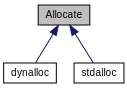
\includegraphics[width=200pt]{class_allocate__inherit__graph}
\end{center}
\end{figure}


Collaboration diagram for Allocate\+:
\nopagebreak
\begin{figure}[H]
\begin{center}
\leavevmode
\includegraphics[width=323pt]{class_allocate__coll__graph}
\end{center}
\end{figure}
\subsection*{Public Member Functions}
\begin{DoxyCompactItemize}
\item 
\hyperlink{class_allocate_ab2b82e7fab9d0fccb9702effec93917b}{Allocate} (\hyperlink{classraft_1_1map}{raft\+::map} \&map, volatile bool \&\hyperlink{class_allocate_a4d10076b88ab1297c89b8a05e117b510}{exit\+\_\+alloc})
\item 
virtual \hyperlink{class_allocate_a68cd61da26f3b82da094b6d3e5d556f5}{$\sim$\+Allocate} ()
\item 
virtual void \hyperlink{class_allocate_a44f9b51c382fec159233609e21b9d272}{run} ()=0
\item 
void \hyperlink{class_allocate_a3123c2c1d9584974ce19b47fe6ceea17}{wait\+Till\+Ready} ()
\end{DoxyCompactItemize}
\subsection*{Protected Member Functions}
\begin{DoxyCompactItemize}
\item 
void \hyperlink{class_allocate_a1d5c71b5cd6fc9671ed82d9c1d04965c}{initialize} (\hyperlink{struct_port_info}{Port\+Info} $\ast$const src, \hyperlink{struct_port_info}{Port\+Info} $\ast$const dst, \hyperlink{class_f_i_f_o}{F\+I\+FO} $\ast$const fifo)
\item 
\hypertarget{class_allocate_a901eb0fdb6cffd56019c9ab9f2b25f92}{}\label{class_allocate_a901eb0fdb6cffd56019c9ab9f2b25f92} 
virtual void {\bfseries allocate} (\hyperlink{struct_port_info}{Port\+Info} \&a, \hyperlink{struct_port_info}{Port\+Info} \&b, void $\ast$data)
\item 
void \hyperlink{class_allocate_a4cf36bb704e43f5736a0e736d9e1a81b}{set\+Ready} ()
\end{DoxyCompactItemize}
\subsection*{Protected Attributes}
\begin{DoxyCompactItemize}
\item 
kernelkeeper \& \hyperlink{class_allocate_a93e612d7ea7eb686fc88b5dee7a1407b}{source\+\_\+kernels}
\item 
\hypertarget{class_allocate_a91e8c7d69ab7b309ea45439aea54fb4f}{}\label{class_allocate_a91e8c7d69ab7b309ea45439aea54fb4f} 
kernelkeeper \& {\bfseries all\+\_\+kernels}
\item 
std\+::set$<$ \hyperlink{class_f_i_f_o}{F\+I\+FO} $\ast$$>$ \hyperlink{class_allocate_a037410210c0d10578f87de1ec68f47ba}{allocated\+\_\+fifo}
\item 
volatile bool \& \hyperlink{class_allocate_a4d10076b88ab1297c89b8a05e117b510}{exit\+\_\+alloc}
\end{DoxyCompactItemize}
\subsection*{Friends}
\begin{DoxyCompactItemize}
\item 
\hypertarget{class_allocate_a901ac6fe1c35f3c114cf9e83f75dde0c}{}\label{class_allocate_a901ac6fe1c35f3c114cf9e83f75dde0c} 
class {\bfseries basic\+\_\+parallel}
\end{DoxyCompactItemize}


\subsection{Detailed Description}


Definition at line 58 of file allocate.\+hpp.



\subsection{Constructor \& Destructor Documentation}
\hypertarget{class_allocate_ab2b82e7fab9d0fccb9702effec93917b}{}\label{class_allocate_ab2b82e7fab9d0fccb9702effec93917b} 
\index{Allocate@{Allocate}!Allocate@{Allocate}}
\index{Allocate@{Allocate}!Allocate@{Allocate}}
\subsubsection{\texorpdfstring{Allocate()}{Allocate()}}
{\footnotesize\ttfamily Allocate\+::\+Allocate (\begin{DoxyParamCaption}\item[{\hyperlink{classraft_1_1map}{raft\+::map} \&}]{map,  }\item[{volatile bool \&}]{exit\+\_\+alloc }\end{DoxyParamCaption})}

\hyperlink{class_allocate}{Allocate} -\/ base constructor, really doesn\textquotesingle{}t do too much save for setting the global variables all\+\_\+kernels and source\+\_\+kernels from the Map object. 
\begin{DoxyParams}{Parameters}
{\em map} & -\/ \hyperlink{classraft_1_1map}{raft\+::map}\& \\
\hline
{\em exit\+\_\+alloc} & -\/ bool used to terminate loop, for monitoring allocations, controlled by map object.\\
\hline
\end{DoxyParams}
allocate.\+cpp -\/ \begin{DoxyAuthor}{Author}
\+: Jonathan Beard 
\end{DoxyAuthor}
\begin{DoxyVersion}{Version}
\+: Tue Sep 16 20\+:20\+:06 2014
\end{DoxyVersion}
Copyright 2014 Jonathan Beard

Licensed under the Apache License, Version 2.\+0 (the \char`\"{}\+License\char`\"{}); you may not use this file except in compliance with the License. You may obtain a copy of the License at\+:

\href{http://www.apache.org/licenses/LICENSE-2.0}{\tt http\+://www.\+apache.\+org/licenses/\+L\+I\+C\+E\+N\+S\+E-\/2.\+0}

Unless required by applicable law or agreed to in writing, software distributed under the License is distributed on an \char`\"{}\+A\+S I\+S\char`\"{} B\+A\+S\+IS, W\+I\+T\+H\+O\+UT W\+A\+R\+R\+A\+N\+T\+I\+ES OR C\+O\+N\+D\+I\+T\+I\+O\+NS OF A\+NY K\+I\+ND, either express or implied. See the License for the specific language governing permissions and limitations under the License. 

Definition at line 30 of file src/allocate.\+cpp.


\begin{DoxyCode}
30                                                             :
31    \hyperlink{class_allocate_a93e612d7ea7eb686fc88b5dee7a1407b}{source\_kernels}( map.\hyperlink{class_map_base_a2541cb37a237e66fc88129f9f0b02f50}{source\_kernels} ),
32    all\_kernels(    map.\hyperlink{class_map_base_a2220cd630c5d00708f08d9bc70a48220}{all\_kernels} ),
33    \hyperlink{class_allocate_a4d10076b88ab1297c89b8a05e117b510}{exit\_alloc}( \hyperlink{class_allocate_a4d10076b88ab1297c89b8a05e117b510}{exit\_alloc} )
34 \{
35 \}
\end{DoxyCode}
\hypertarget{class_allocate_a68cd61da26f3b82da094b6d3e5d556f5}{}\label{class_allocate_a68cd61da26f3b82da094b6d3e5d556f5} 
\index{Allocate@{Allocate}!````~Allocate@{$\sim$\+Allocate}}
\index{````~Allocate@{$\sim$\+Allocate}!Allocate@{Allocate}}
\subsubsection{\texorpdfstring{$\sim$\+Allocate()}{~Allocate()}}
{\footnotesize\ttfamily Allocate\+::$\sim$\+Allocate (\begin{DoxyParamCaption}{ }\end{DoxyParamCaption})\hspace{0.3cm}{\ttfamily [virtual]}}

destructor 

Definition at line 37 of file src/allocate.\+cpp.



References allocated\+\_\+fifo.


\begin{DoxyCode}
38 \{
39    \textcolor{keywordflow}{for}( \hyperlink{class_f_i_f_o}{FIFO} *f : \hyperlink{class_allocate_a037410210c0d10578f87de1ec68f47ba}{allocated\_fifo} )
40    \{
41       \textcolor{keyword}{delete}( f );
42    \}
43 \}
\end{DoxyCode}


\subsection{Member Function Documentation}
\hypertarget{class_allocate_a1d5c71b5cd6fc9671ed82d9c1d04965c}{}\label{class_allocate_a1d5c71b5cd6fc9671ed82d9c1d04965c} 
\index{Allocate@{Allocate}!initialize@{initialize}}
\index{initialize@{initialize}!Allocate@{Allocate}}
\subsubsection{\texorpdfstring{initialize()}{initialize()}}
{\footnotesize\ttfamily void Allocate\+::initialize (\begin{DoxyParamCaption}\item[{\hyperlink{struct_port_info}{Port\+Info} $\ast$const}]{src,  }\item[{\hyperlink{struct_port_info}{Port\+Info} $\ast$const}]{dst,  }\item[{\hyperlink{class_f_i_f_o}{F\+I\+FO} $\ast$const}]{fifo }\end{DoxyParamCaption})\hspace{0.3cm}{\ttfamily [protected]}}

initialize -\/ internal method to be used within the run method takes care of the initialization using the already allocated \hyperlink{class_f_i_f_o}{F\+I\+FO} object passed as a param. This function will throw an exception if either port (src or dst) have already been allocated. 
\begin{DoxyParams}{Parameters}
{\em src} & -\/ Port\+Info$\ast$, nullptr if not to be set \\
\hline
{\em dst} & -\/ Port\+Info$\ast$, nullptr if not to be set \\
\hline
{\em fifo} & -\/ F\+I\+F\+O$\ast$ \\
\hline
\end{DoxyParams}

\begin{DoxyExceptions}{Exceptions}
{\em \hyperlink{class_port_double_initialize_exception}{Port\+Double\+Initialize\+Exception}} & -\/ if either port is already initialized. \\
\hline
\end{DoxyExceptions}
N\+O\+TE\+: this list simply speeds up the monitoring if we want it 

Definition at line 58 of file src/allocate.\+cpp.



References allocated\+\_\+fifo, Port\+Info\+::const\+\_\+map, Port\+Info\+::get\+F\+I\+F\+O(), F\+I\+F\+O\+::set\+\_\+dst\+\_\+kernel(), F\+I\+F\+O\+::set\+\_\+src\+\_\+kernel(), and Port\+Info\+::set\+F\+I\+F\+O().



Referenced by stdalloc\+::run().


\begin{DoxyCode}
61 \{
62    assert( fifo != \textcolor{keyword}{nullptr} );
63    assert( dst  != \textcolor{keyword}{nullptr} );
64    assert( src  != \textcolor{keyword}{nullptr} );
65    \textcolor{keywordflow}{if}( src->\hyperlink{struct_port_info_a483d162fbe356e07381c6c5cfccb4f48}{getFIFO}() != nullptr )
66    \{
67       \textcolor{keywordflow}{throw} \hyperlink{class_port_double_initialize_exception}{PortDoubleInitializeException}(
68          \textcolor{stringliteral}{"Source port \(\backslash\)""} + src->my\_name + \textcolor{stringliteral}{"\(\backslash\)" already initialized!"} );
69    \}
70    \textcolor{keywordflow}{if}( dst->\hyperlink{struct_port_info_a483d162fbe356e07381c6c5cfccb4f48}{getFIFO}() !=  nullptr )
71    \{
72       \textcolor{keywordflow}{throw} \hyperlink{class_port_double_initialize_exception}{PortDoubleInitializeException}(
73          \textcolor{stringliteral}{"Destination port \(\backslash\)""} + dst->my\_name +  \textcolor{stringliteral}{"\(\backslash\)" already initialized!"} );
74    \}
75    src->\hyperlink{struct_port_info_a43a57cd624dcc44ccd9dcaba1d07a000}{setFIFO}( fifo );
76    fifo->\hyperlink{class_f_i_f_o_aa9c1f679b4e2585047af2c09a2518209}{set\_src\_kernel}( src->my\_kernel );
77    dst->\hyperlink{struct_port_info_a43a57cd624dcc44ccd9dcaba1d07a000}{setFIFO}( fifo );
78    fifo->\hyperlink{class_f_i_f_o_a11422695c75c05ad2c60e662553f2667}{set\_dst\_kernel}( dst->my\_kernel );\textcolor{comment}{}
79 \textcolor{comment}{   /** NOTE: this list simply speeds up the monitoring if we want it **/}
80    \hyperlink{class_allocate_a037410210c0d10578f87de1ec68f47ba}{allocated\_fifo}.insert( fifo );
81 \}
\end{DoxyCode}
Here is the call graph for this function\+:
\nopagebreak
\begin{figure}[H]
\begin{center}
\leavevmode
\includegraphics[width=318pt]{class_allocate_a1d5c71b5cd6fc9671ed82d9c1d04965c_cgraph}
\end{center}
\end{figure}
\hypertarget{class_allocate_a44f9b51c382fec159233609e21b9d272}{}\label{class_allocate_a44f9b51c382fec159233609e21b9d272} 
\index{Allocate@{Allocate}!run@{run}}
\index{run@{run}!Allocate@{Allocate}}
\subsubsection{\texorpdfstring{run()}{run()}}
{\footnotesize\ttfamily virtual void Allocate\+::run (\begin{DoxyParamCaption}{ }\end{DoxyParamCaption})\hspace{0.3cm}{\ttfamily [pure virtual]}}

run -\/ implement this function to create a new allocator, will be run inside a thread so exits when done but if run-\/time monitoring is desired then this is the place to do it. 

Implemented in \hyperlink{classstdalloc_a60438b15948ce354b52b03ba6d975de0}{stdalloc}, and \hyperlink{classdynalloc_a2a52b86ec09bd6dd52e49062137b2e37}{dynalloc}.

\hypertarget{class_allocate_a4cf36bb704e43f5736a0e736d9e1a81b}{}\label{class_allocate_a4cf36bb704e43f5736a0e736d9e1a81b} 
\index{Allocate@{Allocate}!set\+Ready@{set\+Ready}}
\index{set\+Ready@{set\+Ready}!Allocate@{Allocate}}
\subsubsection{\texorpdfstring{set\+Ready()}{setReady()}}
{\footnotesize\ttfamily void Allocate\+::set\+Ready (\begin{DoxyParamCaption}{ }\end{DoxyParamCaption})\hspace{0.3cm}{\ttfamily [protected]}}

set\+Ready -\/ call within the implemented run function to signal that the initial allocations have been completed. 

Definition at line 52 of file src/allocate.\+cpp.



Referenced by dynalloc\+::run(), and stdalloc\+::run().


\begin{DoxyCode}
53 \{
54    ready = \textcolor{keyword}{true};
55 \}
\end{DoxyCode}
\hypertarget{class_allocate_a3123c2c1d9584974ce19b47fe6ceea17}{}\label{class_allocate_a3123c2c1d9584974ce19b47fe6ceea17} 
\index{Allocate@{Allocate}!wait\+Till\+Ready@{wait\+Till\+Ready}}
\index{wait\+Till\+Ready@{wait\+Till\+Ready}!Allocate@{Allocate}}
\subsubsection{\texorpdfstring{wait\+Till\+Ready()}{waitTillReady()}}
{\footnotesize\ttfamily void Allocate\+::wait\+Till\+Ready (\begin{DoxyParamCaption}{ }\end{DoxyParamCaption})}

wait\+Till\+Ready -\/ call after initializing the allocate thread, returns when the initial allocation is complete. 

Definition at line 46 of file src/allocate.\+cpp.


\begin{DoxyCode}
47 \{
48    \textcolor{keywordflow}{while}( ! ready );
49 \}
\end{DoxyCode}


\subsection{Member Data Documentation}
\hypertarget{class_allocate_a037410210c0d10578f87de1ec68f47ba}{}\label{class_allocate_a037410210c0d10578f87de1ec68f47ba} 
\index{Allocate@{Allocate}!allocated\+\_\+fifo@{allocated\+\_\+fifo}}
\index{allocated\+\_\+fifo@{allocated\+\_\+fifo}!Allocate@{Allocate}}
\subsubsection{\texorpdfstring{allocated\+\_\+fifo}{allocated\_fifo}}
{\footnotesize\ttfamily std\+::set$<$ \hyperlink{class_f_i_f_o}{F\+I\+FO}$\ast$ $>$ Allocate\+::allocated\+\_\+fifo\hspace{0.3cm}{\ttfamily [protected]}}

keeps a list of all currently allocated \hyperlink{class_f_i_f_o}{F\+I\+FO} objects, set from within the initialize function. 

Definition at line 124 of file allocate.\+hpp.



Referenced by initialize(), and $\sim$\+Allocate().

\hypertarget{class_allocate_a4d10076b88ab1297c89b8a05e117b510}{}\label{class_allocate_a4d10076b88ab1297c89b8a05e117b510} 
\index{Allocate@{Allocate}!exit\+\_\+alloc@{exit\+\_\+alloc}}
\index{exit\+\_\+alloc@{exit\+\_\+alloc}!Allocate@{Allocate}}
\subsubsection{\texorpdfstring{exit\+\_\+alloc}{exit\_alloc}}
{\footnotesize\ttfamily volatile bool\& Allocate\+::exit\+\_\+alloc\hspace{0.3cm}{\ttfamily [protected]}}

exit\+\_\+alloc -\/ bool whose value is set by the map object, controls when the loop within the alloc thread is exited. 

Definition at line 131 of file allocate.\+hpp.



Referenced by dynalloc\+::run().

\hypertarget{class_allocate_a93e612d7ea7eb686fc88b5dee7a1407b}{}\label{class_allocate_a93e612d7ea7eb686fc88b5dee7a1407b} 
\index{Allocate@{Allocate}!source\+\_\+kernels@{source\+\_\+kernels}}
\index{source\+\_\+kernels@{source\+\_\+kernels}!Allocate@{Allocate}}
\subsubsection{\texorpdfstring{source\+\_\+kernels}{source\_kernels}}
{\footnotesize\ttfamily kernelkeeper\& Allocate\+::source\+\_\+kernels\hspace{0.3cm}{\ttfamily [protected]}}

both convenience structs, hold exactly what the names say 

Definition at line 117 of file allocate.\+hpp.



Referenced by dynalloc\+::run(), and stdalloc\+::run().



The documentation for this class was generated from the following files\+:\begin{DoxyCompactItemize}
\item 
allocate.\+hpp\item 
src/allocate.\+cpp\end{DoxyCompactItemize}

\hypertarget{class_ambiguous_port_assignment_exception}{}\section{Ambiguous\+Port\+Assignment\+Exception Class Reference}
\label{class_ambiguous_port_assignment_exception}\index{Ambiguous\+Port\+Assignment\+Exception@{Ambiguous\+Port\+Assignment\+Exception}}
Inheritance diagram for Ambiguous\+Port\+Assignment\+Exception\+:\begin{figure}[H]
\begin{center}
\leavevmode
\includegraphics[height=3.000000cm]{class_ambiguous_port_assignment_exception}
\end{center}
\end{figure}
\subsection*{Public Member Functions}
\begin{DoxyCompactItemize}
\item 
\hypertarget{class_ambiguous_port_assignment_exception_a5c2daf243080521a90629fcc262dec61}{}{\bfseries Ambiguous\+Port\+Assignment\+Exception} (const std\+::string message)\label{class_ambiguous_port_assignment_exception_a5c2daf243080521a90629fcc262dec61}

\end{DoxyCompactItemize}


The documentation for this class was generated from the following files\+:\begin{DoxyCompactItemize}
\item 
portexception.\+hpp\item 
portexception.\+cpp\end{DoxyCompactItemize}

\hypertarget{classbasic__parallel}{}\section{basic\+\_\+parallel Class Reference}
\label{classbasic__parallel}\index{basic\+\_\+parallel@{basic\+\_\+parallel}}
\subsection*{Public Member Functions}
\begin{DoxyCompactItemize}
\item 
\hyperlink{classbasic__parallel_a6f8a4933fb29d6f4c60ebb3e934b192e}{basic\+\_\+parallel} (\hyperlink{class_map}{Map} \&map, \hyperlink{class_allocate}{Allocate} \&alloc, \hyperlink{class_schedule}{Schedule} \&sched, volatile bool \&exit\+\_\+para)
\item 
virtual void \hyperlink{classbasic__parallel_a85ea2560d40ad50482468e39d626a52b}{start} ()
\end{DoxyCompactItemize}
\subsection*{Protected Attributes}
\begin{DoxyCompactItemize}
\item 
kernelkeeper \& \hyperlink{classbasic__parallel_a969b8832b2f6eaea5e985d4582d9e4dc}{source\+\_\+kernels}
\item 
\hypertarget{classbasic__parallel_a028feb03732d5fef0e9d184ddc18ce7b}{}kernelkeeper \& {\bfseries all\+\_\+kernels}\label{classbasic__parallel_a028feb03732d5fef0e9d184ddc18ce7b}

\item 
\hypertarget{classbasic__parallel_aab09daae41a9d218568115be037a8357}{}\hyperlink{class_allocate}{Allocate} \& {\bfseries alloc}\label{classbasic__parallel_aab09daae41a9d218568115be037a8357}

\item 
\hypertarget{classbasic__parallel_a9124d0bfd5d75277ddd44fb59814435a}{}\hyperlink{class_schedule}{Schedule} \& {\bfseries sched}\label{classbasic__parallel_a9124d0bfd5d75277ddd44fb59814435a}

\item 
\hypertarget{classbasic__parallel_ac648d03dceed09e7834d656f561da33b}{}volatile bool \& {\bfseries exit\+\_\+para}\label{classbasic__parallel_ac648d03dceed09e7834d656f561da33b}

\end{DoxyCompactItemize}


\subsection{Constructor \& Destructor Documentation}
\hypertarget{classbasic__parallel_a6f8a4933fb29d6f4c60ebb3e934b192e}{}\index{basic\+\_\+parallel@{basic\+\_\+parallel}!basic\+\_\+parallel@{basic\+\_\+parallel}}
\index{basic\+\_\+parallel@{basic\+\_\+parallel}!basic\+\_\+parallel@{basic\+\_\+parallel}}
\subsubsection[{basic\+\_\+parallel(\+Map \&map, Allocate \&alloc, Schedule \&sched, volatile bool \&exit\+\_\+para)}]{\setlength{\rightskip}{0pt plus 5cm}basic\+\_\+parallel\+::basic\+\_\+parallel (
\begin{DoxyParamCaption}
\item[{{\bf Map} \&}]{map, }
\item[{{\bf Allocate} \&}]{alloc, }
\item[{{\bf Schedule} \&}]{sched, }
\item[{volatile bool \&}]{exit\+\_\+para}
\end{DoxyParamCaption}
)}\label{classbasic__parallel_a6f8a4933fb29d6f4c60ebb3e934b192e}
nothing to do here, move along 

\subsection{Member Function Documentation}
\hypertarget{classbasic__parallel_a85ea2560d40ad50482468e39d626a52b}{}\index{basic\+\_\+parallel@{basic\+\_\+parallel}!start@{start}}
\index{start@{start}!basic\+\_\+parallel@{basic\+\_\+parallel}}
\subsubsection[{start()}]{\setlength{\rightskip}{0pt plus 5cm}void basic\+\_\+parallel\+::start (
\begin{DoxyParamCaption}
{}
\end{DoxyParamCaption}
)\hspace{0.3cm}{\ttfamily [virtual]}}\label{classbasic__parallel_a85ea2560d40ad50482468e39d626a52b}
since we have to have a lock on the ports for both B\+F\+S and duplication, we\textquotesingle{}ll mark the kernels inside of B\+F\+S and duplicate outside of it.

start checking stats

input stats

apply criteria

F\+I\+X\+M\+E, logic below only works for single input, single output..intended to get it working

clone

attach ports

connecting a.\+y -\/$>$ b.\+x new\+\_\+other\+\_\+outprt == port y on a new\+\_\+port\+\_\+in == port x on b

connecting b.\+y -\/$>$ c.\+x newoutport == port y on b new\+\_\+other\+\_\+inport == port x on c

schedule new kernel 

\subsection{Member Data Documentation}
\hypertarget{classbasic__parallel_a969b8832b2f6eaea5e985d4582d9e4dc}{}\index{basic\+\_\+parallel@{basic\+\_\+parallel}!source\+\_\+kernels@{source\+\_\+kernels}}
\index{source\+\_\+kernels@{source\+\_\+kernels}!basic\+\_\+parallel@{basic\+\_\+parallel}}
\subsubsection[{source\+\_\+kernels}]{\setlength{\rightskip}{0pt plus 5cm}kernelkeeper\& basic\+\_\+parallel\+::source\+\_\+kernels\hspace{0.3cm}{\ttfamily [protected]}}\label{classbasic__parallel_a969b8832b2f6eaea5e985d4582d9e4dc}
both convenience structs, hold exactly what the names say 

The documentation for this class was generated from the following files\+:\begin{DoxyCompactItemize}
\item 
basicparallel.\+hpp\item 
basicparallel.\+cpp\end{DoxyCompactItemize}

\hypertarget{class_closed_port_access_exception}{}\section{Closed\+Port\+Access\+Exception Class Reference}
\label{class_closed_port_access_exception}\index{Closed\+Port\+Access\+Exception@{Closed\+Port\+Access\+Exception}}


Inheritance diagram for Closed\+Port\+Access\+Exception\+:
\nopagebreak
\begin{figure}[H]
\begin{center}
\leavevmode
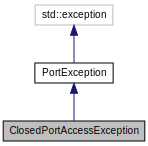
\includegraphics[width=222pt]{class_closed_port_access_exception__inherit__graph}
\end{center}
\end{figure}


Collaboration diagram for Closed\+Port\+Access\+Exception\+:
\nopagebreak
\begin{figure}[H]
\begin{center}
\leavevmode
\includegraphics[width=222pt]{class_closed_port_access_exception__coll__graph}
\end{center}
\end{figure}
\subsection*{Public Member Functions}
\begin{DoxyCompactItemize}
\item 
\hypertarget{class_closed_port_access_exception_aa66df922ca194ecd6431bd9cae0a4b24}{}\label{class_closed_port_access_exception_aa66df922ca194ecd6431bd9cae0a4b24} 
{\bfseries Closed\+Port\+Access\+Exception} (const std\+::string message)
\end{DoxyCompactItemize}


\subsection{Detailed Description}


Definition at line 63 of file portexception.\+hpp.



The documentation for this class was generated from the following files\+:\begin{DoxyCompactItemize}
\item 
portexception.\+hpp\item 
portexception.\+cpp\end{DoxyCompactItemize}

\hypertarget{classcommon}{}\section{common Class Reference}
\label{classcommon}\index{common@{common}}


{\ttfamily \#include $<$common.\+hpp$>$}

\subsection*{Static Public Member Functions}
\begin{DoxyCompactItemize}
\item 
static std\+::string \hyperlink{classcommon_a7ca2338596041e14a38de0f63d1c1e31}{\+\_\+\+\_\+print\+Class\+Name} (const std\+::string \&\&obj\+\_\+name)
\item 
\hypertarget{classcommon_aa84197a1f03508da476a68d11fe139d5}{}\label{classcommon_aa84197a1f03508da476a68d11fe139d5} 
static std\+::string {\bfseries print\+Class\+Name\+From\+Str} (const std\+::string \&\&str)
\item 
{\footnotesize template$<$class K $>$ }\\static std\+::string \hyperlink{classcommon_aec4b942352abd180c71fca2c0dbd70b7}{print\+Class\+Name} (K \&k)
\end{DoxyCompactItemize}


\subsection{Detailed Description}
\hyperlink{common_8hpp_source}{common.\+hpp} -\/ static helper functions of various types \begin{DoxyAuthor}{Author}
\+: Jonathan Beard 
\end{DoxyAuthor}
\begin{DoxyVersion}{Version}
\+: Sun May 10 19\+:10\+:06 2015
\end{DoxyVersion}
Copyright 2015 Jonathan Beard

Licensed under the Apache License, Version 2.\+0 (the \char`\"{}\+License\char`\"{}); you may not use this file except in compliance with the License. You may obtain a copy of the License at\+:

\href{http://www.apache.org/licenses/LICENSE-2.0}{\tt http\+://www.\+apache.\+org/licenses/\+L\+I\+C\+E\+N\+S\+E-\/2.\+0}

Unless required by applicable law or agreed to in writing, software distributed under the License is distributed on an \char`\"{}\+A\+S I\+S\char`\"{} B\+A\+S\+IS, W\+I\+T\+H\+O\+UT W\+A\+R\+R\+A\+N\+T\+I\+ES OR C\+O\+N\+D\+I\+T\+I\+O\+NS OF A\+NY K\+I\+ND, either express or implied. See the License for the specific language governing permissions and limitations under the License. 

Definition at line 28 of file common.\+hpp.



\subsection{Member Function Documentation}
\hypertarget{classcommon_a7ca2338596041e14a38de0f63d1c1e31}{}\label{classcommon_a7ca2338596041e14a38de0f63d1c1e31} 
\index{common@{common}!\+\_\+\+\_\+print\+Class\+Name@{\+\_\+\+\_\+print\+Class\+Name}}
\index{\+\_\+\+\_\+print\+Class\+Name@{\+\_\+\+\_\+print\+Class\+Name}!common@{common}}
\subsubsection{\texorpdfstring{\+\_\+\+\_\+print\+Class\+Name()}{\_\_printClassName()}}
{\footnotesize\ttfamily std\+::string common\+::\+\_\+\+\_\+print\+Class\+Name (\begin{DoxyParamCaption}\item[{const std\+::string \&\&}]{obj\+\_\+name }\end{DoxyParamCaption})\hspace{0.3cm}{\ttfamily [static]}}

\+\_\+\+\_\+print\+Class\+Name -\/ helper function for below function, basically see the more complete docs below for the delta, the string passed to this function should be the name of the class from either the typeinfo or typeid( xx ).name() call. user must delete this, make string then delete 

Definition at line 7 of file common.\+cpp.



Referenced by print\+Class\+Name().


\begin{DoxyCode}
8 \{\textcolor{comment}{}
9 \textcolor{comment}{   /** user must delete this, make string then delete **/}
10    \textcolor{keywordflow}{return}( boost::core::demangle( obj\_name.c\_str() ) );
11 \}
\end{DoxyCode}
\hypertarget{classcommon_aec4b942352abd180c71fca2c0dbd70b7}{}\label{classcommon_aec4b942352abd180c71fca2c0dbd70b7} 
\index{common@{common}!print\+Class\+Name@{print\+Class\+Name}}
\index{print\+Class\+Name@{print\+Class\+Name}!common@{common}}
\subsubsection{\texorpdfstring{print\+Class\+Name()}{printClassName()}}
{\footnotesize\ttfamily template$<$class K $>$ \\
static std\+::string common\+::print\+Class\+Name (\begin{DoxyParamCaption}\item[{K \&}]{k }\end{DoxyParamCaption})\hspace{0.3cm}{\ttfamily [inline]}, {\ttfamily [static]}}

pring\+Class\+Name -\/ takes in a class reference and prints the class name using cxx-\/demangle. I basically got tired of typing all the error checking code over and over so here\textquotesingle{}s a simplified interface for it. 
\begin{DoxyParams}{Parameters}
{\em k} & -\/ Class reference for which you want the class. \\
\hline
\end{DoxyParams}
\begin{DoxyReturn}{Returns}
std\+::string 
\end{DoxyReturn}


Definition at line 51 of file common.\+hpp.



References \+\_\+\+\_\+print\+Class\+Name().



Referenced by Graph\+Tools\+::\+B\+F\+S(), and Map\+Base\+::join().


\begin{DoxyCode}
52 \{
53    \textcolor{keywordflow}{return}( \hyperlink{classcommon_a7ca2338596041e14a38de0f63d1c1e31}{common::\_\_printClassName}( \textcolor{keyword}{typeid}( k ).name() ) );
54 \}
\end{DoxyCode}
Here is the call graph for this function\+:
\nopagebreak
\begin{figure}[H]
\begin{center}
\leavevmode
\includegraphics[width=350pt]{classcommon_aec4b942352abd180c71fca2c0dbd70b7_cgraph}
\end{center}
\end{figure}


The documentation for this class was generated from the following files\+:\begin{DoxyCompactItemize}
\item 
common.\+hpp\item 
common.\+cpp\end{DoxyCompactItemize}

\hypertarget{classdynalloc}{}\section{dynalloc Class Reference}
\label{classdynalloc}\index{dynalloc@{dynalloc}}


Inheritance diagram for dynalloc\+:
\nopagebreak
\begin{figure}[H]
\begin{center}
\leavevmode
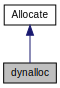
\includegraphics[width=133pt]{classdynalloc__inherit__graph}
\end{center}
\end{figure}


Collaboration diagram for dynalloc\+:
\nopagebreak
\begin{figure}[H]
\begin{center}
\leavevmode
\includegraphics[width=323pt]{classdynalloc__coll__graph}
\end{center}
\end{figure}
\subsection*{Public Member Functions}
\begin{DoxyCompactItemize}
\item 
\hyperlink{classdynalloc_ad5aa0343bab70d1f51e05953d890e8d2}{dynalloc} (\hyperlink{classraft_1_1map}{raft\+::map} \&map, volatile bool \&\hyperlink{class_allocate_a4d10076b88ab1297c89b8a05e117b510}{exit\+\_\+alloc})
\item 
virtual void \hyperlink{classdynalloc_a2a52b86ec09bd6dd52e49062137b2e37}{run} ()
\end{DoxyCompactItemize}
\subsection*{Additional Inherited Members}


\subsection{Detailed Description}


Definition at line 29 of file dynalloc.\+hpp.



\subsection{Constructor \& Destructor Documentation}
\hypertarget{classdynalloc_ad5aa0343bab70d1f51e05953d890e8d2}{}\label{classdynalloc_ad5aa0343bab70d1f51e05953d890e8d2} 
\index{dynalloc@{dynalloc}!dynalloc@{dynalloc}}
\index{dynalloc@{dynalloc}!dynalloc@{dynalloc}}
\subsubsection{\texorpdfstring{dynalloc()}{dynalloc()}}
{\footnotesize\ttfamily dynalloc\+::dynalloc (\begin{DoxyParamCaption}\item[{\hyperlink{classraft_1_1map}{raft\+::map} \&}]{map,  }\item[{volatile bool \&}]{exit\+\_\+alloc }\end{DoxyParamCaption})}

\hyperlink{dynalloc_8cpp_source}{dynalloc.\+cpp} -\/ \begin{DoxyAuthor}{Author}
\+: Jonathan Beard 
\end{DoxyAuthor}
\begin{DoxyVersion}{Version}
\+: Mon Oct 13 16\+:36\+:18 2014
\end{DoxyVersion}
Copyright 2014 Jonathan Beard

Licensed under the Apache License, Version 2.\+0 (the \char`\"{}\+License\char`\"{}); you may not use this file except in compliance with the License. You may obtain a copy of the License at\+:

\href{http://www.apache.org/licenses/LICENSE-2.0}{\tt http\+://www.\+apache.\+org/licenses/\+L\+I\+C\+E\+N\+S\+E-\/2.\+0}

Unless required by applicable law or agreed to in writing, software distributed under the License is distributed on an \char`\"{}\+A\+S I\+S\char`\"{} B\+A\+S\+IS, W\+I\+T\+H\+O\+UT W\+A\+R\+R\+A\+N\+T\+I\+ES OR C\+O\+N\+D\+I\+T\+I\+O\+NS OF A\+NY K\+I\+ND, either express or implied. See the License for the specific language governing permissions and limitations under the License. 

Definition at line 35 of file dynalloc.\+cpp.


\begin{DoxyCode}
36                                                 :
37                         \hyperlink{class_allocate_ab2b82e7fab9d0fccb9702effec93917b}{Allocate}( map, \hyperlink{class_allocate_a4d10076b88ab1297c89b8a05e117b510}{exit\_alloc} )
38 \{
39 \}
\end{DoxyCode}


\subsection{Member Function Documentation}
\hypertarget{classdynalloc_a2a52b86ec09bd6dd52e49062137b2e37}{}\label{classdynalloc_a2a52b86ec09bd6dd52e49062137b2e37} 
\index{dynalloc@{dynalloc}!run@{run}}
\index{run@{run}!dynalloc@{dynalloc}}
\subsubsection{\texorpdfstring{run()}{run()}}
{\footnotesize\ttfamily void dynalloc\+::run (\begin{DoxyParamCaption}{ }\end{DoxyParamCaption})\hspace{0.3cm}{\ttfamily [virtual]}}

run -\/ call to initiate schedule, in the current instantiation this is called by the scheduler. same alloc for all, inherit from base alloc

acquire source kernels

make this a fixed quantity right now, if size $>$ .75\% at montor interval three times or more then increase size.

T\+O\+DO, the values might wrap if no monitoring on

get initializer function

start monitor loop

monitor fifo\textquotesingle{}s 

Implements \hyperlink{class_allocate_a44f9b51c382fec159233609e21b9d272}{Allocate}.



Definition at line 65 of file dynalloc.\+cpp.



References Graph\+Tools\+::\+B\+F\+S(), Allocate\+::exit\+\_\+alloc, F\+I\+F\+O\+::get\+\_\+frac\+\_\+write\+\_\+blocked(), Port\+Info\+::get\+F\+I\+F\+O(), Allocate\+::set\+Ready(), and Allocate\+::source\+\_\+kernels.


\begin{DoxyCode}
66 \{
67    \textcolor{keyword}{auto} alloc\_func = [&]( \hyperlink{struct_port_info}{PortInfo} &a, \hyperlink{struct_port_info}{PortInfo} &b, \textcolor{keywordtype}{void} *data )
68    \{\textcolor{comment}{}
69 \textcolor{comment}{      /** same alloc for all, inherit from base alloc **/}
70       (\textcolor{keyword}{this})->allocate( a, b, data );
71    \};
72 \textcolor{comment}{}
73 \textcolor{comment}{   /** acquire source kernels **/}
74    \textcolor{keyword}{auto} &container( (\textcolor{keyword}{this})->\hyperlink{class_allocate_a93e612d7ea7eb686fc88b5dee7a1407b}{source\_kernels}.acquire() );
75    \hyperlink{class_graph_tools_ade51007699cbd681c1a37946609c46ee}{GraphTools::BFS}( container, alloc\_func );
76    (\textcolor{keyword}{this})->\hyperlink{class_allocate_a93e612d7ea7eb686fc88b5dee7a1407b}{source\_kernels}.release();
77    (\textcolor{keyword}{this})->\hyperlink{class_allocate_a4cf36bb704e43f5736a0e736d9e1a81b}{setReady}();
78    std::map< std::size\_t, int > size\_map;
79 \textcolor{comment}{}
80 \textcolor{comment}{   /**}
81 \textcolor{comment}{    * make this a fixed quantity right now, if size > .75% at}
82 \textcolor{comment}{    * montor interval three times or more then increase size.}
83 \textcolor{comment}{    */}
84 
85    \textcolor{keyword}{auto} mon\_func = [&]( \hyperlink{struct_port_info}{PortInfo} &a, \hyperlink{struct_port_info}{PortInfo} &b, \textcolor{keywordtype}{void} *data ) -> \textcolor{keywordtype}{void}
86    \{
87       (void) data;
88 
89       \textcolor{keyword}{const} \textcolor{keyword}{auto} hash\_val( dynalloc::hash( a, b ) );\textcolor{comment}{}
90 \textcolor{comment}{      /** TODO, the values might wrap if no monitoring on **/}
91       \textcolor{keyword}{const} \textcolor{keyword}{auto} realized\_ratio( a.\hyperlink{struct_port_info_a483d162fbe356e07381c6c5cfccb4f48}{getFIFO}()->\hyperlink{class_f_i_f_o_a4d44784c43a4026508e85982eb3174c7}{get\_frac\_write\_blocked}() );
92       \textcolor{keyword}{const} \textcolor{keyword}{auto} ratio( 0.8 );
93       \textcolor{keywordflow}{if}( realized\_ratio >= ratio )
94       \{
95          \textcolor{keyword}{const} \textcolor{keyword}{auto} curr\_count( size\_map[ hash\_val ]++ );
96          \textcolor{keywordflow}{if}( curr\_count  > 2 )
97          \{\textcolor{comment}{}
98 \textcolor{comment}{            /** get initializer function **/}
99             \textcolor{keyword}{auto} * \textcolor{keyword}{const} buff\_ptr( a.\hyperlink{struct_port_info_a483d162fbe356e07381c6c5cfccb4f48}{getFIFO}() );
100             \textcolor{keyword}{const} \textcolor{keyword}{auto} cap( buff\_ptr->capacity() );
101             buff\_ptr->resize( cap * 2, ALLOC\_ALIGN\_WIDTH, \hyperlink{class_allocate_a4d10076b88ab1297c89b8a05e117b510}{exit\_alloc} );
102             size\_map[ hash\_val ] = 0;
103          \}
104       \}
105       \textcolor{keywordflow}{return};
106    \};\textcolor{comment}{}
107 \textcolor{comment}{   /** start monitor loop **/}
108    \textcolor{keywordflow}{while}( ! \hyperlink{class_allocate_a4d10076b88ab1297c89b8a05e117b510}{exit\_alloc} )
109    \{\textcolor{comment}{}
110 \textcolor{comment}{      /** monitor fifo's **/}
111       std::chrono::microseconds dura( 3000 );
112       std::this\_thread::sleep\_for( dura );
113 
114       \textcolor{keyword}{auto} &container( (\textcolor{keyword}{this})->\hyperlink{class_allocate_a93e612d7ea7eb686fc88b5dee7a1407b}{source\_kernels}.acquire() );
115       \hyperlink{class_graph_tools_ade51007699cbd681c1a37946609c46ee}{GraphTools::BFS}( container, mon\_func );
116       (\textcolor{keyword}{this})->\hyperlink{class_allocate_a93e612d7ea7eb686fc88b5dee7a1407b}{source\_kernels}.release();
117 
118    \}
119    \textcolor{keywordflow}{return};
120 \}
\end{DoxyCode}
Here is the call graph for this function\+:
\nopagebreak
\begin{figure}[H]
\begin{center}
\leavevmode
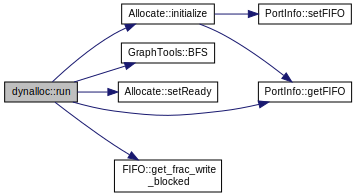
\includegraphics[width=296pt]{classdynalloc_a2a52b86ec09bd6dd52e49062137b2e37_cgraph}
\end{center}
\end{figure}


The documentation for this class was generated from the following files\+:\begin{DoxyCompactItemize}
\item 
dynalloc.\+hpp\item 
dynalloc.\+cpp\end{DoxyCompactItemize}

\hypertarget{class_graph_tools}{}\section{Graph\+Tools Class Reference}
\label{class_graph_tools}\index{Graph\+Tools@{Graph\+Tools}}
\subsection*{Static Public Member Functions}
\begin{DoxyCompactItemize}
\item 
static void \hyperlink{class_graph_tools_ade51007699cbd681c1a37946609c46ee}{B\+FS} (std\+::set$<$ \hyperlink{classraft_1_1kernel}{raft\+::kernel} $\ast$ $>$ \&source\+\_\+kernels, edge\+\_\+func func, void $\ast$data=nullptr, bool connected\+\_\+error=false)
\item 
static void \hyperlink{class_graph_tools_afc9c2852a351fe8b1a881b5d8b6c97f5}{B\+FS} (std\+::vector$<$ \hyperlink{classraft_1_1kernel}{raft\+::kernel} $\ast$ $>$ \&source\+\_\+kernels, edge\+\_\+func func, void $\ast$data=nullptr, bool connected\+\_\+error=false)
\item 
\hypertarget{class_graph_tools_a4223eca1b9bdb5b2b551f79b1faa155f}{}\label{class_graph_tools_a4223eca1b9bdb5b2b551f79b1faa155f} 
static void {\bfseries B\+FS} (std\+::set$<$ \hyperlink{classraft_1_1kernel}{raft\+::kernel} $\ast$ $>$ \&source\+\_\+kernels, vertex\+\_\+func func, void $\ast$data)
\end{DoxyCompactItemize}


\subsection{Detailed Description}


Definition at line 56 of file graphtools.\+hpp.



\subsection{Member Function Documentation}
\hypertarget{class_graph_tools_ade51007699cbd681c1a37946609c46ee}{}\label{class_graph_tools_ade51007699cbd681c1a37946609c46ee} 
\index{Graph\+Tools@{Graph\+Tools}!B\+FS@{B\+FS}}
\index{B\+FS@{B\+FS}!Graph\+Tools@{Graph\+Tools}}
\subsubsection{\texorpdfstring{B\+F\+S()}{BFS()}\hspace{0.1cm}{\footnotesize\ttfamily [1/2]}}
{\footnotesize\ttfamily void Graph\+Tools\+::\+B\+FS (\begin{DoxyParamCaption}\item[{std\+::set$<$ \hyperlink{classraft_1_1kernel}{raft\+::kernel} $\ast$ $>$ \&}]{source\+\_\+kernels,  }\item[{edge\+\_\+func}]{func,  }\item[{void $\ast$}]{data = {\ttfamily nullptr},  }\item[{bool}]{connected\+\_\+error = {\ttfamily false} }\end{DoxyParamCaption})\hspace{0.3cm}{\ttfamily [static]}}

B\+FS -\/ perform a breadth first search of the graph given by \textquotesingle{}source\+\_\+kernels\textquotesingle{}. The function \textquotesingle{}func\textquotesingle{} matches the typedef above and is called on each edge of the graph exactly once. For state between calls, the user can define a data struct and pass it via the void ptr data which is passed to the func. 
\begin{DoxyParams}{Parameters}
{\em source\+\_\+kernels} & -\/ set of source kernels. \\
\hline
{\em func} & -\/ edge\+\_\+func, funciton to be called \\
\hline
{\em data} & -\/ void$\ast$, data struct for persistent state \\
\hline
{\em connected\+\_\+error,throw} & an error if not connected\\
\hline
\end{DoxyParams}
\hyperlink{graphtools_8cpp_source}{graphtools.\+cpp} -\/ \begin{DoxyAuthor}{Author}
\+: Jonathan Beard 
\end{DoxyAuthor}
\begin{DoxyVersion}{Version}
\+: Sat Sep 20 13\+:15\+:09 2014
\end{DoxyVersion}
Copyright 2014 Jonathan Beard

Licensed under the Apache License, Version 2.\+0 (the \char`\"{}\+License\char`\"{}); you may not use this file except in compliance with the License. You may obtain a copy of the License at\+:

\href{http://www.apache.org/licenses/LICENSE-2.0}{\tt http\+://www.\+apache.\+org/licenses/\+L\+I\+C\+E\+N\+S\+E-\/2.\+0}

Unless required by applicable law or agreed to in writing, software distributed under the License is distributed on an \char`\"{}\+A\+S I\+S\char`\"{} B\+A\+S\+IS, W\+I\+T\+H\+O\+UT W\+A\+R\+R\+A\+N\+T\+I\+ES OR C\+O\+N\+D\+I\+T\+I\+O\+NS OF A\+NY K\+I\+ND, either express or implied. See the License for the specific language governing permissions and limitations under the License. 

Definition at line 38 of file graphtools.\+cpp.



Referenced by B\+F\+S(), raft\+::map\+::check\+Edges(), raft\+::map\+::enable\+Duplication(), dynalloc\+::run(), stdalloc\+::run(), and basic\+\_\+parallel\+::start().


\begin{DoxyCode}
42 \{
43    std::set< raft::kernel* > visited\_set;
44    std::queue< raft::kernel* >     queue;
45    std::for\_each( source\_kernels.begin(),
46                   source\_kernels.end(),
47                   [&]( \hyperlink{classraft_1_1kernel}{raft::kernel} *k )
48                   \{
49                      queue.push( k );
50                      visited\_set.insert( k );
51                   \} );
52    GraphTools::\_\_BFS( queue, visited\_set, func, data, connected\_error );
53 \}
\end{DoxyCode}
\hypertarget{class_graph_tools_afc9c2852a351fe8b1a881b5d8b6c97f5}{}\label{class_graph_tools_afc9c2852a351fe8b1a881b5d8b6c97f5} 
\index{Graph\+Tools@{Graph\+Tools}!B\+FS@{B\+FS}}
\index{B\+FS@{B\+FS}!Graph\+Tools@{Graph\+Tools}}
\subsubsection{\texorpdfstring{B\+F\+S()}{BFS()}\hspace{0.1cm}{\footnotesize\ttfamily [2/2]}}
{\footnotesize\ttfamily void Graph\+Tools\+::\+B\+FS (\begin{DoxyParamCaption}\item[{std\+::vector$<$ \hyperlink{classraft_1_1kernel}{raft\+::kernel} $\ast$ $>$ \&}]{source\+\_\+kernels,  }\item[{edge\+\_\+func}]{func,  }\item[{void $\ast$}]{data = {\ttfamily nullptr},  }\item[{bool}]{connected\+\_\+error = {\ttfamily false} }\end{DoxyParamCaption})\hspace{0.3cm}{\ttfamily [static]}}

B\+FS -\/ perform a breadth first search of the graph given by \textquotesingle{}source\+\_\+kernels\textquotesingle{}. The function \textquotesingle{}func\textquotesingle{} matches the typedef above and is called on each edge of the graph exactly once. For state between calls, the user can define a data struct and pass it via the void ptr data which is passed to the func. 
\begin{DoxyParams}{Parameters}
{\em source\+\_\+kernels} & -\/ set of source kernels. \\
\hline
{\em func} & -\/ edge\+\_\+func, funciton to be called \\
\hline
{\em data} & -\/ void$\ast$, data struct for persistent state \\
\hline
{\em connected\+\_\+error,throw} & an error if not connected \\
\hline
\end{DoxyParams}


Definition at line 56 of file graphtools.\+cpp.



References B\+F\+S(), Port\+::get\+Port\+Info\+For(), raft\+::kernel\+::input, Port\+::portmap, and common\+::print\+Class\+Name().


\begin{DoxyCode}
60 \{
61    std::set< raft::kernel* >       visited\_set;
62    std::queue< raft::kernel* >     queue;
63    std::for\_each( source\_kernels.begin(),
64                   source\_kernels.end(),
65                   [&]( \hyperlink{classraft_1_1kernel}{raft::kernel} *k )
66                   \{
67                      queue.push( k );
68                      visited\_set.insert( k );
69                   \} );
70    GraphTools::\_\_BFS( queue, visited\_set, func, data, connected\_error );
71 \}
\end{DoxyCode}
Here is the call graph for this function\+:
\nopagebreak
\begin{figure}[H]
\begin{center}
\leavevmode
\includegraphics[width=350pt]{class_graph_tools_afc9c2852a351fe8b1a881b5d8b6c97f5_cgraph}
\end{center}
\end{figure}


The documentation for this class was generated from the following files\+:\begin{DoxyCompactItemize}
\item 
graphtools.\+hpp\item 
graphtools.\+cpp\end{DoxyCompactItemize}

\hypertarget{classraft_1_1join}{}\section{raft\+:\+:join$<$ T, method $>$ Class Template Reference}
\label{classraft_1_1join}\index{raft\+::join$<$ T, method $>$@{raft\+::join$<$ T, method $>$}}


The documentation for this class was generated from the following file\+:\begin{DoxyCompactItemize}
\item 
port.\+hpp\end{DoxyCompactItemize}

\hypertarget{classraft_1_1kernel}{}\section{raft\+:\+:kernel Class Reference}
\label{classraft_1_1kernel}\index{raft\+::kernel@{raft\+::kernel}}


Inheritance diagram for raft\+:\+:kernel\+:
\nopagebreak
\begin{figure}[H]
\begin{center}
\leavevmode
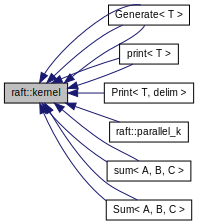
\includegraphics[width=264pt]{classraft_1_1kernel__inherit__graph}
\end{center}
\end{figure}


Collaboration diagram for raft\+:\+:kernel\+:
\nopagebreak
\begin{figure}[H]
\begin{center}
\leavevmode
\includegraphics[width=350pt]{classraft_1_1kernel__coll__graph}
\end{center}
\end{figure}
\subsection*{Public Member Functions}
\begin{DoxyCompactItemize}
\item 
\hyperlink{classraft_1_1kernel_a57aa6c7842f594d1522fb1c127fc4588}{kernel} ()
\item 
\hyperlink{classraft_1_1kernel_a8c275f04f04b99d77fc4639a053112c8}{kernel} (void $\ast$const ptr, const std\+::size\+\_\+t nbytes)
\item 
virtual raft\+::kstatus \hyperlink{classraft_1_1kernel_a05094286d7577360fb1b91c91fc05901}{run} ()=0
\item 
virtual \hyperlink{classraft_1_1kernel}{raft\+::kernel} $\ast$ \hyperlink{classraft_1_1kernel_a71bfffbbb3d40949e19be32e3d8f467f}{clone} ()
\item 
\hypertarget{classraft_1_1kernel_a2376ee5c5d413955db3f017fb707a6df}{}\label{classraft_1_1kernel_a2376ee5c5d413955db3f017fb707a6df} 
std\+::size\+\_\+t {\bfseries get\+\_\+id} ()
\item 
\hyperlink{classraft_1_1kernel}{raft\+::kernel} \& \hyperlink{classraft_1_1kernel_a186ea784c5b1ac8fd90f2112c1c62675}{operator\mbox{[}$\,$\mbox{]}} (const std\+::string \&\&portname)
\item 
\hypertarget{classraft_1_1kernel_aafd70e8e6ff6137db295e8dd0388b77d}{}\label{classraft_1_1kernel_aafd70e8e6ff6137db295e8dd0388b77d} 
core\+\_\+id\+\_\+t {\bfseries get\+Core\+Assignment} () noexcept
\end{DoxyCompactItemize}
\subsection*{Static Public Member Functions}
\begin{DoxyCompactItemize}
\item 
\hypertarget{classraft_1_1kernel_aebbcef35d4e08abbbe4167c2b75fab5f}{}\label{classraft_1_1kernel_aebbcef35d4e08abbbe4167c2b75fab5f} 
{\footnotesize template$<$class T , class ... Args$>$ }\\static \hyperlink{classraft_1_1kernel__wrapper}{kernel\+\_\+wrapper} {\bfseries make} (Args \&\&... params)
\end{DoxyCompactItemize}
\subsection*{Protected Member Functions}
\begin{DoxyCompactItemize}
\item 
\hypertarget{classraft_1_1kernel_ab206ff6ee1b729ab8875e181cbef227f}{}\label{classraft_1_1kernel_ab206ff6ee1b729ab8875e181cbef227f} 
virtual std\+::size\+\_\+t {\bfseries add\+Port} ()
\item 
virtual void \hyperlink{classraft_1_1kernel_abd7f3bf1f689840f7d61f472f520c258}{lock} ()
\item 
virtual void \hyperlink{classraft_1_1kernel_a7966dcabb0ed65ac52f6f78918256861}{unlock} ()
\item 
\hypertarget{classraft_1_1kernel_ad463ccfdb7d7e5360cba78bec277cbfe}{}\label{classraft_1_1kernel_ad463ccfdb7d7e5360cba78bec277cbfe} 
std\+::string {\bfseries get\+Enabled\+Port} ()
\item 
\hypertarget{classraft_1_1kernel_a0615a961de9038101c266e69fe2994ca}{}\label{classraft_1_1kernel_a0615a961de9038101c266e69fe2994ca} 
void {\bfseries retire} () noexcept
\item 
\hypertarget{classraft_1_1kernel_a41f090e0b3a4cf96471207155f6af80a}{}\label{classraft_1_1kernel_a41f090e0b3a4cf96471207155f6af80a} 
bool {\bfseries is\+Retired} () noexcept
\item 
\hypertarget{classraft_1_1kernel_a070219cf511c97848218a3431952395c}{}\label{classraft_1_1kernel_a070219cf511c97848218a3431952395c} 
void {\bfseries set\+Core} (const core\+\_\+id\+\_\+t id) noexcept
\end{DoxyCompactItemize}
\subsection*{Protected Attributes}
\begin{DoxyCompactItemize}
\item 
\hyperlink{class_port}{Port} \hyperlink{classraft_1_1kernel_a6edbe35a56409d402e719b3ac36d6554}{input} = \{ this \}
\item 
\hypertarget{classraft_1_1kernel_a1c65cc76ecaa8880ba527e5a146ca4ba}{}\label{classraft_1_1kernel_a1c65cc76ecaa8880ba527e5a146ca4ba} 
\hyperlink{class_port}{Port} {\bfseries output} = \{ this \}
\item 
\hypertarget{classraft_1_1kernel_afc8b7b8a99c538a5f741309730832fc4}{}\label{classraft_1_1kernel_afc8b7b8a99c538a5f741309730832fc4} 
bool {\bfseries internal\+\_\+alloc} = false
\item 
\hypertarget{classraft_1_1kernel_af754bdc01acf6eea572d0ddcd89b568f}{}\label{classraft_1_1kernel_af754bdc01acf6eea572d0ddcd89b568f} 
core\+\_\+id\+\_\+t {\bfseries core\+\_\+assign} = -\/1
\end{DoxyCompactItemize}
\subsection*{Static Protected Attributes}
\begin{DoxyCompactItemize}
\item 
static std\+::size\+\_\+t \hyperlink{classraft_1_1kernel_a98e05f7418c208e28b9112e92df7eccf}{kernel\+\_\+count}
\end{DoxyCompactItemize}
\subsection*{Friends}
\begin{DoxyCompactItemize}
\item 
class \hyperlink{classraft_1_1kernel_aeda338414e516b47761f994fb78056c6}{map}
\item 
class \hyperlink{classraft_1_1kernel_a1045638a7591b3c72cd145fc541d6478}{\+::\+Map\+Base}
\item 
\hypertarget{classraft_1_1kernel_a59b0d31ff28240338a2b6e682030ca3c}{}\label{classraft_1_1kernel_a59b0d31ff28240338a2b6e682030ca3c} 
class {\bfseries \+::\+Schedule}
\item 
\hypertarget{classraft_1_1kernel_a24755791643232aebfeedaa4ff0ecf03}{}\label{classraft_1_1kernel_a24755791643232aebfeedaa4ff0ecf03} 
class {\bfseries \+::\+Graph\+Tools}
\item 
\hypertarget{classraft_1_1kernel_aa3a6c191bed2aef9502f837b67e786b2}{}\label{classraft_1_1kernel_aa3a6c191bed2aef9502f837b67e786b2} 
class {\bfseries \+::kernel\+\_\+container}
\item 
\hypertarget{classraft_1_1kernel_ae75d52e84ecfc11bcaa43dd9fe149a2f}{}\label{classraft_1_1kernel_ae75d52e84ecfc11bcaa43dd9fe149a2f} 
class {\bfseries \+::basic\+\_\+parallel}
\item 
\hypertarget{classraft_1_1kernel_ae07b02dff85bd74c2d4d69d55bafe0a2}{}\label{classraft_1_1kernel_ae07b02dff85bd74c2d4d69d55bafe0a2} 
class {\bfseries \+::kpair}
\item 
\hypertarget{classraft_1_1kernel_a6b0f0238fe633a6ff44089d4667d3a7a}{}\label{classraft_1_1kernel_a6b0f0238fe633a6ff44089d4667d3a7a} 
class {\bfseries \+::interface\+\_\+partition}
\item 
\hypertarget{classraft_1_1kernel_a24b9e107a2ae5dbaf9831c0acc54df32}{}\label{classraft_1_1kernel_a24b9e107a2ae5dbaf9831c0acc54df32} 
class {\bfseries \+::pool\+\_\+schedule}
\end{DoxyCompactItemize}


\subsection{Detailed Description}


Definition at line 64 of file kernel.\+hpp.



\subsection{Constructor \& Destructor Documentation}
\hypertarget{classraft_1_1kernel_a57aa6c7842f594d1522fb1c127fc4588}{}\label{classraft_1_1kernel_a57aa6c7842f594d1522fb1c127fc4588} 
\index{raft\+::kernel@{raft\+::kernel}!kernel@{kernel}}
\index{kernel@{kernel}!raft\+::kernel@{raft\+::kernel}}
\subsubsection{\texorpdfstring{kernel()}{kernel()}\hspace{0.1cm}{\footnotesize\ttfamily [1/2]}}
{\footnotesize\ttfamily kernel\+::kernel (\begin{DoxyParamCaption}{ }\end{DoxyParamCaption})}

default constructor

default 

Definition at line 10 of file kernel.\+cpp.



References kernel\+\_\+count.


\begin{DoxyCode}
10                : kernel\_id( \hyperlink{classraft_1_1kernel_a98e05f7418c208e28b9112e92df7eccf}{kernel::kernel\_count} )
11 \{
12    \hyperlink{classraft_1_1kernel_a98e05f7418c208e28b9112e92df7eccf}{kernel::kernel\_count}++;
13 \}
\end{DoxyCode}
\hypertarget{classraft_1_1kernel_a8c275f04f04b99d77fc4639a053112c8}{}\label{classraft_1_1kernel_a8c275f04f04b99d77fc4639a053112c8} 
\index{raft\+::kernel@{raft\+::kernel}!kernel@{kernel}}
\index{kernel@{kernel}!raft\+::kernel@{raft\+::kernel}}
\subsubsection{\texorpdfstring{kernel()}{kernel()}\hspace{0.1cm}{\footnotesize\ttfamily [2/2]}}
{\footnotesize\ttfamily kernel\+::kernel (\begin{DoxyParamCaption}\item[{void $\ast$const}]{ptr,  }\item[{const std\+::size\+\_\+t}]{nbytes }\end{DoxyParamCaption})}

in-\/place allocation

existing memory 

Definition at line 16 of file kernel.\+cpp.


\begin{DoxyCode}
17                                          :
18    \hyperlink{classraft_1_1kernel_a6edbe35a56409d402e719b3ac36d6554}{input}(  \textcolor{keyword}{this}, ptr, nbytes ),
19    output( \textcolor{keyword}{this}, ptr, nbytes ),
20    kernel\_id( \hyperlink{classraft_1_1kernel_a98e05f7418c208e28b9112e92df7eccf}{kernel::kernel\_count} )
21 \{
22 \}
\end{DoxyCode}


\subsection{Member Function Documentation}
\hypertarget{classraft_1_1kernel_a71bfffbbb3d40949e19be32e3d8f467f}{}\label{classraft_1_1kernel_a71bfffbbb3d40949e19be32e3d8f467f} 
\index{raft\+::kernel@{raft\+::kernel}!clone@{clone}}
\index{clone@{clone}!raft\+::kernel@{raft\+::kernel}}
\subsubsection{\texorpdfstring{clone()}{clone()}}
{\footnotesize\ttfamily virtual \hyperlink{classraft_1_1kernel}{raft\+::kernel}$\ast$ raft\+::kernel\+::clone (\begin{DoxyParamCaption}{ }\end{DoxyParamCaption})\hspace{0.3cm}{\ttfamily [inline]}, {\ttfamily [virtual]}}

clone -\/ used for parallelization of kernels, if necessary sub-\/kernels should include an appropriate copy constructor so all class member variables can be set. 
\begin{DoxyParams}{Parameters}
{\em other,T\&} & -\/ reference to object to be cloned \\
\hline
\end{DoxyParams}
\begin{DoxyReturn}{Returns}
kernel$\ast$ -\/ takes base type, however is same as allocated by copy constructor for T. 
\end{DoxyReturn}
won\textquotesingle{}t be reached 

Definition at line 105 of file kernel.\+hpp.



References lock(), operator\mbox{[}$\,$\mbox{]}(), and unlock().



Referenced by raft\+::map\+::operator+=(), and basic\+\_\+parallel\+::start().


\begin{DoxyCode}
106    \{
107       \textcolor{keywordflow}{throw} \hyperlink{class_clone_not_implemented_exception}{CloneNotImplementedException}( \textcolor{stringliteral}{"Sub-class has failed to implement
       clone function, please use the CLONE() macro to add functionality"} );\textcolor{comment}{}
108 \textcolor{comment}{      /** won't be reached **/}
109       \textcolor{keywordflow}{return}( \textcolor{keyword}{nullptr} );
110    \}
\end{DoxyCode}
Here is the call graph for this function\+:
\nopagebreak
\begin{figure}[H]
\begin{center}
\leavevmode
\includegraphics[width=320pt]{classraft_1_1kernel_a71bfffbbb3d40949e19be32e3d8f467f_cgraph}
\end{center}
\end{figure}
\hypertarget{classraft_1_1kernel_abd7f3bf1f689840f7d61f472f520c258}{}\label{classraft_1_1kernel_abd7f3bf1f689840f7d61f472f520c258} 
\index{raft\+::kernel@{raft\+::kernel}!lock@{lock}}
\index{lock@{lock}!raft\+::kernel@{raft\+::kernel}}
\subsubsection{\texorpdfstring{lock()}{lock()}}
{\footnotesize\ttfamily void kernel\+::lock (\begin{DoxyParamCaption}{ }\end{DoxyParamCaption})\hspace{0.3cm}{\ttfamily [protected]}, {\ttfamily [virtual]}}

does nothing, just need a base impl 

Definition at line 54 of file kernel.\+cpp.



Referenced by clone().


\begin{DoxyCode}
55 \{\textcolor{comment}{}
56 \textcolor{comment}{   /** does nothing, just need a base impl **/}
57    \textcolor{keywordflow}{return};
58 \}
\end{DoxyCode}
\hypertarget{classraft_1_1kernel_a186ea784c5b1ac8fd90f2112c1c62675}{}\label{classraft_1_1kernel_a186ea784c5b1ac8fd90f2112c1c62675} 
\index{raft\+::kernel@{raft\+::kernel}!operator\mbox{[}\mbox{]}@{operator[]}}
\index{operator\mbox{[}\mbox{]}@{operator[]}!raft\+::kernel@{raft\+::kernel}}
\subsubsection{\texorpdfstring{operator[]()}{operator[]()}}
{\footnotesize\ttfamily \hyperlink{classraft_1_1kernel}{raft\+::kernel} \& kernel\+::operator\mbox{[}$\,$\mbox{]} (\begin{DoxyParamCaption}\item[{const std\+::string \&\&}]{portname }\end{DoxyParamCaption})}

operator\mbox{[}\mbox{]} -\/ returns the current kernel with the specified port name enabled for linking. 
\begin{DoxyParams}{Parameters}
{\em portname} & -\/ const std\+::string\&\& \\
\hline
\end{DoxyParams}
\begin{DoxyReturn}{Returns}
\hyperlink{classraft_1_1kernel}{raft\+::kernel}\&\& 
\end{DoxyReturn}


Definition at line 32 of file kernel.\+cpp.



Referenced by clone().


\begin{DoxyCode}
33 \{
34    \textcolor{keywordflow}{if}( enabled\_port.size() < 2 )
35    \{
36         enabled\_port.push( portname );
37    \}
38    \textcolor{keywordflow}{else}
39    \{
40         \textcolor{keywordflow}{throw} \hyperlink{class_ambiguous_port_assignment_exception}{AmbiguousPortAssignmentException}(
41             \textcolor{stringliteral}{"too many ports added with: "} + portname
42         );
43    \}
44    \textcolor{keywordflow}{return}( (*\textcolor{keyword}{this}) );
45 \}
\end{DoxyCode}
\hypertarget{classraft_1_1kernel_a05094286d7577360fb1b91c91fc05901}{}\label{classraft_1_1kernel_a05094286d7577360fb1b91c91fc05901} 
\index{raft\+::kernel@{raft\+::kernel}!run@{run}}
\index{run@{run}!raft\+::kernel@{raft\+::kernel}}
\subsubsection{\texorpdfstring{run()}{run()}}
{\footnotesize\ttfamily virtual raft\+::kstatus raft\+::kernel\+::run (\begin{DoxyParamCaption}{ }\end{DoxyParamCaption})\hspace{0.3cm}{\ttfamily [pure virtual]}}

run -\/ function to be extended for the actual execution. Code can be executed outside of the run function, i.\+e., with any function call, however the scheduler will only call the run function so it must initiate any follow-\/on behavior desired by the user. 

Implemented in \hyperlink{classlast_a7a1da1c30f571a8e8ccb515ca2cb2f02}{last}, \hyperlink{classlast_a7a1da1c30f571a8e8ccb515ca2cb2f02}{last}, \hyperlink{classlast_a7a1da1c30f571a8e8ccb515ca2cb2f02}{last}, \hyperlink{classlast_a7a1da1c30f571a8e8ccb515ca2cb2f02}{last}, \hyperlink{classmiddle_a9aa7415c102af751be9c7af4771b6f16}{middle}, \hyperlink{classlast_a7a1da1c30f571a8e8ccb515ca2cb2f02}{last}, \hyperlink{classmiddle_a9aa7415c102af751be9c7af4771b6f16}{middle}, \hyperlink{classmiddle_a9aa7415c102af751be9c7af4771b6f16}{middle}, \hyperlink{classmiddle_a9aa7415c102af751be9c7af4771b6f16}{middle}, \hyperlink{classlast_a7a1da1c30f571a8e8ccb515ca2cb2f02}{last}, \hyperlink{classstart_a4c076d756e2846f51e54452853a9ed6d}{start}, \hyperlink{classstart_a4c076d756e2846f51e54452853a9ed6d}{start}, \hyperlink{classstart_a4c076d756e2846f51e54452853a9ed6d}{start}, \hyperlink{classstart_a4c076d756e2846f51e54452853a9ed6d}{start}, \hyperlink{classstart_a4c076d756e2846f51e54452853a9ed6d}{start}, \hyperlink{classsub_a0a0c7461433ee8b5f4b24305282bf69a}{sub$<$ T $>$}, \hyperlink{classdisplay_a8652ca329ee5d1650e183b17f7299b51}{display$<$ T $>$}, \hyperlink{classsub_a0a0c7461433ee8b5f4b24305282bf69a}{sub$<$ T $>$}, \hyperlink{classsub_a0a0c7461433ee8b5f4b24305282bf69a}{sub$<$ T $>$}, \hyperlink{classsub_a0a0c7461433ee8b5f4b24305282bf69a}{sub$<$ T $>$}, \hyperlink{classsub_a0a0c7461433ee8b5f4b24305282bf69a}{sub$<$ T $>$}, \hyperlink{classsub_a0a0c7461433ee8b5f4b24305282bf69a}{sub$<$ T $>$}, \hyperlink{classsub_a0a0c7461433ee8b5f4b24305282bf69a}{sub$<$ T $>$}, \hyperlink{classsub_a0a0c7461433ee8b5f4b24305282bf69a}{sub$<$ T $>$}, \hyperlink{classsub_a0a0c7461433ee8b5f4b24305282bf69a}{sub$<$ T $>$}, \hyperlink{classsub_a0a0c7461433ee8b5f4b24305282bf69a}{sub$<$ T $>$}, \hyperlink{classsub_a0a0c7461433ee8b5f4b24305282bf69a}{sub$<$ T $>$}, \hyperlink{classsub_a0a0c7461433ee8b5f4b24305282bf69a}{sub$<$ T $>$}, \hyperlink{classstart_a4c076d756e2846f51e54452853a9ed6d}{start}, \hyperlink{classsource_ad144988607882cbe591a4c71642cb77a}{source$<$ T $>$}, \hyperlink{class_sum_ab915892675d11a8f3f0de2e7f96b0d28}{Sum$<$ A, B, C $>$}, \hyperlink{class_sum_ab915892675d11a8f3f0de2e7f96b0d28}{Sum$<$ A, B, C $>$}, \hyperlink{class_sum_ab915892675d11a8f3f0de2e7f96b0d28}{Sum$<$ A, B, C $>$}, \hyperlink{classprint_aa547f61c584b4044e4a0dfc2410e5adc}{print$<$ T $>$}, \hyperlink{class_generate_aa8253370207e1457b9b79e62253c2925}{Generate$<$ T $>$}, and \hyperlink{classsum_a2d0fac9129b826678d00520621937b15}{sum$<$ T $>$}.



Referenced by Schedule\+::kernel\+Run().

\hypertarget{classraft_1_1kernel_a7966dcabb0ed65ac52f6f78918256861}{}\label{classraft_1_1kernel_a7966dcabb0ed65ac52f6f78918256861} 
\index{raft\+::kernel@{raft\+::kernel}!unlock@{unlock}}
\index{unlock@{unlock}!raft\+::kernel@{raft\+::kernel}}
\subsubsection{\texorpdfstring{unlock()}{unlock()}}
{\footnotesize\ttfamily void kernel\+::unlock (\begin{DoxyParamCaption}{ }\end{DoxyParamCaption})\hspace{0.3cm}{\ttfamily [protected]}, {\ttfamily [virtual]}}

does nothing, just need a base impl 

Definition at line 61 of file kernel.\+cpp.



Referenced by clone().


\begin{DoxyCode}
62 \{\textcolor{comment}{}
63 \textcolor{comment}{   /** does nothing, just need a base impl **/}
64    \textcolor{keywordflow}{return};
65 \}
\end{DoxyCode}


\subsection{Friends And Related Function Documentation}
\hypertarget{classraft_1_1kernel_a1045638a7591b3c72cd145fc541d6478}{}\label{classraft_1_1kernel_a1045638a7591b3c72cd145fc541d6478} 
\index{raft\+::kernel@{raft\+::kernel}!\+::\+Map\+Base@{\+::\+Map\+Base}}
\index{\+::\+Map\+Base@{\+::\+Map\+Base}!raft\+::kernel@{raft\+::kernel}}
\subsubsection{\texorpdfstring{\+::\+Map\+Base}{::MapBase}}
{\footnotesize\ttfamily friend class \+::\hyperlink{class_map_base}{Map\+Base}\hspace{0.3cm}{\ttfamily [friend]}}

in global namespace 

Definition at line 149 of file kernel.\+hpp.

\hypertarget{classraft_1_1kernel_aeda338414e516b47761f994fb78056c6}{}\label{classraft_1_1kernel_aeda338414e516b47761f994fb78056c6} 
\index{raft\+::kernel@{raft\+::kernel}!map@{map}}
\index{map@{map}!raft\+::kernel@{raft\+::kernel}}
\subsubsection{\texorpdfstring{map}{map}}
{\footnotesize\ttfamily friend class \hyperlink{classraft_1_1map}{map}\hspace{0.3cm}{\ttfamily [friend]}}

in namespace raft 

Definition at line 147 of file kernel.\+hpp.



\subsection{Member Data Documentation}
\hypertarget{classraft_1_1kernel_a6edbe35a56409d402e719b3ac36d6554}{}\label{classraft_1_1kernel_a6edbe35a56409d402e719b3ac36d6554} 
\index{raft\+::kernel@{raft\+::kernel}!input@{input}}
\index{input@{input}!raft\+::kernel@{raft\+::kernel}}
\subsubsection{\texorpdfstring{input}{input}}
{\footnotesize\ttfamily \hyperlink{class_port}{Port} raft\+::kernel\+::input = \{ this \}\hspace{0.3cm}{\ttfamily [protected]}}

P\+O\+R\+TS -\/ input and output, use these to interact with the outside world. 

Definition at line 140 of file kernel.\+hpp.



Referenced by Graph\+Tools\+::\+B\+F\+S(), Schedule\+::check\+System\+Signal(), raft\+::map\+::enable\+Duplication(), Map\+Base\+::join(), Schedule\+::kernel\+Has\+Input\+Data(), Schedule\+::kernel\+Has\+No\+Input\+Ports(), kpair\+::kpair(), Map\+Base\+::link(), raft\+::map\+::operator+=(), sum$<$ T $>$\+::run(), print$<$ T $>$\+::run(), Sum$<$ A, B, C $>$\+::run(), start\+::run(), sub$<$ T $>$\+::run(), display$<$ T $>$\+::run(), last\+::run(), Schedule\+::schedule\+Kernel(), Schedule\+::set\+Ptr\+Sets(), and basic\+\_\+parallel\+::start().

\hypertarget{classraft_1_1kernel_a98e05f7418c208e28b9112e92df7eccf}{}\label{classraft_1_1kernel_a98e05f7418c208e28b9112e92df7eccf} 
\index{raft\+::kernel@{raft\+::kernel}!kernel\+\_\+count@{kernel\+\_\+count}}
\index{kernel\+\_\+count@{kernel\+\_\+count}!raft\+::kernel@{raft\+::kernel}}
\subsubsection{\texorpdfstring{kernel\+\_\+count}{kernel\_count}}
{\footnotesize\ttfamily std\+::size\+\_\+t kernel\+::kernel\+\_\+count\hspace{0.3cm}{\ttfamily [static]}, {\ttfamily [protected]}}

N\+O\+TE\+: doesn\textquotesingle{}t need to be atomic since only one thread will have responsibility to to create new compute kernels. 

Definition at line 163 of file kernel.\+hpp.



Referenced by kernel().



The documentation for this class was generated from the following files\+:\begin{DoxyCompactItemize}
\item 
kernel.\+hpp\item 
kernel.\+cpp\end{DoxyCompactItemize}

\hypertarget{classkernel__container}{}\section{kernel\+\_\+container Class Reference}
\label{classkernel__container}\index{kernel\+\_\+container@{kernel\+\_\+container}}
\subsection*{Public Types}
\begin{DoxyCompactItemize}
\item 
\hypertarget{classkernel__container_aaa8403088c93fca461e37158069d91b5}{}\label{classkernel__container_aaa8403088c93fca461e37158069d91b5} 
using {\bfseries buffer} = Ring\+Buffer$<$ \hyperlink{structsched__cmd__t}{sched\+\_\+cmd\+\_\+t}, Type\+::\+Ring\+Buffer\+Type\+::\+Heap, false $>$
\end{DoxyCompactItemize}
\subsection*{Public Member Functions}
\begin{DoxyCompactItemize}
\item 
\hyperlink{classkernel__container_a273d59eff9b9e269f1f9b231abc37b83}{kernel\+\_\+container} ()
\item 
\hyperlink{classkernel__container_a6d97cddd3d2f015166485afad9c71ff5}{kernel\+\_\+container} (const std\+::size\+\_\+t N)
\item 
\hyperlink{classkernel__container_acec164e3f4c6f37f4791c90c24514b34}{$\sim$kernel\+\_\+container} ()
\item 
buffer \& \hyperlink{classkernel__container_abcbec3854917b37bd6421b6b8ed2c2c0}{get\+Input\+Queue} ()
\item 
buffer \& \hyperlink{classkernel__container_a64384e258fee9b664d164eb50baf33df}{get\+Output\+Queue} ()
\item 
std\+::size\+\_\+t \hyperlink{classkernel__container_a358a15b772f1b7dfa57bd733fc78fcaa}{size} ()
\end{DoxyCompactItemize}
\subsection*{Static Public Member Functions}
\begin{DoxyCompactItemize}
\item 
static void \hyperlink{classkernel__container_a89f9b11119d9ab0e8c64215bf50856f0}{container\+\_\+run} (\hyperlink{classkernel__container}{kernel\+\_\+container} \&container)
\end{DoxyCompactItemize}


\subsection{Detailed Description}


Definition at line 36 of file kernelcontainer.\+hpp.



\subsection{Constructor \& Destructor Documentation}
\hypertarget{classkernel__container_a273d59eff9b9e269f1f9b231abc37b83}{}\label{classkernel__container_a273d59eff9b9e269f1f9b231abc37b83} 
\index{kernel\+\_\+container@{kernel\+\_\+container}!kernel\+\_\+container@{kernel\+\_\+container}}
\index{kernel\+\_\+container@{kernel\+\_\+container}!kernel\+\_\+container@{kernel\+\_\+container}}
\subsubsection{\texorpdfstring{kernel\+\_\+container()}{kernel\_container()}\hspace{0.1cm}{\footnotesize\ttfamily [1/2]}}
{\footnotesize\ttfamily kernel\+\_\+container\+::kernel\+\_\+container (\begin{DoxyParamCaption}{ }\end{DoxyParamCaption})}

\hyperlink{classkernel__container}{kernel\+\_\+container} -\/ default constructor, initializes all above pointers.

\hyperlink{kernelcontainer_8cpp_source}{kernelcontainer.\+cpp} -\/ \begin{DoxyAuthor}{Author}
\+: Jonathan Beard 
\end{DoxyAuthor}
\begin{DoxyVersion}{Version}
\+: Sun Mar 22 09\+:13\+:32 2015
\end{DoxyVersion}
Copyright 2015 Jonathan Beard

Licensed under the Apache License, Version 2.\+0 (the \char`\"{}\+License\char`\"{}); you may not use this file except in compliance with the License. You may obtain a copy of the License at\+:

\href{http://www.apache.org/licenses/LICENSE-2.0}{\tt http\+://www.\+apache.\+org/licenses/\+L\+I\+C\+E\+N\+S\+E-\/2.\+0}

Unless required by applicable law or agreed to in writing, software distributed under the License is distributed on an \char`\"{}\+A\+S I\+S\char`\"{} B\+A\+S\+IS, W\+I\+T\+H\+O\+UT W\+A\+R\+R\+A\+N\+T\+I\+ES OR C\+O\+N\+D\+I\+T\+I\+O\+NS OF A\+NY K\+I\+ND, either express or implied. See the License for the specific language governing permissions and limitations under the License. 

Definition at line 27 of file kernelcontainer.\+cpp.


\begin{DoxyCode}
28 \{
29    input\_buff  = \textcolor{keyword}{new} buffer( 100 );
30    output\_buff = \textcolor{keyword}{new} buffer( 100 );
31 \}
\end{DoxyCode}
\hypertarget{classkernel__container_a6d97cddd3d2f015166485afad9c71ff5}{}\label{classkernel__container_a6d97cddd3d2f015166485afad9c71ff5} 
\index{kernel\+\_\+container@{kernel\+\_\+container}!kernel\+\_\+container@{kernel\+\_\+container}}
\index{kernel\+\_\+container@{kernel\+\_\+container}!kernel\+\_\+container@{kernel\+\_\+container}}
\subsubsection{\texorpdfstring{kernel\+\_\+container()}{kernel\_container()}\hspace{0.1cm}{\footnotesize\ttfamily [2/2]}}
{\footnotesize\ttfamily kernel\+\_\+container\+::kernel\+\_\+container (\begin{DoxyParamCaption}\item[{const std\+::size\+\_\+t}]{N }\end{DoxyParamCaption})}

\hyperlink{classkernel__container}{kernel\+\_\+container} -\/ constructor, initializes all above pointers. 
\begin{DoxyParams}{Parameters}
{\em N} & -\/ const std\+::size\+\_\+t, default size of buffer \\
\hline
\end{DoxyParams}


Definition at line 33 of file kernelcontainer.\+cpp.


\begin{DoxyCode}
34 \{
35    input\_buff  = \textcolor{keyword}{new} buffer( N );
36    output\_buff = \textcolor{keyword}{new} buffer( N );
37 \}
\end{DoxyCode}
\hypertarget{classkernel__container_acec164e3f4c6f37f4791c90c24514b34}{}\label{classkernel__container_acec164e3f4c6f37f4791c90c24514b34} 
\index{kernel\+\_\+container@{kernel\+\_\+container}!````~kernel\+\_\+container@{$\sim$kernel\+\_\+container}}
\index{````~kernel\+\_\+container@{$\sim$kernel\+\_\+container}!kernel\+\_\+container@{kernel\+\_\+container}}
\subsubsection{\texorpdfstring{$\sim$kernel\+\_\+container()}{~kernel\_container()}}
{\footnotesize\ttfamily kernel\+\_\+container\+::$\sim$kernel\+\_\+container (\begin{DoxyParamCaption}{ }\end{DoxyParamCaption})}

default destructor, cleans up all pointers 

Definition at line 40 of file kernelcontainer.\+cpp.


\begin{DoxyCode}
41 \{
42    \textcolor{keyword}{delete}( input\_buff );
43    \textcolor{keyword}{delete}( output\_buff );
44 \}
\end{DoxyCode}


\subsection{Member Function Documentation}
\hypertarget{classkernel__container_a89f9b11119d9ab0e8c64215bf50856f0}{}\label{classkernel__container_a89f9b11119d9ab0e8c64215bf50856f0} 
\index{kernel\+\_\+container@{kernel\+\_\+container}!container\+\_\+run@{container\+\_\+run}}
\index{container\+\_\+run@{container\+\_\+run}!kernel\+\_\+container@{kernel\+\_\+container}}
\subsubsection{\texorpdfstring{container\+\_\+run()}{container\_run()}}
{\footnotesize\ttfamily void kernel\+\_\+container\+::container\+\_\+run (\begin{DoxyParamCaption}\item[{\hyperlink{classkernel__container}{kernel\+\_\+container} \&}]{container }\end{DoxyParamCaption})\hspace{0.3cm}{\ttfamily [static]}}

container\+\_\+run -\/ function to be used by a thread which is called until the appropriate signal is sent (defined in \hyperlink{sched__cmd__t_8hpp_source}{sched\+\_\+cmd\+\_\+t.\+hpp}. 
\begin{DoxyParams}{Parameters}
{\em container} & -\/ \hyperlink{classkernel__container}{kernel\+\_\+container}\& \\
\hline
\end{DoxyParams}
clean-\/up buffer and recycle head of \hyperlink{class_f_i_f_o}{F\+I\+FO}

just in case, a sanity check here

try these kernels again

after this it\textquotesingle{}ll longjmp to the running state 

Definition at line 62 of file kernelcontainer.\+cpp.



References sched\+\_\+cmd\+\_\+t\+::cmd, get\+Input\+Queue(), get\+Output\+Queue(), sched\+\_\+cmd\+\_\+t\+::kernel, and Schedule\+::kernel\+Run().


\begin{DoxyCode}
63 \{
64    \textcolor{keywordtype}{bool} shutdown( \textcolor{keyword}{false} );
65    \textcolor{keyword}{auto} &input\_buffer( container.\hyperlink{classkernel__container_abcbec3854917b37bd6421b6b8ed2c2c0}{getInputQueue}() );
66    \textcolor{keyword}{auto} &output\_buffer( container.\hyperlink{classkernel__container_a64384e258fee9b664d164eb50baf33df}{getOutputQueue}() );
67    \textcolor{keywordflow}{while}( ! shutdown || container.preempted\_kernel\_pool.size() > 0 )
68    \{
69       \textcolor{keywordflow}{if}( container.\hyperlink{classkernel__container_abcbec3854917b37bd6421b6b8ed2c2c0}{getInputQueue}().size() > 0 )
70       \{
71          \hyperlink{structsched__cmd__t}{sched\_cmd\_t} new\_cmd;
72          input\_buffer.pop< \hyperlink{structsched__cmd__t}{sched\_cmd\_t} >( new\_cmd );
73          \textcolor{keywordflow}{switch}( new\_cmd.\hyperlink{structsched__cmd__t_ab4ecf8a7b468db75074c0ba1493caac7}{cmd} )
74          \{
75             \textcolor{keywordflow}{case}( schedule::add ):
76             \{
77                assert( new\_cmd.\hyperlink{structsched__cmd__t_a8f78af789430b7661f52de7365abcdbc}{kernel} != \textcolor{keyword}{nullptr} );
78                \textcolor{comment}{//FIXME: hacked this so it'll compile, need to fix preempt state}
79                \textcolor{comment}{//const auto ret\_val( setPreemptState( new\_cmd.kernel ) );}
80                \textcolor{keyword}{const} \textcolor{keyword}{auto} ret\_val( 0 );
81                \textcolor{keywordflow}{switch}( ret\_val )
82                \{
83                   \textcolor{keywordflow}{case}( 0 \textcolor{comment}{/* newly scheduled kernel */} ):
84                   \{
85                      \textcolor{keywordtype}{bool} done( \textcolor{keyword}{false} );
86                      \textcolor{keyword}{auto} &out\_cmd( output\_buffer.allocate< \hyperlink{structsched__cmd__t}{sched\_cmd\_t} >() );
87                      \hyperlink{class_schedule_acf28b4a4231e693585751a035873615c}{Schedule::kernelRun}( new\_cmd.\hyperlink{structsched__cmd__t_a8f78af789430b7661f52de7365abcdbc}{kernel}, done );
88                      out\_cmd.cmd            = ( done ? schedule::kernelfinished : 
89                                                        schedule::reschedule );
90                      out\_cmd.kernel         = new\_cmd.\hyperlink{structsched__cmd__t_a8f78af789430b7661f52de7365abcdbc}{kernel};
91                      output\_buffer.send();\textcolor{comment}{}
92 \textcolor{comment}{                     /** clean-up buffer and recycle head of FIFO **/}
93                   \}
94                   \textcolor{keywordflow}{break};
95                   \textcolor{keywordflow}{case}( 1 \textcolor{comment}{/* kernel preempted */} ):
96                   \{
97                      container.preempted\_kernel\_pool.push( new\_cmd.\hyperlink{structsched__cmd__t_a8f78af789430b7661f52de7365abcdbc}{kernel} );
98                   \}
99                   \textcolor{keywordflow}{break};
100                   \textcolor{keywordflow}{default}:
101                      assert( \textcolor{keyword}{false} );
102                \}
103             \}
104             \textcolor{keywordflow}{break};
105             \textcolor{keywordflow}{case}( schedule::shutdown ):
106             \{\textcolor{comment}{}
107 \textcolor{comment}{               /** just in case, a sanity check here **/}
108                shutdown = \textcolor{keyword}{true};
109             \}
110             \textcolor{keywordflow}{break};
111             \textcolor{keywordflow}{default}:
112             \{
113                std::cerr << \textcolor{stringliteral}{"Invalid signal: "} << 
114                   schedule::sched\_cmd\_str[ new\_cmd.\hyperlink{structsched__cmd__t_ab4ecf8a7b468db75074c0ba1493caac7}{cmd} ] << \textcolor{stringliteral}{"\(\backslash\)n"};
115                assert( \textcolor{keyword}{false} );
116             \}
117          \}
118       \}\textcolor{comment}{}
119 \textcolor{comment}{      /** try these kernels again **/}
120       \textcolor{keywordflow}{if}( container.preempted\_kernel\_pool.size() > 0 )
121       \{
122          \textcolor{comment}{//auto * const kernel( container.preempted\_kernel\_pool.front() );}
123          container.preempted\_kernel\_pool.pop();
124          \textcolor{comment}{//restore( kernel );}\textcolor{comment}{}
125 \textcolor{comment}{         /** after this it'll longjmp to the running state **/} 
126       \}
127    \}
128 \}
\end{DoxyCode}
Here is the call graph for this function\+:
\nopagebreak
\begin{figure}[H]
\begin{center}
\leavevmode
\includegraphics[width=350pt]{classkernel__container_a89f9b11119d9ab0e8c64215bf50856f0_cgraph}
\end{center}
\end{figure}
\hypertarget{classkernel__container_abcbec3854917b37bd6421b6b8ed2c2c0}{}\label{classkernel__container_abcbec3854917b37bd6421b6b8ed2c2c0} 
\index{kernel\+\_\+container@{kernel\+\_\+container}!get\+Input\+Queue@{get\+Input\+Queue}}
\index{get\+Input\+Queue@{get\+Input\+Queue}!kernel\+\_\+container@{kernel\+\_\+container}}
\subsubsection{\texorpdfstring{get\+Input\+Queue()}{getInputQueue()}}
{\footnotesize\ttfamily kernel\+\_\+container\+::buffer \& kernel\+\_\+container\+::get\+Input\+Queue (\begin{DoxyParamCaption}{ }\end{DoxyParamCaption})}

get\+Input -\/ get input \hyperlink{class_f_i_f_o}{F\+I\+FO} \begin{DoxyReturn}{Returns}
buffer\& 
\end{DoxyReturn}


Definition at line 48 of file kernelcontainer.\+cpp.



Referenced by container\+\_\+run().


\begin{DoxyCode}
49 \{
50    assert( input\_buff != \textcolor{keyword}{nullptr} );
51    \textcolor{keywordflow}{return}( *input\_buff );
52 \}
\end{DoxyCode}
\hypertarget{classkernel__container_a64384e258fee9b664d164eb50baf33df}{}\label{classkernel__container_a64384e258fee9b664d164eb50baf33df} 
\index{kernel\+\_\+container@{kernel\+\_\+container}!get\+Output\+Queue@{get\+Output\+Queue}}
\index{get\+Output\+Queue@{get\+Output\+Queue}!kernel\+\_\+container@{kernel\+\_\+container}}
\subsubsection{\texorpdfstring{get\+Output\+Queue()}{getOutputQueue()}}
{\footnotesize\ttfamily kernel\+\_\+container\+::buffer \& kernel\+\_\+container\+::get\+Output\+Queue (\begin{DoxyParamCaption}{ }\end{DoxyParamCaption})}

get\+Output\+Queue \begin{DoxyReturn}{Returns}
buffer\& 
\end{DoxyReturn}


Definition at line 55 of file kernelcontainer.\+cpp.



Referenced by container\+\_\+run().


\begin{DoxyCode}
56 \{
57    assert( output\_buff != \textcolor{keyword}{nullptr} );
58    \textcolor{keywordflow}{return}( *output\_buff );
59 \}
\end{DoxyCode}
\hypertarget{classkernel__container_a358a15b772f1b7dfa57bd733fc78fcaa}{}\label{classkernel__container_a358a15b772f1b7dfa57bd733fc78fcaa} 
\index{kernel\+\_\+container@{kernel\+\_\+container}!size@{size}}
\index{size@{size}!kernel\+\_\+container@{kernel\+\_\+container}}
\subsubsection{\texorpdfstring{size()}{size()}}
{\footnotesize\ttfamily std\+::size\+\_\+t kernel\+\_\+container\+::size (\begin{DoxyParamCaption}{ }\end{DoxyParamCaption})}

size -\/ returns the number of items currently scheduled for this container. \begin{DoxyReturn}{Returns}
std\+::size\+\_\+t, number of items 
\end{DoxyReturn}


The documentation for this class was generated from the following files\+:\begin{DoxyCompactItemize}
\item 
kernelcontainer.\+hpp\item 
kernelcontainer.\+cpp\end{DoxyCompactItemize}

\hypertarget{classkernel__pair__t}{}\section{kernel\+\_\+pair\+\_\+t Class Reference}
\label{classkernel__pair__t}\index{kernel\+\_\+pair\+\_\+t@{kernel\+\_\+pair\+\_\+t}}


{\ttfamily \#include $<$kernel\+\_\+pair\+\_\+t.\+hpp$>$}

\subsection*{Public Types}
\begin{DoxyCompactItemize}
\item 
using \hyperlink{classkernel__pair__t_acd6ec478738b84ddad1c863b7c8b55c1}{kernel\+\_\+iterator\+\_\+type} = kernel\+\_\+pair\+\_\+t\+\_\+container\+::iterator
\item 
using \hyperlink{classkernel__pair__t_abc3c7ff96f4f00f4e31c56fb2b7da728}{endpoint\+\_\+ret\+\_\+type} = std\+::pair$<$ \hyperlink{classkernel__pair__t_acd6ec478738b84ddad1c863b7c8b55c1}{kernel\+\_\+iterator\+\_\+type}, \hyperlink{classkernel__pair__t_acd6ec478738b84ddad1c863b7c8b55c1}{kernel\+\_\+iterator\+\_\+type} $>$
\item 
using \hyperlink{classkernel__pair__t_aec4bb36f70893ab1bf0a912e8c3aca2a}{size\+\_\+type} = typename kernel\+\_\+pair\+\_\+t\+\_\+container\+::size\+\_\+type
\end{DoxyCompactItemize}
\subsection*{Public Member Functions}
\begin{DoxyCompactItemize}
\item 
\hyperlink{classkernel__pair__t_a7b3e46fff3f852a76b0af10002eb07f8}{kernel\+\_\+pair\+\_\+t} ()
\item 
\hyperlink{classkernel__pair__t_a61db7ee1e6f651c096af617f4449dd73}{kernel\+\_\+pair\+\_\+t} (\hyperlink{classraft_1_1kernel}{raft\+::kernel} $\ast$const src, \hyperlink{classraft_1_1kernel}{raft\+::kernel} $\ast$const dst)
\item 
\hyperlink{classkernel__pair__t_a1d877d839c148a1adf0d74c2674d6b6d}{kernel\+\_\+pair\+\_\+t} (\hyperlink{classraft_1_1kernel}{raft\+::kernel} \&src, \hyperlink{classraft_1_1kernel}{raft\+::kernel} \&dst)
\item 
\hyperlink{classkernel__pair__t_abc3c7ff96f4f00f4e31c56fb2b7da728}{kernel\+\_\+pair\+\_\+t\+::endpoint\+\_\+ret\+\_\+type} \hyperlink{classkernel__pair__t_a855bdc92268a7836b518a91e05de1f34}{get\+Src} ()
\item 
\hyperlink{classkernel__pair__t_aec4bb36f70893ab1bf0a912e8c3aca2a}{kernel\+\_\+pair\+\_\+t\+::size\+\_\+type} \hyperlink{classkernel__pair__t_a08c5358da2a54295a981f888770baddf}{get\+Src\+Size} () noexcept
\item 
\hyperlink{classkernel__pair__t_abc3c7ff96f4f00f4e31c56fb2b7da728}{kernel\+\_\+pair\+\_\+t\+::endpoint\+\_\+ret\+\_\+type} \hyperlink{classkernel__pair__t_af722fd511f929f0ed3aacd89f1bd9915}{get\+Dst} ()
\item 
\hyperlink{classkernel__pair__t_aec4bb36f70893ab1bf0a912e8c3aca2a}{kernel\+\_\+pair\+\_\+t\+::size\+\_\+type} \hyperlink{classkernel__pair__t_a4560aa51a147dd0cf2dcfab2b23d9cbe}{get\+Dst\+Size} () noexcept
\item 
void \hyperlink{classkernel__pair__t_a73351e6699a9243b48df6492f12c83ad}{add\+Src} (\hyperlink{classraft_1_1kernel}{raft\+::kernel} \&k) noexcept
\item 
void \hyperlink{classkernel__pair__t_ae22da5b3353d0ccc24d88f87506f5ed4}{add\+Dst} (\hyperlink{classraft_1_1kernel}{raft\+::kernel} \&k) noexcept
\item 
void \hyperlink{classkernel__pair__t_a853076440144fbb3c5a3524536a46336}{clear\+Src} () noexcept
\item 
void \hyperlink{classkernel__pair__t_a0b402c8a6d486e713ea98b9dfaf1239a}{clear\+Dst} () noexcept
\end{DoxyCompactItemize}


\subsection{Detailed Description}
basic idea here is that we want a return type for the link() function calls as well as the operator += overload on the map that enables return of multiple compute kernels for the user to stitch together in another invocation to add more kernels to the map. What we also want to ensure is that there is no way for the user to delete one of these kernels which could create for some interesting bugs. the std\+::pair seems like an obvious choice to return, however creating a container as part of the std\+::pair is a bit hacky so we\textquotesingle{}ll use the container directly, the next consideration is what type of container to use inside that std\+::pair which should be expandable. Again, the obvious choice seems like it should be the std\+::vector which needs to hold references so they can\textquotesingle{}t be easily deleted..which means we\textquotesingle{}ll have to use std\+::reference\+\_\+wrapper as well.\+n 

Definition at line 56 of file kernel\+\_\+pair\+\_\+t.\+hpp.



\subsection{Member Typedef Documentation}
\hypertarget{classkernel__pair__t_abc3c7ff96f4f00f4e31c56fb2b7da728}{}\label{classkernel__pair__t_abc3c7ff96f4f00f4e31c56fb2b7da728} 
\index{kernel\+\_\+pair\+\_\+t@{kernel\+\_\+pair\+\_\+t}!endpoint\+\_\+ret\+\_\+type@{endpoint\+\_\+ret\+\_\+type}}
\index{endpoint\+\_\+ret\+\_\+type@{endpoint\+\_\+ret\+\_\+type}!kernel\+\_\+pair\+\_\+t@{kernel\+\_\+pair\+\_\+t}}
\subsubsection{\texorpdfstring{endpoint\+\_\+ret\+\_\+type}{endpoint\_ret\_type}}
{\footnotesize\ttfamily using \hyperlink{classkernel__pair__t_abc3c7ff96f4f00f4e31c56fb2b7da728}{kernel\+\_\+pair\+\_\+t\+::endpoint\+\_\+ret\+\_\+type} =  std\+::pair$<$ \hyperlink{classkernel__pair__t_acd6ec478738b84ddad1c863b7c8b55c1}{kernel\+\_\+iterator\+\_\+type}, \hyperlink{classkernel__pair__t_acd6ec478738b84ddad1c863b7c8b55c1}{kernel\+\_\+iterator\+\_\+type} $>$}

endpoint ret type is a std\+::pair with two iterators, one for begin, the second for end 

Definition at line 74 of file kernel\+\_\+pair\+\_\+t.\+hpp.

\hypertarget{classkernel__pair__t_acd6ec478738b84ddad1c863b7c8b55c1}{}\label{classkernel__pair__t_acd6ec478738b84ddad1c863b7c8b55c1} 
\index{kernel\+\_\+pair\+\_\+t@{kernel\+\_\+pair\+\_\+t}!kernel\+\_\+iterator\+\_\+type@{kernel\+\_\+iterator\+\_\+type}}
\index{kernel\+\_\+iterator\+\_\+type@{kernel\+\_\+iterator\+\_\+type}!kernel\+\_\+pair\+\_\+t@{kernel\+\_\+pair\+\_\+t}}
\subsubsection{\texorpdfstring{kernel\+\_\+iterator\+\_\+type}{kernel\_iterator\_type}}
{\footnotesize\ttfamily using \hyperlink{classkernel__pair__t_acd6ec478738b84ddad1c863b7c8b55c1}{kernel\+\_\+pair\+\_\+t\+::kernel\+\_\+iterator\+\_\+type} =  kernel\+\_\+pair\+\_\+t\+\_\+container\+::iterator}

define iterator type publicly 

Definition at line 66 of file kernel\+\_\+pair\+\_\+t.\+hpp.

\hypertarget{classkernel__pair__t_aec4bb36f70893ab1bf0a912e8c3aca2a}{}\label{classkernel__pair__t_aec4bb36f70893ab1bf0a912e8c3aca2a} 
\index{kernel\+\_\+pair\+\_\+t@{kernel\+\_\+pair\+\_\+t}!size\+\_\+type@{size\+\_\+type}}
\index{size\+\_\+type@{size\+\_\+type}!kernel\+\_\+pair\+\_\+t@{kernel\+\_\+pair\+\_\+t}}
\subsubsection{\texorpdfstring{size\+\_\+type}{size\_type}}
{\footnotesize\ttfamily using \hyperlink{classkernel__pair__t_aec4bb36f70893ab1bf0a912e8c3aca2a}{kernel\+\_\+pair\+\_\+t\+::size\+\_\+type} =  typename kernel\+\_\+pair\+\_\+t\+\_\+container\+::size\+\_\+type}

define a size type that matches the container type, whatever that container type may end up being 

Definition at line 80 of file kernel\+\_\+pair\+\_\+t.\+hpp.



\subsection{Constructor \& Destructor Documentation}
\hypertarget{classkernel__pair__t_a7b3e46fff3f852a76b0af10002eb07f8}{}\label{classkernel__pair__t_a7b3e46fff3f852a76b0af10002eb07f8} 
\index{kernel\+\_\+pair\+\_\+t@{kernel\+\_\+pair\+\_\+t}!kernel\+\_\+pair\+\_\+t@{kernel\+\_\+pair\+\_\+t}}
\index{kernel\+\_\+pair\+\_\+t@{kernel\+\_\+pair\+\_\+t}!kernel\+\_\+pair\+\_\+t@{kernel\+\_\+pair\+\_\+t}}
\subsubsection{\texorpdfstring{kernel\+\_\+pair\+\_\+t()}{kernel\_pair\_t()}\hspace{0.1cm}{\footnotesize\ttfamily [1/3]}}
{\footnotesize\ttfamily kernel\+\_\+pair\+\_\+t\+::kernel\+\_\+pair\+\_\+t (\begin{DoxyParamCaption}{ }\end{DoxyParamCaption})}

\hyperlink{classkernel__pair__t}{kernel\+\_\+pair\+\_\+t} -\/ default constructor, simply reserves some space for the container, assumes container has a reserve(xx) function to call in the first place...likely need to add a enable\+\_\+if to make sure that is always the case T\+O\+DO, might need to optimize with something better 

Definition at line 3 of file kernel\+\_\+pair\+\_\+t.\+cpp.


\begin{DoxyCode}
4 \{\textcolor{comment}{}
5 \textcolor{comment}{    /** TODO, might need to optimize with something better **/}
6     \hyperlink{classsource}{source}.reserve( 2 );
7     destination.reserve( 2 );
8 \}
\end{DoxyCode}
\hypertarget{classkernel__pair__t_a61db7ee1e6f651c096af617f4449dd73}{}\label{classkernel__pair__t_a61db7ee1e6f651c096af617f4449dd73} 
\index{kernel\+\_\+pair\+\_\+t@{kernel\+\_\+pair\+\_\+t}!kernel\+\_\+pair\+\_\+t@{kernel\+\_\+pair\+\_\+t}}
\index{kernel\+\_\+pair\+\_\+t@{kernel\+\_\+pair\+\_\+t}!kernel\+\_\+pair\+\_\+t@{kernel\+\_\+pair\+\_\+t}}
\subsubsection{\texorpdfstring{kernel\+\_\+pair\+\_\+t()}{kernel\_pair\_t()}\hspace{0.1cm}{\footnotesize\ttfamily [2/3]}}
{\footnotesize\ttfamily kernel\+\_\+pair\+\_\+t\+::kernel\+\_\+pair\+\_\+t (\begin{DoxyParamCaption}\item[{\hyperlink{classraft_1_1kernel}{raft\+::kernel} $\ast$const}]{src,  }\item[{\hyperlink{classraft_1_1kernel}{raft\+::kernel} $\ast$const}]{dst }\end{DoxyParamCaption})}

\hyperlink{classkernel__pair__t}{kernel\+\_\+pair\+\_\+t} -\/ construct by first calling the base constructor, then insert into the containers with the parameters of this constructor. 
\begin{DoxyParams}{Parameters}
{\em src} & -\/ raft;\+:kernel, source kernel \\
\hline
{\em dst} & -\/ \hyperlink{classraft_1_1kernel}{raft\+::kernel}, destination kernel \\
\hline
\end{DoxyParams}


Definition at line 10 of file kernel\+\_\+pair\+\_\+t.\+cpp.


\begin{DoxyCode}
11                                                        : \hyperlink{classkernel__pair__t_a7b3e46fff3f852a76b0af10002eb07f8}{kernel\_pair\_t}()
12 \{
13     \hyperlink{classsource}{source}.emplace\_back( *src );
14     destination.emplace\_back( *dst );
15 \}
\end{DoxyCode}
\hypertarget{classkernel__pair__t_a1d877d839c148a1adf0d74c2674d6b6d}{}\label{classkernel__pair__t_a1d877d839c148a1adf0d74c2674d6b6d} 
\index{kernel\+\_\+pair\+\_\+t@{kernel\+\_\+pair\+\_\+t}!kernel\+\_\+pair\+\_\+t@{kernel\+\_\+pair\+\_\+t}}
\index{kernel\+\_\+pair\+\_\+t@{kernel\+\_\+pair\+\_\+t}!kernel\+\_\+pair\+\_\+t@{kernel\+\_\+pair\+\_\+t}}
\subsubsection{\texorpdfstring{kernel\+\_\+pair\+\_\+t()}{kernel\_pair\_t()}\hspace{0.1cm}{\footnotesize\ttfamily [3/3]}}
{\footnotesize\ttfamily kernel\+\_\+pair\+\_\+t\+::kernel\+\_\+pair\+\_\+t (\begin{DoxyParamCaption}\item[{\hyperlink{classraft_1_1kernel}{raft\+::kernel} \&}]{src,  }\item[{\hyperlink{classraft_1_1kernel}{raft\+::kernel} \&}]{dst }\end{DoxyParamCaption})}

\hyperlink{classkernel__pair__t}{kernel\+\_\+pair\+\_\+t} -\/ construct by first calling the base constructor, then insert into the containers with the parameters of this constructor. 
\begin{DoxyParams}{Parameters}
{\em src} & -\/ raft;\+:kernel, source kernel \\
\hline
{\em dst} & -\/ \hyperlink{classraft_1_1kernel}{raft\+::kernel}, destination kernel \\
\hline
\end{DoxyParams}


Definition at line 18 of file kernel\+\_\+pair\+\_\+t.\+cpp.


\begin{DoxyCode}
19                                                 : \hyperlink{classkernel__pair__t_a7b3e46fff3f852a76b0af10002eb07f8}{kernel\_pair\_t}()
20 \{
21     \hyperlink{classsource}{source}.emplace\_back( src );
22     destination.emplace\_back( dst );
23 \}
\end{DoxyCode}


\subsection{Member Function Documentation}
\hypertarget{classkernel__pair__t_ae22da5b3353d0ccc24d88f87506f5ed4}{}\label{classkernel__pair__t_ae22da5b3353d0ccc24d88f87506f5ed4} 
\index{kernel\+\_\+pair\+\_\+t@{kernel\+\_\+pair\+\_\+t}!add\+Dst@{add\+Dst}}
\index{add\+Dst@{add\+Dst}!kernel\+\_\+pair\+\_\+t@{kernel\+\_\+pair\+\_\+t}}
\subsubsection{\texorpdfstring{add\+Dst()}{addDst()}}
{\footnotesize\ttfamily void kernel\+\_\+pair\+\_\+t\+::add\+Dst (\begin{DoxyParamCaption}\item[{\hyperlink{classraft_1_1kernel}{raft\+::kernel} \&}]{k }\end{DoxyParamCaption})\hspace{0.3cm}{\ttfamily [noexcept]}}

add\+Dst -\/ add a destination kernel to this pair object which is retreivable by the get\+Dst. If this object disappears (is deallocated) after you add it then bad things might happen...don\textquotesingle{}t delete them till you\textquotesingle{}ve disposed of these objects. 
\begin{DoxyParams}{Parameters}
{\em k} & -\/ \hyperlink{classraft_1_1kernel}{raft\+::kernel}\& \\
\hline
\end{DoxyParams}


Definition at line 57 of file kernel\+\_\+pair\+\_\+t.\+cpp.



Referenced by raft\+::map\+::operator+=().


\begin{DoxyCode}
58 \{
59     destination.emplace\_back( k );
60 \}
\end{DoxyCode}
\hypertarget{classkernel__pair__t_a73351e6699a9243b48df6492f12c83ad}{}\label{classkernel__pair__t_a73351e6699a9243b48df6492f12c83ad} 
\index{kernel\+\_\+pair\+\_\+t@{kernel\+\_\+pair\+\_\+t}!add\+Src@{add\+Src}}
\index{add\+Src@{add\+Src}!kernel\+\_\+pair\+\_\+t@{kernel\+\_\+pair\+\_\+t}}
\subsubsection{\texorpdfstring{add\+Src()}{addSrc()}}
{\footnotesize\ttfamily void kernel\+\_\+pair\+\_\+t\+::add\+Src (\begin{DoxyParamCaption}\item[{\hyperlink{classraft_1_1kernel}{raft\+::kernel} \&}]{k }\end{DoxyParamCaption})\hspace{0.3cm}{\ttfamily [noexcept]}}

add\+Src -\/ add a source kernel to this pair object which is retreivable by the get\+Src. If this object disappears (is deallocated) after you add it then bad things might happen...don\textquotesingle{}t delete them till you\textquotesingle{}ve disposed of these objects. 
\begin{DoxyParams}{Parameters}
{\em k} & -\/ \hyperlink{classraft_1_1kernel}{raft\+::kernel}\& \\
\hline
\end{DoxyParams}


Definition at line 51 of file kernel\+\_\+pair\+\_\+t.\+cpp.



Referenced by raft\+::map\+::operator+=().


\begin{DoxyCode}
52 \{
53     \hyperlink{classsource}{source}.emplace\_back( k );
54 \}
\end{DoxyCode}
\hypertarget{classkernel__pair__t_a0b402c8a6d486e713ea98b9dfaf1239a}{}\label{classkernel__pair__t_a0b402c8a6d486e713ea98b9dfaf1239a} 
\index{kernel\+\_\+pair\+\_\+t@{kernel\+\_\+pair\+\_\+t}!clear\+Dst@{clear\+Dst}}
\index{clear\+Dst@{clear\+Dst}!kernel\+\_\+pair\+\_\+t@{kernel\+\_\+pair\+\_\+t}}
\subsubsection{\texorpdfstring{clear\+Dst()}{clearDst()}}
{\footnotesize\ttfamily void kernel\+\_\+pair\+\_\+t\+::clear\+Dst (\begin{DoxyParamCaption}{ }\end{DoxyParamCaption})\hspace{0.3cm}{\ttfamily [noexcept]}}

clear\+Dst -\/ does exactly what it says, clears out the list of kernels, does not however destoy them so they\textquotesingle{}re still valid kernels, just not available to the list anymore 

Definition at line 69 of file kernel\+\_\+pair\+\_\+t.\+cpp.


\begin{DoxyCode}
70 \{
71     destination.clear();
72 \}
\end{DoxyCode}
\hypertarget{classkernel__pair__t_a853076440144fbb3c5a3524536a46336}{}\label{classkernel__pair__t_a853076440144fbb3c5a3524536a46336} 
\index{kernel\+\_\+pair\+\_\+t@{kernel\+\_\+pair\+\_\+t}!clear\+Src@{clear\+Src}}
\index{clear\+Src@{clear\+Src}!kernel\+\_\+pair\+\_\+t@{kernel\+\_\+pair\+\_\+t}}
\subsubsection{\texorpdfstring{clear\+Src()}{clearSrc()}}
{\footnotesize\ttfamily void kernel\+\_\+pair\+\_\+t\+::clear\+Src (\begin{DoxyParamCaption}{ }\end{DoxyParamCaption})\hspace{0.3cm}{\ttfamily [noexcept]}}

clear\+Src -\/ does exactly what it says, clears out the list of kernels, does not however destoy them so they\textquotesingle{}re still valid kernels, just not available to the list anymore 

Definition at line 63 of file kernel\+\_\+pair\+\_\+t.\+cpp.



Referenced by raft\+::map\+::operator+=().


\begin{DoxyCode}
64 \{
65     \hyperlink{classsource}{source}.clear();
66 \}
\end{DoxyCode}
\hypertarget{classkernel__pair__t_af722fd511f929f0ed3aacd89f1bd9915}{}\label{classkernel__pair__t_af722fd511f929f0ed3aacd89f1bd9915} 
\index{kernel\+\_\+pair\+\_\+t@{kernel\+\_\+pair\+\_\+t}!get\+Dst@{get\+Dst}}
\index{get\+Dst@{get\+Dst}!kernel\+\_\+pair\+\_\+t@{kernel\+\_\+pair\+\_\+t}}
\subsubsection{\texorpdfstring{get\+Dst()}{getDst()}}
{\footnotesize\ttfamily \hyperlink{classkernel__pair__t_abc3c7ff96f4f00f4e31c56fb2b7da728}{kernel\+\_\+pair\+\_\+t\+::endpoint\+\_\+ret\+\_\+type} kernel\+\_\+pair\+\_\+t\+::get\+Dst (\begin{DoxyParamCaption}{ }\end{DoxyParamCaption})}

get\+Dst -\/ return a std\+::pair object with iterators to the dst list of kernels added in the last map addition. Again, pair.\+first maps ot begin(), and pair.\+second maps to end(); \begin{DoxyReturn}{Returns}
endpoint\+\_\+ret\+\_\+type 
\end{DoxyReturn}


Definition at line 39 of file kernel\+\_\+pair\+\_\+t.\+cpp.


\begin{DoxyCode}
40 \{
41     \textcolor{keywordflow}{return}( \hyperlink{classkernel__pair__t_abc3c7ff96f4f00f4e31c56fb2b7da728}{endpoint\_ret\_type}( destination.begin(), destination.end() ) );
42 \}
\end{DoxyCode}
\hypertarget{classkernel__pair__t_a4560aa51a147dd0cf2dcfab2b23d9cbe}{}\label{classkernel__pair__t_a4560aa51a147dd0cf2dcfab2b23d9cbe} 
\index{kernel\+\_\+pair\+\_\+t@{kernel\+\_\+pair\+\_\+t}!get\+Dst\+Size@{get\+Dst\+Size}}
\index{get\+Dst\+Size@{get\+Dst\+Size}!kernel\+\_\+pair\+\_\+t@{kernel\+\_\+pair\+\_\+t}}
\subsubsection{\texorpdfstring{get\+Dst\+Size()}{getDstSize()}}
{\footnotesize\ttfamily \hyperlink{classkernel__pair__t_aec4bb36f70893ab1bf0a912e8c3aca2a}{kernel\+\_\+pair\+\_\+t\+::size\+\_\+type} kernel\+\_\+pair\+\_\+t\+::get\+Dst\+Size (\begin{DoxyParamCaption}{ }\end{DoxyParamCaption})\hspace{0.3cm}{\ttfamily [noexcept]}}

get\+Dst\+Size -\/ returns the size of the destination container. This is the number of kernels within the last map addition. \begin{DoxyReturn}{Returns}
size\+\_\+type -\/ number of kernels in source container 
\end{DoxyReturn}


Definition at line 45 of file kernel\+\_\+pair\+\_\+t.\+cpp.


\begin{DoxyCode}
46 \{
47     \textcolor{keywordflow}{return}( destination.size() );
48 \}
\end{DoxyCode}
\hypertarget{classkernel__pair__t_a855bdc92268a7836b518a91e05de1f34}{}\label{classkernel__pair__t_a855bdc92268a7836b518a91e05de1f34} 
\index{kernel\+\_\+pair\+\_\+t@{kernel\+\_\+pair\+\_\+t}!get\+Src@{get\+Src}}
\index{get\+Src@{get\+Src}!kernel\+\_\+pair\+\_\+t@{kernel\+\_\+pair\+\_\+t}}
\subsubsection{\texorpdfstring{get\+Src()}{getSrc()}}
{\footnotesize\ttfamily \hyperlink{classkernel__pair__t_abc3c7ff96f4f00f4e31c56fb2b7da728}{kernel\+\_\+pair\+\_\+t\+::endpoint\+\_\+ret\+\_\+type} kernel\+\_\+pair\+\_\+t\+::get\+Src (\begin{DoxyParamCaption}{ }\end{DoxyParamCaption})}

get\+Src -\/ return a std\+::pair object with iterators to the source and destination of the list of sources added in the last map addition. Again, pair.\+first maps ot begin(), and pair.\+second maps to end(); \begin{DoxyReturn}{Returns}
endpoint\+\_\+ret\+\_\+type 
\end{DoxyReturn}


Definition at line 26 of file kernel\+\_\+pair\+\_\+t.\+cpp.


\begin{DoxyCode}
27 \{
28     \textcolor{keywordflow}{return}( \hyperlink{classkernel__pair__t_abc3c7ff96f4f00f4e31c56fb2b7da728}{endpoint\_ret\_type}( \hyperlink{classsource}{source}.begin(), \hyperlink{classsource}{source}.end() ) );
29 \}
\end{DoxyCode}
\hypertarget{classkernel__pair__t_a08c5358da2a54295a981f888770baddf}{}\label{classkernel__pair__t_a08c5358da2a54295a981f888770baddf} 
\index{kernel\+\_\+pair\+\_\+t@{kernel\+\_\+pair\+\_\+t}!get\+Src\+Size@{get\+Src\+Size}}
\index{get\+Src\+Size@{get\+Src\+Size}!kernel\+\_\+pair\+\_\+t@{kernel\+\_\+pair\+\_\+t}}
\subsubsection{\texorpdfstring{get\+Src\+Size()}{getSrcSize()}}
{\footnotesize\ttfamily \hyperlink{classkernel__pair__t_aec4bb36f70893ab1bf0a912e8c3aca2a}{kernel\+\_\+pair\+\_\+t\+::size\+\_\+type} kernel\+\_\+pair\+\_\+t\+::get\+Src\+Size (\begin{DoxyParamCaption}{ }\end{DoxyParamCaption})\hspace{0.3cm}{\ttfamily [noexcept]}}

get\+Src\+Size -\/ returns the size of the source container. This is the number of kernels within the last map addition. \begin{DoxyReturn}{Returns}
size\+\_\+type -\/ number of kernels in source container 
\end{DoxyReturn}


Definition at line 32 of file kernel\+\_\+pair\+\_\+t.\+cpp.


\begin{DoxyCode}
33 \{
34     \textcolor{keywordflow}{return}( \hyperlink{classsource}{source}.size() );
35 \}
\end{DoxyCode}


The documentation for this class was generated from the following files\+:\begin{DoxyCompactItemize}
\item 
kernel\+\_\+pair\+\_\+t.\+hpp\item 
kernel\+\_\+pair\+\_\+t.\+cpp\end{DoxyCompactItemize}

\hypertarget{class_map}{}\section{Map Class Reference}
\label{class_map}\index{Map@{Map}}
Inheritance diagram for Map\+:\begin{figure}[H]
\begin{center}
\leavevmode
\includegraphics[height=2.000000cm]{class_map}
\end{center}
\end{figure}
\subsection*{Public Member Functions}
\begin{DoxyCompactItemize}
\item 
\hyperlink{class_map_a0f5ad0fd4563497b4214038cbca8b582}{Map} ()
\item 
virtual \hyperlink{class_map_aa403fbe09394ccf39747588f5168e3b2}{$\sim$\+Map} ()
\item 
{\footnotesize template$<$class scheduler  = simple\+\_\+schedule, class allocator  = dynalloc, class parallelism\+\_\+monitor  = basic\+\_\+parallel$>$ }\\void \hyperlink{class_map_ad875bad2283446bfeed2f69752984c2d}{exe} ()
\end{DoxyCompactItemize}
\subsection*{Protected Member Functions}
\begin{DoxyCompactItemize}
\item 
void \hyperlink{class_map_adcaba5f11ec1b7fef29a0a1e62632373}{check\+Edges} (kernelkeeper \&source\+\_\+k)
\item 
void \hyperlink{class_map_aa8673192361b2e519e1c85bb0935e708}{enable\+Duplication} (kernelkeeper \&source, kernelkeeper \&all)
\end{DoxyCompactItemize}
\subsection*{Friends}
\begin{DoxyCompactItemize}
\item 
class \hyperlink{class_map_a901ac6fe1c35f3c114cf9e83f75dde0c}{basic\+\_\+parallel}
\item 
\hypertarget{class_map_aae5808dc2e987bf17ef42196457a654d}{}class {\bfseries Schedule}\label{class_map_aae5808dc2e987bf17ef42196457a654d}

\item 
\hypertarget{class_map_a64fd97b135f77d4b136e8fff9a1c1ae1}{}class {\bfseries Allocate}\label{class_map_a64fd97b135f77d4b136e8fff9a1c1ae1}

\end{DoxyCompactItemize}
\subsection*{Additional Inherited Members}


\subsection{Constructor \& Destructor Documentation}
\hypertarget{class_map_a0f5ad0fd4563497b4214038cbca8b582}{}\index{Map@{Map}!Map@{Map}}
\index{Map@{Map}!Map@{Map}}
\subsubsection[{Map()}]{\setlength{\rightskip}{0pt plus 5cm}Map\+::\+Map (
\begin{DoxyParamCaption}
{}
\end{DoxyParamCaption}
)}\label{class_map_a0f5ad0fd4563497b4214038cbca8b582}
\hyperlink{class_map}{Map} -\/ constructor, really doesn\textquotesingle{}t do too much at the monent and doesn\textquotesingle{}t really need to.

map.\+cpp -\/ \begin{DoxyAuthor}{Author}
\+: Jonathan Beard 
\end{DoxyAuthor}
\begin{DoxyVersion}{Version}
\+: Fri Sep 12 10\+:28\+:33 2014
\end{DoxyVersion}
Copyright 2014 Jonathan Beard

Licensed under the Apache License, Version 2.\+0 (the \char`\"{}\+License\char`\"{}); you may not use this file except in compliance with the License. You may obtain a copy of the License at\+:

\href{http://www.apache.org/licenses/LICENSE-2.0}{\tt http\+://www.\+apache.\+org/licenses/\+L\+I\+C\+E\+N\+S\+E-\/2.\+0}

Unless required by applicable law or agreed to in writing, software distributed under the License is distributed on an \char`\"{}\+A\+S I\+S\char`\"{} B\+A\+S\+I\+S, W\+I\+T\+H\+O\+U\+T W\+A\+R\+R\+A\+N\+T\+I\+E\+S O\+R C\+O\+N\+D\+I\+T\+I\+O\+N\+S O\+F A\+N\+Y K\+I\+N\+D, either express or implied. See the License for the specific language governing permissions and limitations under the License. \hypertarget{class_map_aa403fbe09394ccf39747588f5168e3b2}{}\index{Map@{Map}!````~Map@{$\sim$\+Map}}
\index{````~Map@{$\sim$\+Map}!Map@{Map}}
\subsubsection[{$\sim$\+Map()}]{\setlength{\rightskip}{0pt plus 5cm}Map\+::$\sim$\+Map (
\begin{DoxyParamCaption}
{}
\end{DoxyParamCaption}
)\hspace{0.3cm}{\ttfamily [virtual]}}\label{class_map_aa403fbe09394ccf39747588f5168e3b2}
default destructor 

\subsection{Member Function Documentation}
\hypertarget{class_map_adcaba5f11ec1b7fef29a0a1e62632373}{}\index{Map@{Map}!check\+Edges@{check\+Edges}}
\index{check\+Edges@{check\+Edges}!Map@{Map}}
\subsubsection[{check\+Edges(kernelkeeper \&source\+\_\+k)}]{\setlength{\rightskip}{0pt plus 5cm}void Map\+::check\+Edges (
\begin{DoxyParamCaption}
\item[{kernelkeeper \&}]{source\+\_\+k}
\end{DoxyParamCaption}
)\hspace{0.3cm}{\ttfamily [protected]}}\label{class_map_adcaba5f11ec1b7fef29a0a1e62632373}
check\+Edges -\/ runs a breadth first search through the graph to look for disconnected edges. 
\begin{DoxyParams}{Parameters}
{\em source\+\_\+k} & -\/ std\+::set$<$ raft\+::kernel$\ast$ $>$ \\
\hline
\end{DoxyParams}

\begin{DoxyExceptions}{Exceptions}
{\em \hyperlink{class_port_exception}{Port\+Exception}} & -\/ thrown if an unconnected edge is found. \\
\hline
\end{DoxyExceptions}
N\+O\+T\+E\+: will throw an error that we\textquotesingle{}re not catching here if there are unconnected edges...this is something that a user will have to fix. Otherwise will return with no errors.\hypertarget{class_map_aa8673192361b2e519e1c85bb0935e708}{}\index{Map@{Map}!enable\+Duplication@{enable\+Duplication}}
\index{enable\+Duplication@{enable\+Duplication}!Map@{Map}}
\subsubsection[{enable\+Duplication(kernelkeeper \&source, kernelkeeper \&all)}]{\setlength{\rightskip}{0pt plus 5cm}void Map\+::enable\+Duplication (
\begin{DoxyParamCaption}
\item[{kernelkeeper \&}]{source, }
\item[{kernelkeeper \&}]{all}
\end{DoxyParamCaption}
)\hspace{0.3cm}{\ttfamily [protected]}}\label{class_map_aa8673192361b2e519e1c85bb0935e708}
enable\+Duplication -\/ add split / join kernels where needed, for the moment we\textquotesingle{}re going with a simple split/join topology, however that doesn\textquotesingle{}t mean that more complex topologies might not be implemented in the future. 
\begin{DoxyParams}{Parameters}
{\em source\+\_\+k} & -\/ std\+::set$<$ raft\+::kernel$\ast$ $>$ with sources\\
\hline
\end{DoxyParams}
void insert( \hyperlink{classraft_1_1kernel}{raft\+::kernel} \&a, \hyperlink{struct_port_info}{Port\+Info} \&a\+\_\+out, \hyperlink{classraft_1_1kernel}{raft\+::kernel} \&b, \hyperlink{struct_port_info}{Port\+Info} \&b\+\_\+in, \hyperlink{classraft_1_1kernel}{raft\+::kernel} \&i, \hyperlink{struct_port_info}{Port\+Info} \&i\+\_\+in, \hyperlink{struct_port_info}{Port\+Info} \&i\+\_\+out ); don\textquotesingle{}t have to do this but it makes it far more apparent where it comes from

need to grab impl of Lengauer and Tarjan dominators, use for S\+E\+S\+E

in the interim, restrict to kernels that are simple to duplicate

case of inline kernel

front -\/$>$ kernel\+\_\+a goes to front -\/$>$ split -\/$>$ kernel\+\_\+a

now we need the port info from the input port on back

kernel\+\_\+a -\/$>$ back goes to kernel\+\_\+a -\/$>$ join -\/$>$ back

finally set the flag to the scheduler so that the parallel map manager can pick it up an use it.

parallalizable source, single output no inputs

parallelizable sink, single input, no outputs

flag as candidate if the connecting kernel only has one input port.

simply flag as a candidate \hypertarget{class_map_ad875bad2283446bfeed2f69752984c2d}{}\index{Map@{Map}!exe@{exe}}
\index{exe@{exe}!Map@{Map}}
\subsubsection[{exe()}]{\setlength{\rightskip}{0pt plus 5cm}template$<$class scheduler  = simple\+\_\+schedule, class allocator  = dynalloc, class parallelism\+\_\+monitor  = basic\+\_\+parallel$>$ void Map\+::exe (
\begin{DoxyParamCaption}
{}
\end{DoxyParamCaption}
)\hspace{0.3cm}{\ttfamily [inline]}}\label{class_map_ad875bad2283446bfeed2f69752984c2d}
F\+I\+X\+M\+E, the graph tools need to take more than function, we\textquotesingle{}re wasting time by traversing the graph twice....will take awhile with big graphs. check types, ensure all are linked

adds in split/join kernels

launch allocator in a thread

launch scheduler in thread

launch parallelism monitor

ref to this

allocator

scheduler

exit parameter

join scheduler first

scheduler done, cleanup alloc

no more need to duplicate kernels

all fifo\textquotesingle{}s deallocated when alloc goes out of scope 

\subsection{Friends And Related Function Documentation}
\hypertarget{class_map_a901ac6fe1c35f3c114cf9e83f75dde0c}{}\index{Map@{Map}!basic\+\_\+parallel@{basic\+\_\+parallel}}
\index{basic\+\_\+parallel@{basic\+\_\+parallel}!Map@{Map}}
\subsubsection[{basic\+\_\+parallel}]{\setlength{\rightskip}{0pt plus 5cm}friend class {\bf basic\+\_\+parallel}\hspace{0.3cm}{\ttfamily [friend]}}\label{class_map_a901ac6fe1c35f3c114cf9e83f75dde0c}
T\+O\+D\+O, refactor \hyperlink{classbasic__parallel}{basic\+\_\+parallel} base class to match the all caps base class coding style 

The documentation for this class was generated from the following files\+:\begin{DoxyCompactItemize}
\item 
map.\+hpp\item 
map.\+cpp\end{DoxyCompactItemize}

\hypertarget{class_map_base}{}\section{Map\+Base Class Reference}
\label{class_map_base}\index{Map\+Base@{Map\+Base}}
Inheritance diagram for Map\+Base\+:\begin{figure}[H]
\begin{center}
\leavevmode
\includegraphics[height=2.000000cm]{class_map_base}
\end{center}
\end{figure}
\subsection*{Public Member Functions}
\begin{DoxyCompactItemize}
\item 
\hyperlink{class_map_base_a5a923d5b3ececb0407aa934d967ab7b1}{Map\+Base} ()
\item 
virtual \hyperlink{class_map_base_a6c62d788746d2161264b84ba66efcfbe}{$\sim$\+Map\+Base} ()
\item 
{\footnotesize template$<$order\+::spec t = order\+::in$>$ }\\\hyperlink{classkernel__pair__t}{kernel\+\_\+pair\+\_\+t} \hyperlink{class_map_base_ad98ef02c1651130ad6b565ad156b97c1}{link} (\hyperlink{classraft_1_1kernel}{raft\+::kernel} $\ast$a, \hyperlink{classraft_1_1kernel}{raft\+::kernel} $\ast$b, const std\+::size\+\_\+t buffer=0)
\item 
{\footnotesize template$<$order\+::spec t = order\+::in$>$ }\\\hyperlink{classkernel__pair__t}{kernel\+\_\+pair\+\_\+t} \hyperlink{class_map_base_ad982ebf61439a069ed36dc5f756b732a}{link} (\hyperlink{classraft_1_1kernel}{raft\+::kernel} $\ast$a, const std\+::string a\+\_\+port, \hyperlink{classraft_1_1kernel}{raft\+::kernel} $\ast$b, const std\+::size\+\_\+t buffer=0)
\item 
{\footnotesize template$<$order\+::spec t = order\+::in$>$ }\\\hyperlink{classkernel__pair__t}{kernel\+\_\+pair\+\_\+t} \hyperlink{class_map_base_a19a0a2f6842a863327920776457c52bf}{link} (\hyperlink{classraft_1_1kernel}{raft\+::kernel} $\ast$a, \hyperlink{classraft_1_1kernel}{raft\+::kernel} $\ast$b, const std\+::string b\+\_\+port, const std\+::size\+\_\+t buffer=0)
\item 
{\footnotesize template$<$order\+::spec t = order\+::in$>$ }\\\hyperlink{classkernel__pair__t}{kernel\+\_\+pair\+\_\+t} \hyperlink{class_map_base_af06481b99a96e3c5ae8da88cc8a78e91}{link} (\hyperlink{classraft_1_1kernel}{raft\+::kernel} $\ast$a, const std\+::string a\+\_\+port, \hyperlink{classraft_1_1kernel}{raft\+::kernel} $\ast$b, const std\+::string b\+\_\+port, const std\+::size\+\_\+t buffer=0)
\end{DoxyCompactItemize}
\subsection*{Static Protected Member Functions}
\begin{DoxyCompactItemize}
\item 
static void \hyperlink{class_map_base_a2624d7b81f0078dcc78e524045403e28}{join} (\hyperlink{classraft_1_1kernel}{raft\+::kernel} \&a, const std\+::string name\+\_\+a, \hyperlink{struct_port_info}{Port\+Info} \&a\+\_\+info, \hyperlink{classraft_1_1kernel}{raft\+::kernel} \&b, const std\+::string name\+\_\+b, \hyperlink{struct_port_info}{Port\+Info} \&b\+\_\+info)
\item 
\hypertarget{class_map_base_a4c6452a79012d0a98eb6c406e008d87e}{}static void {\bfseries insert} (\hyperlink{classraft_1_1kernel}{raft\+::kernel} $\ast$a, \hyperlink{struct_port_info}{Port\+Info} \&a\+\_\+out, \hyperlink{classraft_1_1kernel}{raft\+::kernel} $\ast$b, \hyperlink{struct_port_info}{Port\+Info} \&b\+\_\+in, \hyperlink{classraft_1_1kernel}{raft\+::kernel} $\ast$i)\label{class_map_base_a4c6452a79012d0a98eb6c406e008d87e}

\end{DoxyCompactItemize}
\subsection*{Protected Attributes}
\begin{DoxyCompactItemize}
\item 
kernelkeeper \hyperlink{class_map_base_a2541cb37a237e66fc88129f9f0b02f50}{source\+\_\+kernels}
\item 
kernelkeeper \hyperlink{class_map_base_a83bb7ac6b0e80882356946d19da7ce4a}{dst\+\_\+kernels}
\item 
kernelkeeper \hyperlink{class_map_base_a2220cd630c5d00708f08d9bc70a48220}{all\+\_\+kernels}
\item 
std\+::vector$<$ \hyperlink{class_map_base}{Map\+Base} $\ast$ $>$ \hyperlink{class_map_base_abc4856ed552e77510211851f0a4a02ab}{sub\+\_\+maps}
\end{DoxyCompactItemize}
\subsection*{Friends}
\begin{DoxyCompactItemize}
\item 
\hypertarget{class_map_base_ad2f32e921244459f7cc6d50355429cc6}{}class {\bfseries Map}\label{class_map_base_ad2f32e921244459f7cc6d50355429cc6}

\end{DoxyCompactItemize}


\subsection{Constructor \& Destructor Documentation}
\hypertarget{class_map_base_a5a923d5b3ececb0407aa934d967ab7b1}{}\index{Map\+Base@{Map\+Base}!Map\+Base@{Map\+Base}}
\index{Map\+Base@{Map\+Base}!Map\+Base@{Map\+Base}}
\subsubsection[{Map\+Base()}]{\setlength{\rightskip}{0pt plus 5cm}Map\+Base\+::\+Map\+Base (
\begin{DoxyParamCaption}
{}
\end{DoxyParamCaption}
)}\label{class_map_base_a5a923d5b3ececb0407aa934d967ab7b1}
\hyperlink{class_map_base}{Map\+Base} -\/ constructor, really doesn\textquotesingle{}t do too much at the monent and doesn\textquotesingle{}t really need to.

mapbase.\+cpp -\/ \begin{DoxyAuthor}{Author}
\+: Jonathan Beard 
\end{DoxyAuthor}
\begin{DoxyVersion}{Version}
\+: Fri Sep 12 10\+:28\+:33 2014
\end{DoxyVersion}
Copyright 2014 Jonathan Beard

Licensed under the Apache License, Version 2.\+0 (the \char`\"{}\+License\char`\"{}); you may not use this file except in compliance with the License. You may obtain a copy of the License at\+:

\href{http://www.apache.org/licenses/LICENSE-2.0}{\tt http\+://www.\+apache.\+org/licenses/\+L\+I\+C\+E\+N\+S\+E-\/2.\+0}

Unless required by applicable law or agreed to in writing, software distributed under the License is distributed on an \char`\"{}\+A\+S I\+S\char`\"{} B\+A\+S\+I\+S, W\+I\+T\+H\+O\+U\+T W\+A\+R\+R\+A\+N\+T\+I\+E\+S O\+R C\+O\+N\+D\+I\+T\+I\+O\+N\+S O\+F A\+N\+Y K\+I\+N\+D, either express or implied. See the License for the specific language governing permissions and limitations under the License. \hypertarget{class_map_base_a6c62d788746d2161264b84ba66efcfbe}{}\index{Map\+Base@{Map\+Base}!````~Map\+Base@{$\sim$\+Map\+Base}}
\index{````~Map\+Base@{$\sim$\+Map\+Base}!Map\+Base@{Map\+Base}}
\subsubsection[{$\sim$\+Map\+Base()}]{\setlength{\rightskip}{0pt plus 5cm}Map\+Base\+::$\sim$\+Map\+Base (
\begin{DoxyParamCaption}
{}
\end{DoxyParamCaption}
)\hspace{0.3cm}{\ttfamily [virtual]}}\label{class_map_base_a6c62d788746d2161264b84ba66efcfbe}
default destructor 

\subsection{Member Function Documentation}
\hypertarget{class_map_base_a2624d7b81f0078dcc78e524045403e28}{}\index{Map\+Base@{Map\+Base}!join@{join}}
\index{join@{join}!Map\+Base@{Map\+Base}}
\subsubsection[{join(raft\+::kernel \&a, const std\+::string name\+\_\+a, Port\+Info \&a\+\_\+info, raft\+::kernel \&b, const std\+::string name\+\_\+b, Port\+Info \&b\+\_\+info)}]{\setlength{\rightskip}{0pt plus 5cm}void Map\+Base\+::join (
\begin{DoxyParamCaption}
\item[{{\bf raft\+::kernel} \&}]{a, }
\item[{const std\+::string}]{name\+\_\+a, }
\item[{{\bf Port\+Info} \&}]{a\+\_\+info, }
\item[{{\bf raft\+::kernel} \&}]{b, }
\item[{const std\+::string}]{name\+\_\+b, }
\item[{{\bf Port\+Info} \&}]{b\+\_\+info}
\end{DoxyParamCaption}
)\hspace{0.3cm}{\ttfamily [static]}, {\ttfamily [protected]}}\label{class_map_base_a2624d7b81f0078dcc78e524045403e28}
join -\/ helper method joins the two ports given the correct information. Essentially the correct information for the \hyperlink{struct_port_info}{Port\+Info} object is set. Type is also checked using the typeid information. If the types aren\textquotesingle{}t the same then an exception is thrown. 
\begin{DoxyParams}{Parameters}
{\em a} & -\/ \hyperlink{classraft_1_1kernel}{raft\+::kernel}\& \\
\hline
{\em name\+\_\+a} & -\/ name for the port on kernel a \\
\hline
{\em a\+\_\+info} & -\/ \hyperlink{struct_port_info}{Port\+Info} struct for kernel a \\
\hline
{\em b} & -\/ \hyperlink{classraft_1_1kernel}{raft\+::kernel}\& \\
\hline
{\em name\+\_\+b} & -\/ name for port on kernel b \\
\hline
{\em b\+\_\+info} & -\/ \hyperlink{struct_port_info}{Port\+Info} struct for kernel b \\
\hline
\end{DoxyParams}

\begin{DoxyExceptions}{Exceptions}
{\em \hyperlink{class_port_type_mismatch_exception}{Port\+Type\+Mismatch\+Exception}} & \\
\hline
\end{DoxyExceptions}
\hypertarget{class_map_base_ad98ef02c1651130ad6b565ad156b97c1}{}\index{Map\+Base@{Map\+Base}!link@{link}}
\index{link@{link}!Map\+Base@{Map\+Base}}
\subsubsection[{link(raft\+::kernel $\ast$a, raft\+::kernel $\ast$b, const std\+::size\+\_\+t buffer=0)}]{\setlength{\rightskip}{0pt plus 5cm}template$<$order\+::spec t = order\+::in$>$ {\bf kernel\+\_\+pair\+\_\+t} Map\+Base\+::link (
\begin{DoxyParamCaption}
\item[{{\bf raft\+::kernel} $\ast$}]{a, }
\item[{{\bf raft\+::kernel} $\ast$}]{b, }
\item[{const std\+::size\+\_\+t}]{buffer = {\ttfamily 0}}
\end{DoxyParamCaption}
)\hspace{0.3cm}{\ttfamily [inline]}}\label{class_map_base_ad98ef02c1651130ad6b565ad156b97c1}
link -\/ this comment goes for the next 4 types of link functions, which basically do the exact same thing. The template function takes a single param order\+::spec which is exactly as the name implies, the order of the queue linking the two kernels. The various functions are needed to specify different ordering types each of these will be commented separately below. This function assumes that Kernel \textquotesingle{}a\textquotesingle{} has only a single output and \hyperlink{classraft_1_1kernel}{raft\+::kernel} \textquotesingle{}b\textquotesingle{} has only a single input otherwise an exception will be thrown. 
\begin{DoxyParams}{Parameters}
{\em a} & -\/ \hyperlink{classraft_1_1kernel}{raft\+::kernel}$\ast$, src kernel \\
\hline
{\em b} & -\/ \hyperlink{classraft_1_1kernel}{raft\+::kernel}$\ast$, dst kernel \\
\hline
\end{DoxyParams}

\begin{DoxyExceptions}{Exceptions}
{\em \hyperlink{class_ambiguous_port_assignment_exception}{Ambiguous\+Port\+Assignment\+Exception}} & -\/ thrown if either src or dst have more than a single port to link. \\
\hline
\end{DoxyExceptions}
\begin{DoxyReturn}{Returns}
\hyperlink{classkernel__pair__t}{kernel\+\_\+pair\+\_\+t} -\/ references to src, dst kernels. 
\end{DoxyReturn}
assume each only has a single input / output \hypertarget{class_map_base_ad982ebf61439a069ed36dc5f756b732a}{}\index{Map\+Base@{Map\+Base}!link@{link}}
\index{link@{link}!Map\+Base@{Map\+Base}}
\subsubsection[{link(raft\+::kernel $\ast$a, const std\+::string a\+\_\+port, raft\+::kernel $\ast$b, const std\+::size\+\_\+t buffer=0)}]{\setlength{\rightskip}{0pt plus 5cm}template$<$order\+::spec t = order\+::in$>$ {\bf kernel\+\_\+pair\+\_\+t} Map\+Base\+::link (
\begin{DoxyParamCaption}
\item[{{\bf raft\+::kernel} $\ast$}]{a, }
\item[{const std\+::string}]{a\+\_\+port, }
\item[{{\bf raft\+::kernel} $\ast$}]{b, }
\item[{const std\+::size\+\_\+t}]{buffer = {\ttfamily 0}}
\end{DoxyParamCaption}
)\hspace{0.3cm}{\ttfamily [inline]}}\label{class_map_base_ad982ebf61439a069ed36dc5f756b732a}
link -\/ same as function above save for the following differences\+: kernel a is assumed to have multiple ports and the one we wish to link with \hyperlink{classraft_1_1kernel}{raft\+::kernel} b is a\+\_\+port. \hyperlink{classraft_1_1kernel}{raft\+::kernel} b is assumed to have a single input port to connect otherwise an exception is thrown. 
\begin{DoxyParams}{Parameters}
{\em a} & -\/ \hyperlink{classraft_1_1kernel}{raft\+::kernel} $\ast$a, can have multiple ports \\
\hline
{\em a\+\_\+port} & -\/ port within \hyperlink{classraft_1_1kernel}{raft\+::kernel} a to link \\
\hline
{\em b} & -\/ \hyperlink{classraft_1_1kernel}{raft\+::kernel} $\ast$b, assumed to have only single input. \\
\hline
\end{DoxyParams}

\begin{DoxyExceptions}{Exceptions}
{\em \hyperlink{class_ambiguous_port_assignment_exception}{Ambiguous\+Port\+Assignment\+Exception}} & -\/ thrown if \hyperlink{classraft_1_1kernel}{raft\+::kernel} b has more than a single input port. \\
\hline
{\em \hyperlink{class_port_not_found_exception}{Port\+Not\+Found\+Exception}} & -\/ thrown if \hyperlink{classraft_1_1kernel}{raft\+::kernel} a has no port named a\+\_\+port. \\
\hline
\end{DoxyExceptions}
\begin{DoxyReturn}{Returns}
\hyperlink{classkernel__pair__t}{kernel\+\_\+pair\+\_\+t} -\/ references to src, dst kernels. 
\end{DoxyReturn}
\hypertarget{class_map_base_a19a0a2f6842a863327920776457c52bf}{}\index{Map\+Base@{Map\+Base}!link@{link}}
\index{link@{link}!Map\+Base@{Map\+Base}}
\subsubsection[{link(raft\+::kernel $\ast$a, raft\+::kernel $\ast$b, const std\+::string b\+\_\+port, const std\+::size\+\_\+t buffer=0)}]{\setlength{\rightskip}{0pt plus 5cm}template$<$order\+::spec t = order\+::in$>$ {\bf kernel\+\_\+pair\+\_\+t} Map\+Base\+::link (
\begin{DoxyParamCaption}
\item[{{\bf raft\+::kernel} $\ast$}]{a, }
\item[{{\bf raft\+::kernel} $\ast$}]{b, }
\item[{const std\+::string}]{b\+\_\+port, }
\item[{const std\+::size\+\_\+t}]{buffer = {\ttfamily 0}}
\end{DoxyParamCaption}
)\hspace{0.3cm}{\ttfamily [inline]}}\label{class_map_base_a19a0a2f6842a863327920776457c52bf}
link -\/ same as above save for the following differences\+: \hyperlink{classraft_1_1kernel}{raft\+::kernel} a is assumed to have a single output port. \hyperlink{classraft_1_1kernel}{raft\+::kernel} b is assumed to have more than one input port, within one matching the port b\+\_\+port. 
\begin{DoxyParams}{Parameters}
{\em a} & -\/ \hyperlink{classraft_1_1kernel}{raft\+::kernel}$\ast$, with more a single output port \\
\hline
{\em b} & -\/ \hyperlink{classraft_1_1kernel}{raft\+::kernel}$\ast$, with input port named b\+\_\+port \\
\hline
{\em b\+\_\+port} & -\/ const std\+::string, input port name. \\
\hline
\end{DoxyParams}

\begin{DoxyExceptions}{Exceptions}
{\em \hyperlink{class_ambiguous_port_assignment_exception}{Ambiguous\+Port\+Assignment\+Exception}} & -\/ exception thrown if \hyperlink{classraft_1_1kernel}{raft\+::kernel} a has more than a single output port \\
\hline
{\em \hyperlink{class_port_not_found_exception}{Port\+Not\+Found\+Exception}} & -\/ exception thrown if \hyperlink{classraft_1_1kernel}{raft\+::kernel} b has no input port named b\+\_\+port \\
\hline
\end{DoxyExceptions}
\begin{DoxyReturn}{Returns}
\hyperlink{classkernel__pair__t}{kernel\+\_\+pair\+\_\+t} -\/ references to src, dst kernels. 
\end{DoxyReturn}
\hypertarget{class_map_base_af06481b99a96e3c5ae8da88cc8a78e91}{}\index{Map\+Base@{Map\+Base}!link@{link}}
\index{link@{link}!Map\+Base@{Map\+Base}}
\subsubsection[{link(raft\+::kernel $\ast$a, const std\+::string a\+\_\+port, raft\+::kernel $\ast$b, const std\+::string b\+\_\+port, const std\+::size\+\_\+t buffer=0)}]{\setlength{\rightskip}{0pt plus 5cm}template$<$order\+::spec t = order\+::in$>$ {\bf kernel\+\_\+pair\+\_\+t} Map\+Base\+::link (
\begin{DoxyParamCaption}
\item[{{\bf raft\+::kernel} $\ast$}]{a, }
\item[{const std\+::string}]{a\+\_\+port, }
\item[{{\bf raft\+::kernel} $\ast$}]{b, }
\item[{const std\+::string}]{b\+\_\+port, }
\item[{const std\+::size\+\_\+t}]{buffer = {\ttfamily 0}}
\end{DoxyParamCaption}
)\hspace{0.3cm}{\ttfamily [inline]}}\label{class_map_base_af06481b99a96e3c5ae8da88cc8a78e91}
link -\/ same as above save for the following differences\+: \hyperlink{classraft_1_1kernel}{raft\+::kernel} a is assumed to have an output port a\+\_\+port and \hyperlink{classraft_1_1kernel}{raft\+::kernel} b is assumed to have an input port b\+\_\+port. 
\begin{DoxyParams}{Parameters}
{\em a} & -\/ \hyperlink{classraft_1_1kernel}{raft\+::kernel}$\ast$, with more a single output port \\
\hline
{\em a\+\_\+port} & -\/ const std\+::string, output port name \\
\hline
{\em b} & -\/ \hyperlink{classraft_1_1kernel}{raft\+::kernel}$\ast$, with input port named b\+\_\+port \\
\hline
{\em b\+\_\+port} & -\/ const std\+::string, input port name. \\
\hline
\end{DoxyParams}

\begin{DoxyExceptions}{Exceptions}
{\em \hyperlink{class_port_not_found_exception}{Port\+Not\+Found\+Exception}} & -\/ exception thrown if either kernel is missing port a\+\_\+port or b\+\_\+port. \\
\hline
\end{DoxyExceptions}
\begin{DoxyReturn}{Returns}
\hyperlink{classkernel__pair__t}{kernel\+\_\+pair\+\_\+t} -\/ references to src, dst kernels. 
\end{DoxyReturn}


\subsection{Member Data Documentation}
\hypertarget{class_map_base_a2220cd630c5d00708f08d9bc70a48220}{}\index{Map\+Base@{Map\+Base}!all\+\_\+kernels@{all\+\_\+kernels}}
\index{all\+\_\+kernels@{all\+\_\+kernels}!Map\+Base@{Map\+Base}}
\subsubsection[{all\+\_\+kernels}]{\setlength{\rightskip}{0pt plus 5cm}kernelkeeper Map\+Base\+::all\+\_\+kernels\hspace{0.3cm}{\ttfamily [protected]}}\label{class_map_base_a2220cd630c5d00708f08d9bc70a48220}
and keep a list of all kernels \hypertarget{class_map_base_a83bb7ac6b0e80882356946d19da7ce4a}{}\index{Map\+Base@{Map\+Base}!dst\+\_\+kernels@{dst\+\_\+kernels}}
\index{dst\+\_\+kernels@{dst\+\_\+kernels}!Map\+Base@{Map\+Base}}
\subsubsection[{dst\+\_\+kernels}]{\setlength{\rightskip}{0pt plus 5cm}kernelkeeper Map\+Base\+::dst\+\_\+kernels\hspace{0.3cm}{\ttfamily [protected]}}\label{class_map_base_a83bb7ac6b0e80882356946d19da7ce4a}
dst kernels \hypertarget{class_map_base_a2541cb37a237e66fc88129f9f0b02f50}{}\index{Map\+Base@{Map\+Base}!source\+\_\+kernels@{source\+\_\+kernels}}
\index{source\+\_\+kernels@{source\+\_\+kernels}!Map\+Base@{Map\+Base}}
\subsubsection[{source\+\_\+kernels}]{\setlength{\rightskip}{0pt plus 5cm}kernelkeeper Map\+Base\+::source\+\_\+kernels\hspace{0.3cm}{\ttfamily [protected]}}\label{class_map_base_a2541cb37a237e66fc88129f9f0b02f50}
need to keep source kernels \hypertarget{class_map_base_abc4856ed552e77510211851f0a4a02ab}{}\index{Map\+Base@{Map\+Base}!sub\+\_\+maps@{sub\+\_\+maps}}
\index{sub\+\_\+maps@{sub\+\_\+maps}!Map\+Base@{Map\+Base}}
\subsubsection[{sub\+\_\+maps}]{\setlength{\rightskip}{0pt plus 5cm}std\+::vector$<$ {\bf Map\+Base}$\ast$ $>$ Map\+Base\+::sub\+\_\+maps\hspace{0.3cm}{\ttfamily [protected]}}\label{class_map_base_abc4856ed552e77510211851f0a4a02ab}
F\+I\+X\+M\+E\+: come up with better solution for enabling online duplication of submaps as a unit.

D\+O\+E\+S\+: flatten these kernels into main map once we run 

The documentation for this class was generated from the following files\+:\begin{DoxyCompactItemize}
\item 
mapbase.\+hpp\item 
mapbase.\+cpp\end{DoxyCompactItemize}

\hypertarget{classno__parallel}{}\section{no\+\_\+parallel Class Reference}
\label{classno__parallel}\index{no\+\_\+parallel@{no\+\_\+parallel}}
\subsection*{Public Member Functions}
\begin{DoxyCompactItemize}
\item 
\hyperlink{classno__parallel_a3cfd2768ad5afc822b7133641d8d3330}{no\+\_\+parallel} (\hyperlink{classraft_1_1map}{raft\+::map} \&map, \hyperlink{class_allocate}{Allocate} \&alloc, \hyperlink{class_schedule}{Schedule} \&sched, volatile bool \&exit\+\_\+para)
\item 
\hypertarget{classno__parallel_a12f3385bef70b53a2f406a2158580571}{}\label{classno__parallel_a12f3385bef70b53a2f406a2158580571} 
virtual void {\bfseries start} ()
\end{DoxyCompactItemize}


\subsection{Detailed Description}


Definition at line 38 of file noparallel.\+hpp.



\subsection{Constructor \& Destructor Documentation}
\hypertarget{classno__parallel_a3cfd2768ad5afc822b7133641d8d3330}{}\label{classno__parallel_a3cfd2768ad5afc822b7133641d8d3330} 
\index{no\+\_\+parallel@{no\+\_\+parallel}!no\+\_\+parallel@{no\+\_\+parallel}}
\index{no\+\_\+parallel@{no\+\_\+parallel}!no\+\_\+parallel@{no\+\_\+parallel}}
\subsubsection{\texorpdfstring{no\+\_\+parallel()}{no\_parallel()}}
{\footnotesize\ttfamily no\+\_\+parallel\+::no\+\_\+parallel (\begin{DoxyParamCaption}\item[{\hyperlink{classraft_1_1map}{raft\+::map} \&}]{map,  }\item[{\hyperlink{class_allocate}{Allocate} \&}]{alloc,  }\item[{\hyperlink{class_schedule}{Schedule} \&}]{sched,  }\item[{volatile bool \&}]{exit\+\_\+para }\end{DoxyParamCaption})}

\hyperlink{noparallel_8cpp_source}{noparallel.\+cpp} -\/ \begin{DoxyAuthor}{Author}
\+: Jonathan Beard 
\end{DoxyAuthor}
\begin{DoxyVersion}{Version}
\+: Mon Aug 10 20\+:00\+:25 2015
\end{DoxyVersion}
Copyright 2015 Jonathan Beard

Licensed under the Apache License, Version 2.\+0 (the \char`\"{}\+License\char`\"{}); you may not use this file except in compliance with the License. You may obtain a copy of the License at\+:

\href{http://www.apache.org/licenses/LICENSE-2.0}{\tt http\+://www.\+apache.\+org/licenses/\+L\+I\+C\+E\+N\+S\+E-\/2.\+0}

Unless required by applicable law or agreed to in writing, software distributed under the License is distributed on an \char`\"{}\+A\+S I\+S\char`\"{} B\+A\+S\+IS, W\+I\+T\+H\+O\+UT W\+A\+R\+R\+A\+N\+T\+I\+ES OR C\+O\+N\+D\+I\+T\+I\+O\+NS OF A\+NY K\+I\+ND, either express or implied. See the License for the specific language governing permissions and limitations under the License. nothing to do here, move along 

Definition at line 26 of file noparallel.\+cpp.


\begin{DoxyCode}
30 \{
31    UNUSED( map );
32    UNUSED( alloc );
33    UNUSED( sched );
34    UNUSED( exit\_para );
35 \textcolor{comment}{}
36 \textcolor{comment}{   /** nothing to do here, move along **/}
37 \}
\end{DoxyCode}


The documentation for this class was generated from the following files\+:\begin{DoxyCompactItemize}
\item 
noparallel.\+hpp\item 
noparallel.\+cpp\end{DoxyCompactItemize}

\hypertarget{class_no_more_data_exception}{}\section{No\+More\+Data\+Exception Class Reference}
\label{class_no_more_data_exception}\index{No\+More\+Data\+Exception@{No\+More\+Data\+Exception}}
Inheritance diagram for No\+More\+Data\+Exception\+:\begin{figure}[H]
\begin{center}
\leavevmode
\includegraphics[height=3.000000cm]{class_no_more_data_exception}
\end{center}
\end{figure}
\subsection*{Public Member Functions}
\begin{DoxyCompactItemize}
\item 
\hypertarget{class_no_more_data_exception_a0ea678409efce101125c8ad818102011}{}{\bfseries No\+More\+Data\+Exception} (const std\+::string message)\label{class_no_more_data_exception_a0ea678409efce101125c8ad818102011}

\end{DoxyCompactItemize}


The documentation for this class was generated from the following files\+:\begin{DoxyCompactItemize}
\item 
portexception.\+hpp\item 
portexception.\+cpp\end{DoxyCompactItemize}

\hypertarget{class_no_signal_handler_found_exception}{}\section{No\+Signal\+Handler\+Found\+Exception Class Reference}
\label{class_no_signal_handler_found_exception}\index{No\+Signal\+Handler\+Found\+Exception@{No\+Signal\+Handler\+Found\+Exception}}


{\ttfamily \#include $<$systemsignalhandler.\+hpp$>$}



Inheritance diagram for No\+Signal\+Handler\+Found\+Exception\+:
\nopagebreak
\begin{figure}[H]
\begin{center}
\leavevmode
\includegraphics[width=244pt]{class_no_signal_handler_found_exception__inherit__graph}
\end{center}
\end{figure}


Collaboration diagram for No\+Signal\+Handler\+Found\+Exception\+:
\nopagebreak
\begin{figure}[H]
\begin{center}
\leavevmode
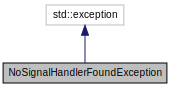
\includegraphics[width=244pt]{class_no_signal_handler_found_exception__coll__graph}
\end{center}
\end{figure}
\subsection*{Public Member Functions}
\begin{DoxyCompactItemize}
\item 
\hyperlink{class_no_signal_handler_found_exception_aedbbde0eab386ffcef936bb04da96862}{No\+Signal\+Handler\+Found\+Exception} (const std\+::string message)
\item 
\hypertarget{class_no_signal_handler_found_exception_a1d8b54d32f398d37b8e94212ec73029e}{}\label{class_no_signal_handler_found_exception_a1d8b54d32f398d37b8e94212ec73029e} 
virtual const char $\ast$ {\bfseries what} () const noexcept
\end{DoxyCompactItemize}


\subsection{Detailed Description}
\hyperlink{systemsignalhandler_8hpp_source}{systemsignalhandler.\+hpp} -\/ container for signal handlers, also handles calling of the signal handler, assumes that the handler has all the state it needs to execute.

\begin{DoxyAuthor}{Author}
\+: Jonathan Beard 
\end{DoxyAuthor}
\begin{DoxyVersion}{Version}
\+: Sat Dec 6 18\+:19\+:13 2014
\end{DoxyVersion}
Copyright 2014 Jonathan Beard

Licensed under the Apache License, Version 2.\+0 (the \char`\"{}\+License\char`\"{}); you may not use this file except in compliance with the License. You may obtain a copy of the License at\+:

\href{http://www.apache.org/licenses/LICENSE-2.0}{\tt http\+://www.\+apache.\+org/licenses/\+L\+I\+C\+E\+N\+S\+E-\/2.\+0}

Unless required by applicable law or agreed to in writing, software distributed under the License is distributed on an \char`\"{}\+A\+S I\+S\char`\"{} B\+A\+S\+IS, W\+I\+T\+H\+O\+UT W\+A\+R\+R\+A\+N\+T\+I\+ES OR C\+O\+N\+D\+I\+T\+I\+O\+NS OF A\+NY K\+I\+ND, either express or implied. See the License for the specific language governing permissions and limitations under the License. simple exception for when an exception handler is expected to be defined but actually is not. 

Definition at line 35 of file systemsignalhandler.\+hpp.



\subsection{Constructor \& Destructor Documentation}
\hypertarget{class_no_signal_handler_found_exception_aedbbde0eab386ffcef936bb04da96862}{}\label{class_no_signal_handler_found_exception_aedbbde0eab386ffcef936bb04da96862} 
\index{No\+Signal\+Handler\+Found\+Exception@{No\+Signal\+Handler\+Found\+Exception}!No\+Signal\+Handler\+Found\+Exception@{No\+Signal\+Handler\+Found\+Exception}}
\index{No\+Signal\+Handler\+Found\+Exception@{No\+Signal\+Handler\+Found\+Exception}!No\+Signal\+Handler\+Found\+Exception@{No\+Signal\+Handler\+Found\+Exception}}
\subsubsection{\texorpdfstring{No\+Signal\+Handler\+Found\+Exception()}{NoSignalHandlerFoundException()}}
{\footnotesize\ttfamily No\+Signal\+Handler\+Found\+Exception\+::\+No\+Signal\+Handler\+Found\+Exception (\begin{DoxyParamCaption}\item[{const std\+::string}]{message }\end{DoxyParamCaption})}

\hyperlink{systemsignalhandler_8cpp_source}{systemsignalhandler.\+cpp} -\/ \begin{DoxyAuthor}{Author}
\+: Jonathan Beard 
\end{DoxyAuthor}
\begin{DoxyVersion}{Version}
\+: Sat Dec 6 18\+:19\+:13 2014
\end{DoxyVersion}
Copyright 2014 Jonathan Beard

Licensed under the Apache License, Version 2.\+0 (the \char`\"{}\+License\char`\"{}); you may not use this file except in compliance with the License. You may obtain a copy of the License at\+:

\href{http://www.apache.org/licenses/LICENSE-2.0}{\tt http\+://www.\+apache.\+org/licenses/\+L\+I\+C\+E\+N\+S\+E-\/2.\+0}

Unless required by applicable law or agreed to in writing, software distributed under the License is distributed on an \char`\"{}\+A\+S I\+S\char`\"{} B\+A\+S\+IS, W\+I\+T\+H\+O\+UT W\+A\+R\+R\+A\+N\+T\+I\+ES OR C\+O\+N\+D\+I\+T\+I\+O\+NS OF A\+NY K\+I\+ND, either express or implied. See the License for the specific language governing permissions and limitations under the License. 

Definition at line 24 of file systemsignalhandler.\+cpp.



Referenced by System\+Signal\+Handler\+::call\+Handler().


\begin{DoxyCode}
26 \{
27    (\textcolor{keyword}{this})->message = message;
28 \}
\end{DoxyCode}


The documentation for this class was generated from the following files\+:\begin{DoxyCompactItemize}
\item 
systemsignalhandler.\+hpp\item 
systemsignalhandler.\+cpp\end{DoxyCompactItemize}

\hypertarget{classraft_1_1parallel__k}{}\section{raft\+:\+:parallel\+\_\+k Class Reference}
\label{classraft_1_1parallel__k}\index{raft\+::parallel\+\_\+k@{raft\+::parallel\+\_\+k}}


Inheritance diagram for raft\+:\+:parallel\+\_\+k\+:
\nopagebreak
\begin{figure}[H]
\begin{center}
\leavevmode
\includegraphics[width=159pt]{classraft_1_1parallel__k__inherit__graph}
\end{center}
\end{figure}


Collaboration diagram for raft\+:\+:parallel\+\_\+k\+:
\nopagebreak
\begin{figure}[H]
\begin{center}
\leavevmode
\includegraphics[width=350pt]{classraft_1_1parallel__k__coll__graph}
\end{center}
\end{figure}
\subsection*{Public Member Functions}
\begin{DoxyCompactItemize}
\item 
\hypertarget{classraft_1_1parallel__k_a7bc1c201f49ad35e35bffead39da7fc9}{}\label{classraft_1_1parallel__k_a7bc1c201f49ad35e35bffead39da7fc9} 
{\bfseries parallel\+\_\+k} (void $\ast$const ptr, const std\+::size\+\_\+t nbytes)
\end{DoxyCompactItemize}
\subsection*{Protected Member Functions}
\begin{DoxyCompactItemize}
\item 
{\footnotesize template$<$class T $>$ }\\std\+::size\+\_\+t \hyperlink{classraft_1_1parallel__k_a73b5ea02ddaf42293de155d0f256c854}{add\+Port\+To} (\hyperlink{class_port}{Port} \&port)
\item 
\hypertarget{classraft_1_1parallel__k_a60932e6e784dd7950d167b5d4ee5344f}{}\label{classraft_1_1parallel__k_a60932e6e784dd7950d167b5d4ee5344f} 
void {\bfseries lock\+\_\+helper} (\hyperlink{class_port}{Port} \&port)
\item 
\hypertarget{classraft_1_1parallel__k_a614bbcef8b5d5aa053e137ef4654be25}{}\label{classraft_1_1parallel__k_a614bbcef8b5d5aa053e137ef4654be25} 
void {\bfseries unlock\+\_\+helper} (\hyperlink{class_port}{Port} \&port)
\end{DoxyCompactItemize}
\subsection*{Protected Attributes}
\begin{DoxyCompactItemize}
\item 
\hypertarget{classraft_1_1parallel__k_a6cae46ace01fb33bd32147d43dda3eec}{}\label{classraft_1_1parallel__k_a6cae46ace01fb33bd32147d43dda3eec} 
std\+::size\+\_\+t {\bfseries port\+\_\+name\+\_\+index} = 0
\end{DoxyCompactItemize}
\subsection*{Friends}
\begin{DoxyCompactItemize}
\item 
\hypertarget{classraft_1_1parallel__k_a59b0d31ff28240338a2b6e682030ca3c}{}\label{classraft_1_1parallel__k_a59b0d31ff28240338a2b6e682030ca3c} 
class {\bfseries \+::\+Schedule}
\item 
\hypertarget{classraft_1_1parallel__k_aeda338414e516b47761f994fb78056c6}{}\label{classraft_1_1parallel__k_aeda338414e516b47761f994fb78056c6} 
class {\bfseries map}
\end{DoxyCompactItemize}
\subsection*{Additional Inherited Members}


\subsection{Detailed Description}


Definition at line 35 of file parallelk.\+hpp.



\subsection{Member Function Documentation}
\hypertarget{classraft_1_1parallel__k_a73b5ea02ddaf42293de155d0f256c854}{}\label{classraft_1_1parallel__k_a73b5ea02ddaf42293de155d0f256c854} 
\index{raft\+::parallel\+\_\+k@{raft\+::parallel\+\_\+k}!add\+Port\+To@{add\+Port\+To}}
\index{add\+Port\+To@{add\+Port\+To}!raft\+::parallel\+\_\+k@{raft\+::parallel\+\_\+k}}
\subsubsection{\texorpdfstring{add\+Port\+To()}{addPortTo()}}
{\footnotesize\ttfamily template$<$class T $>$ \\
std\+::size\+\_\+t raft\+::parallel\+\_\+k\+::add\+Port\+To (\begin{DoxyParamCaption}\item[{\hyperlink{class_port}{Port} \&}]{port }\end{DoxyParamCaption})\hspace{0.3cm}{\ttfamily [inline]}, {\ttfamily [protected]}}

add\+Port -\/ adds a port, either to the input or output depending on what the sub-\/class type is 

Definition at line 50 of file parallelk.\+hpp.



References Port\+::add\+Port().


\begin{DoxyCode}
51    \{
52       \textcolor{keyword}{const} \textcolor{keyword}{auto} portid( port\_name\_index++ );
53       port.\hyperlink{class_port_a9c1343a48c523fc5b285cb055ba2b53e}{addPort}< T >( std::to\_string( portid ) );
54       \textcolor{keywordflow}{return}( portid );
55    \}
\end{DoxyCode}
Here is the call graph for this function\+:
\nopagebreak
\begin{figure}[H]
\begin{center}
\leavevmode
\includegraphics[width=321pt]{classraft_1_1parallel__k_a73b5ea02ddaf42293de155d0f256c854_cgraph}
\end{center}
\end{figure}


The documentation for this class was generated from the following files\+:\begin{DoxyCompactItemize}
\item 
parallelk.\+hpp\item 
parallelk.\+cpp\end{DoxyCompactItemize}

\hypertarget{class_partition}{}\section{Partition Class Reference}
\label{class_partition}\index{Partition@{Partition}}


{\ttfamily \#include $<$partition\+\_\+old.\+hpp$>$}

\subsection*{Static Public Member Functions}
\begin{DoxyCompactItemize}
\item 
{\footnotesize template$<$class Container , class Mapping\+Container $>$ }\\static void \hyperlink{class_partition_a60481d98fd1958b78250241e6e2a011f}{simple} (Container \&c, Mapping\+Container \&mapping, const std\+::size\+\_\+t cores)
\item 
{\footnotesize template$<$class Container , class Mapping\+Container $>$ }\\static void \hyperlink{class_partition_aeb39bcc732a88f06288b38e1b1c29978}{utilization\+\_\+weighted} (Container \&c, Mapping\+Container \&mapping, const std\+::size\+\_\+t cores)
\end{DoxyCompactItemize}


\subsection{Detailed Description}
partition.\+hpp -\/ \begin{DoxyAuthor}{Author}
\+: Jonathan Beard 
\end{DoxyAuthor}
\begin{DoxyVersion}{Version}
\+: Tue Mar 10 13\+:23\+:12 2015
\end{DoxyVersion}
Copyright 2015 Jonathan Beard

Licensed under the Apache License, Version 2.\+0 (the \char`\"{}\+License\char`\"{}); you may not use this file except in compliance with the License. You may obtain a copy of the License at\+:

\href{http://www.apache.org/licenses/LICENSE-2.0}{\tt http\+://www.\+apache.\+org/licenses/\+L\+I\+C\+E\+N\+S\+E-\/2.\+0}

Unless required by applicable law or agreed to in writing, software distributed under the License is distributed on an \char`\"{}\+A\+S I\+S\char`\"{} B\+A\+S\+I\+S, W\+I\+T\+H\+O\+U\+T W\+A\+R\+R\+A\+N\+T\+I\+E\+S O\+R C\+O\+N\+D\+I\+T\+I\+O\+N\+S O\+F A\+N\+Y K\+I\+N\+D, either express or implied. See the License for the specific language governing permissions and limitations under the License.\+T\+O\+D\+O, might bring this lib into Raft\+Lib 

\subsection{Member Function Documentation}
\hypertarget{class_partition_a60481d98fd1958b78250241e6e2a011f}{}\index{Partition@{Partition}!simple@{simple}}
\index{simple@{simple}!Partition@{Partition}}
\subsubsection[{simple(\+Container \&c, Mapping\+Container \&mapping, const std\+::size\+\_\+t cores)}]{\setlength{\rightskip}{0pt plus 5cm}template$<$class Container , class Mapping\+Container $>$ static void Partition\+::simple (
\begin{DoxyParamCaption}
\item[{Container \&}]{c, }
\item[{Mapping\+Container \&}]{mapping, }
\item[{const std\+::size\+\_\+t}]{cores}
\end{DoxyParamCaption}
)\hspace{0.3cm}{\ttfamily [inline]}, {\ttfamily [static]}}\label{class_partition_a60481d98fd1958b78250241e6e2a011f}
simple weight to start \hypertarget{class_partition_aeb39bcc732a88f06288b38e1b1c29978}{}\index{Partition@{Partition}!utilization\+\_\+weighted@{utilization\+\_\+weighted}}
\index{utilization\+\_\+weighted@{utilization\+\_\+weighted}!Partition@{Partition}}
\subsubsection[{utilization\+\_\+weighted(\+Container \&c, Mapping\+Container \&mapping, const std\+::size\+\_\+t cores)}]{\setlength{\rightskip}{0pt plus 5cm}template$<$class Container , class Mapping\+Container $>$ static void Partition\+::utilization\+\_\+weighted (
\begin{DoxyParamCaption}
\item[{Container \&}]{c, }
\item[{Mapping\+Container \&}]{mapping, }
\item[{const std\+::size\+\_\+t}]{cores}
\end{DoxyParamCaption}
)\hspace{0.3cm}{\ttfamily [inline]}, {\ttfamily [static]}}\label{class_partition_aeb39bcc732a88f06288b38e1b1c29978}
else use queue weights 

The documentation for this class was generated from the following file\+:\begin{DoxyCompactItemize}
\item 
partition\+\_\+old.\+hpp\end{DoxyCompactItemize}

\hypertarget{classpool__schedule}{}\section{pool\+\_\+schedule Class Reference}
\label{classpool__schedule}\index{pool\+\_\+schedule@{pool\+\_\+schedule}}
Inheritance diagram for pool\+\_\+schedule\+:\begin{figure}[H]
\begin{center}
\leavevmode
\includegraphics[height=2.000000cm]{classpool__schedule}
\end{center}
\end{figure}
\subsection*{Public Member Functions}
\begin{DoxyCompactItemize}
\item 
\hyperlink{classpool__schedule_a11da62ac9c7b4ea203198ac3bb7babb4}{pool\+\_\+schedule} (\hyperlink{class_map}{Map} \&map)
\item 
virtual \hyperlink{classpool__schedule_a176ca5ea8ee742192b52660ecccc9290}{$\sim$pool\+\_\+schedule} ()
\item 
virtual void \hyperlink{classpool__schedule_ab67558a44404e42ba032f799c0f424a7}{start} ()
\end{DoxyCompactItemize}
\subsection*{Protected Member Functions}
\begin{DoxyCompactItemize}
\item 
virtual bool \hyperlink{classpool__schedule_aa5ec97e860a94aa17f33a0562fe942ce}{schedule\+Kernel} (\hyperlink{classraft_1_1kernel}{raft\+::kernel} $\ast$const kernel)
\end{DoxyCompactItemize}
\subsection*{Static Protected Member Functions}
\begin{DoxyCompactItemize}
\item 
static bool \hyperlink{classpool__schedule_a962f811570635fb9a9ec13c1bbcf2923}{container\+\_\+min\+\_\+input} (\hyperlink{classkernel__container}{kernel\+\_\+container} $\ast$const a, \hyperlink{classkernel__container}{kernel\+\_\+container} $\ast$const b)
\item 
static bool \hyperlink{classpool__schedule_a9cef61efbff4cd4f0b2834fa1d8448cd}{container\+\_\+min\+\_\+output} (\hyperlink{classkernel__container}{kernel\+\_\+container} $\ast$const a, \hyperlink{classkernel__container}{kernel\+\_\+container} $\ast$const b)
\end{DoxyCompactItemize}
\subsection*{Protected Attributes}
\begin{DoxyCompactItemize}
\item 
const float \hyperlink{classpool__schedule_ad58df45d8f29a1a696338a2beb058b7c}{diff\+\_\+weight} = .\+20
\item 
decltype(std\+::thread\+::hardware\+\_\+concurrency()) const \hyperlink{classpool__schedule_adc11766f8ff9a29b21318bfcf81c815d}{n\+\_\+threads}
\item 
std\+::vector$<$ std\+::thread $\ast$ $>$ \hyperlink{classpool__schedule_ae13c48902fd23d0d8747978780731a04}{pool}
\item 
std\+::vector$<$ \hyperlink{classkernel__container}{kernel\+\_\+container} $\ast$ $>$ \hyperlink{classpool__schedule_a06a6ffb1893da4d486e309f22fe3d83e}{container}
\item 
\hypertarget{classpool__schedule_a91f4b1e58cbbe08986c21d1286f3f98b}{}std\+::size\+\_\+t {\bfseries kernel\+\_\+count} = 0\label{classpool__schedule_a91f4b1e58cbbe08986c21d1286f3f98b}

\item 
\hypertarget{classpool__schedule_a7255a60e82c01a13c18ae69c8831f288}{}std\+::remove\+\_\+reference$<$ decltype(container.\+end()) $>$\+::type {\bfseries container\+\_\+it}\label{classpool__schedule_a7255a60e82c01a13c18ae69c8831f288}

\end{DoxyCompactItemize}
\subsection*{Additional Inherited Members}


\subsection{Constructor \& Destructor Documentation}
\hypertarget{classpool__schedule_a11da62ac9c7b4ea203198ac3bb7babb4}{}\index{pool\+\_\+schedule@{pool\+\_\+schedule}!pool\+\_\+schedule@{pool\+\_\+schedule}}
\index{pool\+\_\+schedule@{pool\+\_\+schedule}!pool\+\_\+schedule@{pool\+\_\+schedule}}
\subsubsection[{pool\+\_\+schedule(\+Map \&map)}]{\setlength{\rightskip}{0pt plus 5cm}pool\+\_\+schedule\+::pool\+\_\+schedule (
\begin{DoxyParamCaption}
\item[{{\bf Map} \&}]{map}
\end{DoxyParamCaption}
)}\label{classpool__schedule_a11da62ac9c7b4ea203198ac3bb7babb4}
\hyperlink{classpool__schedule}{pool\+\_\+schedule} -\/ constructor, takes a map object, calling this will launch threads. scheduler itself is also run as a thread. 
\begin{DoxyParams}{Parameters}
{\em map} & -\/ \hyperlink{class_map}{Map}\&\\
\hline
\end{DoxyParams}
poolschedule.\+cpp -\/ \begin{DoxyAuthor}{Author}
\+: Jonathan Beard 
\end{DoxyAuthor}
\begin{DoxyVersion}{Version}
\+: Thu Sep 11 15\+:49\+:57 2014
\end{DoxyVersion}
Copyright 2014 Jonathan Beard

Licensed under the Apache License, Version 2.\+0 (the \char`\"{}\+License\char`\"{}); you may not use this file except in compliance with the License. You may obtain a copy of the License at\+:

\href{http://www.apache.org/licenses/LICENSE-2.0}{\tt http\+://www.\+apache.\+org/licenses/\+L\+I\+C\+E\+N\+S\+E-\/2.\+0}

Unless required by applicable law or agreed to in writing, software distributed under the License is distributed on an \char`\"{}\+A\+S I\+S\char`\"{} B\+A\+S\+I\+S, W\+I\+T\+H\+O\+U\+T W\+A\+R\+R\+A\+N\+T\+I\+E\+S O\+R C\+O\+N\+D\+I\+T\+I\+O\+N\+S O\+F A\+N\+Y K\+I\+N\+D, either express or implied. See the License for the specific language governing permissions and limitations under the License. initialize container objects

initialize threads \hypertarget{classpool__schedule_a176ca5ea8ee742192b52660ecccc9290}{}\index{pool\+\_\+schedule@{pool\+\_\+schedule}!````~pool\+\_\+schedule@{$\sim$pool\+\_\+schedule}}
\index{````~pool\+\_\+schedule@{$\sim$pool\+\_\+schedule}!pool\+\_\+schedule@{pool\+\_\+schedule}}
\subsubsection[{$\sim$pool\+\_\+schedule()}]{\setlength{\rightskip}{0pt plus 5cm}pool\+\_\+schedule\+::$\sim$pool\+\_\+schedule (
\begin{DoxyParamCaption}
{}
\end{DoxyParamCaption}
)\hspace{0.3cm}{\ttfamily [virtual]}}\label{classpool__schedule_a176ca5ea8ee742192b52660ecccc9290}
destructor, deletes threads and cleans up container objects. join threads

delete threads

delete containers 

\subsection{Member Function Documentation}
\hypertarget{classpool__schedule_a962f811570635fb9a9ec13c1bbcf2923}{}\index{pool\+\_\+schedule@{pool\+\_\+schedule}!container\+\_\+min\+\_\+input@{container\+\_\+min\+\_\+input}}
\index{container\+\_\+min\+\_\+input@{container\+\_\+min\+\_\+input}!pool\+\_\+schedule@{pool\+\_\+schedule}}
\subsubsection[{container\+\_\+min\+\_\+input(kernel\+\_\+container $\ast$const a, kernel\+\_\+container $\ast$const b)}]{\setlength{\rightskip}{0pt plus 5cm}bool pool\+\_\+schedule\+::container\+\_\+min\+\_\+input (
\begin{DoxyParamCaption}
\item[{{\bf kernel\+\_\+container} $\ast$const}]{a, }
\item[{{\bf kernel\+\_\+container} $\ast$const}]{b}
\end{DoxyParamCaption}
)\hspace{0.3cm}{\ttfamily [static]}, {\ttfamily [protected]}}\label{classpool__schedule_a962f811570635fb9a9ec13c1bbcf2923}
container\+\_\+min -\/ returns true if the input queue of a has fewer items than the input queue of b 
\begin{DoxyParams}{Parameters}
{\em a} & -\/ \hyperlink{classkernel__container}{kernel\+\_\+container} $\ast$ const \\
\hline
{\em b} & -\/ \hyperlink{classkernel__container}{kernel\+\_\+container} $\ast$ const \\
\hline
\end{DoxyParams}
\begin{DoxyReturn}{Returns}
bool -\/ true if a-\/$>$qsize() $<$ b-\/$>$qsize() 
\end{DoxyReturn}
\hypertarget{classpool__schedule_a9cef61efbff4cd4f0b2834fa1d8448cd}{}\index{pool\+\_\+schedule@{pool\+\_\+schedule}!container\+\_\+min\+\_\+output@{container\+\_\+min\+\_\+output}}
\index{container\+\_\+min\+\_\+output@{container\+\_\+min\+\_\+output}!pool\+\_\+schedule@{pool\+\_\+schedule}}
\subsubsection[{container\+\_\+min\+\_\+output(kernel\+\_\+container $\ast$const a, kernel\+\_\+container $\ast$const b)}]{\setlength{\rightskip}{0pt plus 5cm}bool pool\+\_\+schedule\+::container\+\_\+min\+\_\+output (
\begin{DoxyParamCaption}
\item[{{\bf kernel\+\_\+container} $\ast$const}]{a, }
\item[{{\bf kernel\+\_\+container} $\ast$const}]{b}
\end{DoxyParamCaption}
)\hspace{0.3cm}{\ttfamily [static]}, {\ttfamily [protected]}}\label{classpool__schedule_a9cef61efbff4cd4f0b2834fa1d8448cd}
container\+\_\+max -\/ returns true if the output queue of a is greater than b. 
\begin{DoxyParams}{Parameters}
{\em a} & -\/ \hyperlink{classkernel__container}{kernel\+\_\+container} $\ast$ const \\
\hline
{\em b} & -\/ \hyperlink{classkernel__container}{kernel\+\_\+container} $\ast$ const \\
\hline
\end{DoxyParams}
\begin{DoxyReturn}{Returns}
bool -\/ true if a-\/$>$outqsize $>$ b-\/$>$qoutsize 
\end{DoxyReturn}
\hypertarget{classpool__schedule_aa5ec97e860a94aa17f33a0562fe942ce}{}\index{pool\+\_\+schedule@{pool\+\_\+schedule}!schedule\+Kernel@{schedule\+Kernel}}
\index{schedule\+Kernel@{schedule\+Kernel}!pool\+\_\+schedule@{pool\+\_\+schedule}}
\subsubsection[{schedule\+Kernel(raft\+::kernel $\ast$const kernel)}]{\setlength{\rightskip}{0pt plus 5cm}bool pool\+\_\+schedule\+::schedule\+Kernel (
\begin{DoxyParamCaption}
\item[{{\bf raft\+::kernel} $\ast$const}]{kernel}
\end{DoxyParamCaption}
)\hspace{0.3cm}{\ttfamily [protected]}, {\ttfamily [virtual]}}\label{classpool__schedule_aa5ec97e860a94aa17f33a0562fe942ce}
B\+E\+G\+I\+N F\+U\+N\+C\+T\+I\+O\+N\+S schedule\+Kernel -\/ override base class function in order to add kernels to the right place. 
\begin{DoxyParams}{Parameters}
{\em kernel} & -\/ \hyperlink{classraft_1_1kernel}{raft\+::kernel}$\ast$ \\
\hline
\end{DoxyParams}
\begin{DoxyReturn}{Returns}
bool -\/ always true 
\end{DoxyReturn}
get a container \hypertarget{classpool__schedule_ab67558a44404e42ba032f799c0f424a7}{}\index{pool\+\_\+schedule@{pool\+\_\+schedule}!start@{start}}
\index{start@{start}!pool\+\_\+schedule@{pool\+\_\+schedule}}
\subsubsection[{start()}]{\setlength{\rightskip}{0pt plus 5cm}void pool\+\_\+schedule\+::start (
\begin{DoxyParamCaption}
{}
\end{DoxyParamCaption}
)\hspace{0.3cm}{\ttfamily [virtual]}}\label{classpool__schedule_ab67558a44404e42ba032f799c0f424a7}
start -\/ call to start executing map, at this point the mapper sould have checked the topology and everything should be set up for running. we want to get the max queue occupancy

some message exists

remove kernel

all done, shutdown 

Implements \hyperlink{class_schedule_ab6ad5540ecdef6b472b4e8242a47c4ee}{Schedule}.



\subsection{Member Data Documentation}
\hypertarget{classpool__schedule_a06a6ffb1893da4d486e309f22fe3d83e}{}\index{pool\+\_\+schedule@{pool\+\_\+schedule}!container@{container}}
\index{container@{container}!pool\+\_\+schedule@{pool\+\_\+schedule}}
\subsubsection[{container}]{\setlength{\rightskip}{0pt plus 5cm}std\+::vector$<$ {\bf kernel\+\_\+container}$\ast$ $>$ pool\+\_\+schedule\+::container\hspace{0.3cm}{\ttfamily [protected]}}\label{classpool__schedule_a06a6ffb1893da4d486e309f22fe3d83e}
max\+\_\+heap\+\_\+container -\/ sorted by max output-\/queue occupancy \hypertarget{classpool__schedule_ad58df45d8f29a1a696338a2beb058b7c}{}\index{pool\+\_\+schedule@{pool\+\_\+schedule}!diff\+\_\+weight@{diff\+\_\+weight}}
\index{diff\+\_\+weight@{diff\+\_\+weight}!pool\+\_\+schedule@{pool\+\_\+schedule}}
\subsubsection[{diff\+\_\+weight}]{\setlength{\rightskip}{0pt plus 5cm}const float pool\+\_\+schedule\+::diff\+\_\+weight = .\+20\hspace{0.3cm}{\ttfamily [protected]}}\label{classpool__schedule_ad58df45d8f29a1a696338a2beb058b7c}
E\+N\+D F\+U\+N\+C\+T\+I\+O\+N\+S, B\+E\+G\+I\+N V\+A\+R D\+E\+C\+L\+S The thread has to have this much more \char`\"{}work\char`\"{} than the previous thread in order to get moved ot a new thread. Used in \hyperlink{classpool__schedule_ab67558a44404e42ba032f799c0f424a7}{pool\+\_\+schedule\+::start()}. \hypertarget{classpool__schedule_adc11766f8ff9a29b21318bfcf81c815d}{}\index{pool\+\_\+schedule@{pool\+\_\+schedule}!n\+\_\+threads@{n\+\_\+threads}}
\index{n\+\_\+threads@{n\+\_\+threads}!pool\+\_\+schedule@{pool\+\_\+schedule}}
\subsubsection[{n\+\_\+threads}]{\setlength{\rightskip}{0pt plus 5cm}decltype( std\+::thread\+::hardware\+\_\+concurrency() ) const pool\+\_\+schedule\+::n\+\_\+threads\hspace{0.3cm}{\ttfamily [protected]}}\label{classpool__schedule_adc11766f8ff9a29b21318bfcf81c815d}
total \# of hardware supported threads \hypertarget{classpool__schedule_ae13c48902fd23d0d8747978780731a04}{}\index{pool\+\_\+schedule@{pool\+\_\+schedule}!pool@{pool}}
\index{pool@{pool}!pool\+\_\+schedule@{pool\+\_\+schedule}}
\subsubsection[{pool}]{\setlength{\rightskip}{0pt plus 5cm}std\+::vector$<$ std\+::thread$\ast$ $>$ pool\+\_\+schedule\+::pool\hspace{0.3cm}{\ttfamily [protected]}}\label{classpool__schedule_ae13c48902fd23d0d8747978780731a04}
used as a thread pool 

The documentation for this class was generated from the following files\+:\begin{DoxyCompactItemize}
\item 
poolschedule.\+hpp\item 
poolschedule.\+cpp\end{DoxyCompactItemize}

\hypertarget{class_port}{}\section{Port Class Reference}
\label{class_port}\index{Port@{Port}}
Inheritance diagram for Port\+:\begin{figure}[H]
\begin{center}
\leavevmode
\includegraphics[height=2.000000cm]{class_port}
\end{center}
\end{figure}
\subsection*{Public Member Functions}
\begin{DoxyCompactItemize}
\item 
\hyperlink{class_port_ac7da4ae14a771d5509e743e98fe0dc05}{Port} (\hyperlink{classraft_1_1kernel}{raft\+::kernel} $\ast$k)
\item 
\hyperlink{class_port_a706968dde40372ffd1748d50c258f6b7}{Port} (\hyperlink{classraft_1_1kernel}{raft\+::kernel} $\ast$k, void $\ast$const ptr, const std\+::size\+\_\+t nbytes)
\item 
virtual \hyperlink{class_port_afe166c2a6b10ad34d47472a150366bc1}{$\sim$\+Port} ()
\item 
{\footnotesize template$<$class T $>$ }\\void \hyperlink{class_port_aeb1c43cc7563ce977ba0bc7b581d2e75}{add\+Port} (const std\+::string \&\&port\+\_\+name)
\item 
{\footnotesize template$<$class T $>$ }\\bool \hyperlink{class_port_aaf89e298b9ae64f9c42703c14d9eed0a}{add\+In\+Place\+Ports} (const std\+::size\+\_\+t n\+\_\+ports)
\item 
const std\+::type\+\_\+index \& \hyperlink{class_port_af34969d8f5e17ad29233334526d5b77b}{get\+Port\+Type} (const std\+::string \&\&port\+\_\+name)
\item 
virtual F\+I\+F\+O \& \hyperlink{class_port_a08cf165426982d83e5a191ba74cc6e5d}{operator\mbox{[}$\,$\mbox{]}} (const std\+::string \&\&port\+\_\+name)
\item 
virtual bool \hyperlink{class_port_a7042f5b5c2ab14c9591a4984811a6012}{has\+Ports} ()
\item 
virtual \hyperlink{class_port_iterator}{Port\+Iterator} \hyperlink{class_port_abf4d86026b67f6c02db3e3abb0f2e8b4}{begin} ()
\item 
virtual \hyperlink{class_port_iterator}{Port\+Iterator} \hyperlink{class_port_aa85be3fb7734863d482bf002e0f0923d}{end} ()
\item 
std\+::size\+\_\+t \hyperlink{class_port_a33562ea87ac7e83a32441da40cbd9279}{count} ()
\end{DoxyCompactItemize}
\subsection*{Protected Member Functions}
\begin{DoxyCompactItemize}
\item 
{\footnotesize template$<$class T $>$ }\\void \hyperlink{class_port_a90a9a883b2e10871e7a8dc55ab0077f5}{initialize\+Const\+Map} (\hyperlink{struct_port_info}{Port\+Info} \&pi)
\item 
{\footnotesize template$<$class T $>$ }\\void \hyperlink{class_port_a7189f6823a0d240396210a7c317d4803}{initialize\+Split} (\hyperlink{struct_port_info}{Port\+Info} \&pi)
\item 
{\footnotesize template$<$class T $>$ }\\void \hyperlink{class_port_a179c9a36189eb621a5874a0741708e59}{initialize\+Join} (\hyperlink{struct_port_info}{Port\+Info} \&pi)
\item 
\hyperlink{struct_port_info}{Port\+Info} \& \hyperlink{class_port_a4af1cb062940ca3b83c569f024b9a8d1}{get\+Port\+Info} ()
\item 
\hyperlink{struct_port_info}{Port\+Info} \& \hyperlink{class_port_afb426a015195fa9b4b5b1d1200daf8ed}{get\+Port\+Info\+For} (const std\+::string port\+\_\+name)
\end{DoxyCompactItemize}
\subsection*{Protected Attributes}
\begin{DoxyCompactItemize}
\item 
\hyperlink{structportmap__t}{portmap\+\_\+t} \hyperlink{class_port_a537a8a0c2a47acbf8654f286200aee90}{portmap}
\item 
\hyperlink{classraft_1_1kernel}{raft\+::kernel} $\ast$ \hyperlink{class_port_ac17060db235459adaab87cdccb605884}{kernel} = nullptr
\item 
void $\ast$const \hyperlink{class_port_a78bf16e68f1dd5312f37b4e2806a9cf8}{alloc\+\_\+ptr} = nullptr
\item 
const std\+::size\+\_\+t \hyperlink{class_port_a98d2e7e0e570e082465c692083300fa9}{alloc\+\_\+ptr\+\_\+length} = 0
\end{DoxyCompactItemize}
\subsection*{Friends}
\begin{DoxyCompactItemize}
\item 
class \hyperlink{class_port_aed45534b6a99d5630dcfa9eedbe023fc}{Map\+Base}
\item 
\hypertarget{class_port_ad2f32e921244459f7cc6d50355429cc6}{}class {\bfseries Map}\label{class_port_ad2f32e921244459f7cc6d50355429cc6}

\item 
\hypertarget{class_port_a60770fd1bd2e4378b64b8bb78b3af209}{}class {\bfseries Graph\+Tools}\label{class_port_a60770fd1bd2e4378b64b8bb78b3af209}

\item 
\hypertarget{class_port_a901ac6fe1c35f3c114cf9e83f75dde0c}{}class {\bfseries basic\+\_\+parallel}\label{class_port_a901ac6fe1c35f3c114cf9e83f75dde0c}

\item 
\hypertarget{class_port_abf9ffb5a15eb9623a47ea7e488ae112b}{}class {\bfseries raft\+::parallel\+\_\+k}\label{class_port_abf9ffb5a15eb9623a47ea7e488ae112b}

\end{DoxyCompactItemize}


\subsection{Constructor \& Destructor Documentation}
\hypertarget{class_port_ac7da4ae14a771d5509e743e98fe0dc05}{}\index{Port@{Port}!Port@{Port}}
\index{Port@{Port}!Port@{Port}}
\subsubsection[{Port(raft\+::kernel $\ast$k)}]{\setlength{\rightskip}{0pt plus 5cm}Port\+::\+Port (
\begin{DoxyParamCaption}
\item[{{\bf raft\+::kernel} $\ast$}]{k}
\end{DoxyParamCaption}
)}\label{class_port_ac7da4ae14a771d5509e743e98fe0dc05}
\hyperlink{class_port}{Port} -\/ constructor used to construct a standard port object, needs a reference to the parent kernel for the port\+\_\+info struct 
\begin{DoxyParams}{Parameters}
{\em k} & -\/ \hyperlink{classraft_1_1kernel}{raft\+::kernel}$\ast$\\
\hline
\end{DoxyParams}
port.\+cpp -\/ \begin{DoxyAuthor}{Author}
\+: Jonathan Beard 
\end{DoxyAuthor}
\begin{DoxyVersion}{Version}
\+: Thu Aug 28 09\+:55\+:47 2014
\end{DoxyVersion}
Copyright 2014 Jonathan Beard

Licensed under the Apache License, Version 2.\+0 (the \char`\"{}\+License\char`\"{}); you may not use this file except in compliance with the License. You may obtain a copy of the License at\+:

\href{http://www.apache.org/licenses/LICENSE-2.0}{\tt http\+://www.\+apache.\+org/licenses/\+L\+I\+C\+E\+N\+S\+E-\/2.\+0}

Unless required by applicable law or agreed to in writing, software distributed under the License is distributed on an \char`\"{}\+A\+S I\+S\char`\"{} B\+A\+S\+I\+S, W\+I\+T\+H\+O\+U\+T W\+A\+R\+R\+A\+N\+T\+I\+E\+S O\+R C\+O\+N\+D\+I\+T\+I\+O\+N\+S O\+F A\+N\+Y K\+I\+N\+D, either express or implied. See the License for the specific language governing permissions and limitations under the License. \hypertarget{class_port_a706968dde40372ffd1748d50c258f6b7}{}\index{Port@{Port}!Port@{Port}}
\index{Port@{Port}!Port@{Port}}
\subsubsection[{Port(raft\+::kernel $\ast$k, void $\ast$const ptr, const std\+::size\+\_\+t nbytes)}]{\setlength{\rightskip}{0pt plus 5cm}Port\+::\+Port (
\begin{DoxyParamCaption}
\item[{{\bf raft\+::kernel} $\ast$}]{k, }
\item[{void $\ast$const}]{ptr, }
\item[{const std\+::size\+\_\+t}]{nbytes}
\end{DoxyParamCaption}
)}\label{class_port_a706968dde40372ffd1748d50c258f6b7}
\hyperlink{class_port}{Port} -\/ constructor used to construct a port with pre-\/allocated memory, useful for things like array distribution and reduction 
\begin{DoxyParams}{Parameters}
{\em k} & -\/ \hyperlink{classraft_1_1kernel}{raft\+::kernel}$\ast$ \\
\hline
{\em ptr} & -\/ void$\ast$ \\
\hline
{\em nbytes} & -\/ const std\+::size\+\_\+t length in bytes \\
\hline
\end{DoxyParams}
\hypertarget{class_port_afe166c2a6b10ad34d47472a150366bc1}{}\index{Port@{Port}!````~Port@{$\sim$\+Port}}
\index{````~Port@{$\sim$\+Port}!Port@{Port}}
\subsubsection[{$\sim$\+Port()}]{\setlength{\rightskip}{0pt plus 5cm}Port\+::$\sim$\+Port (
\begin{DoxyParamCaption}
{}
\end{DoxyParamCaption}
)\hspace{0.3cm}{\ttfamily [virtual]}}\label{class_port_afe166c2a6b10ad34d47472a150366bc1}
$\sim$\+Port -\/ destructor, deletes the F\+I\+F\+O that was given when the object was initalized. the port map is allocated on the heap so the port\+\_\+info destructor is called

\subsection{Member Function Documentation}
\hypertarget{class_port_aaf89e298b9ae64f9c42703c14d9eed0a}{}\index{Port@{Port}!add\+In\+Place\+Ports@{add\+In\+Place\+Ports}}
\index{add\+In\+Place\+Ports@{add\+In\+Place\+Ports}!Port@{Port}}
\subsubsection[{add\+In\+Place\+Ports(const std\+::size\+\_\+t n\+\_\+ports)}]{\setlength{\rightskip}{0pt plus 5cm}template$<$class T $>$ bool Port\+::add\+In\+Place\+Ports (
\begin{DoxyParamCaption}
\item[{const std\+::size\+\_\+t}]{n\+\_\+ports}
\end{DoxyParamCaption}
)\hspace{0.3cm}{\ttfamily [inline]}}\label{class_port_aaf89e298b9ae64f9c42703c14d9eed0a}
add\+Ports -\/ add ports for an existing buffer, basically allocate buffers in place. These also won\textquotesingle{}t be able to be resized. 
\begin{DoxyParams}{Parameters}
{\em n\+\_\+ports} & -\/ const std\+::size\+\_\+t \\
\hline
\end{DoxyParams}
pointer \hypertarget{class_port_aeb1c43cc7563ce977ba0bc7b581d2e75}{}\index{Port@{Port}!add\+Port@{add\+Port}}
\index{add\+Port@{add\+Port}!Port@{Port}}
\subsubsection[{add\+Port(const std\+::string \&\&port\+\_\+name)}]{\setlength{\rightskip}{0pt plus 5cm}template$<$class T $>$ void Port\+::add\+Port (
\begin{DoxyParamCaption}
\item[{const std\+::string \&\&}]{port\+\_\+name}
\end{DoxyParamCaption}
)\hspace{0.3cm}{\ttfamily [inline]}}\label{class_port_aeb1c43cc7563ce977ba0bc7b581d2e75}
add\+Port -\/ adds and initializes a port for the name given. Function returns true if added, false if not. Main reason for returning false would be that the port already exists. 
\begin{DoxyParams}{Parameters}
{\em port\+\_\+name} & -\/ const std\+::string \\
\hline
\end{DoxyParams}
\begin{DoxyReturn}{Returns}
bool 
\end{DoxyReturn}
we\textquotesingle{}ll have to make a port info object first and pass it by copy to the portmap. Perhaps re-\/work later with pointers, but for right now this will work and it doesn\textquotesingle{}t necessarily have to be performant since its only executed once.\hypertarget{class_port_abf4d86026b67f6c02db3e3abb0f2e8b4}{}\index{Port@{Port}!begin@{begin}}
\index{begin@{begin}!Port@{Port}}
\subsubsection[{begin()}]{\setlength{\rightskip}{0pt plus 5cm}{\bf Port\+Iterator} Port\+::begin (
\begin{DoxyParamCaption}
{}
\end{DoxyParamCaption}
)\hspace{0.3cm}{\ttfamily [virtual]}}\label{class_port_abf4d86026b67f6c02db3e3abb0f2e8b4}
begin -\/ get the beginning port. \begin{DoxyReturn}{Returns}
\hyperlink{class_port_iterator}{Port\+Iterator} 
\end{DoxyReturn}


Implements \hyperlink{class_port_base_afc54c92e3b9d1967e8a8c7e74d7507d3}{Port\+Base}.

\hypertarget{class_port_a33562ea87ac7e83a32441da40cbd9279}{}\index{Port@{Port}!count@{count}}
\index{count@{count}!Port@{Port}}
\subsubsection[{count()}]{\setlength{\rightskip}{0pt plus 5cm}std\+::size\+\_\+t Port\+::count (
\begin{DoxyParamCaption}
{}
\end{DoxyParamCaption}
)}\label{class_port_a33562ea87ac7e83a32441da40cbd9279}
count -\/ get the total number of fifos within this port container \begin{DoxyReturn}{Returns}
std\+::size\+\_\+t 
\end{DoxyReturn}
\hypertarget{class_port_aa85be3fb7734863d482bf002e0f0923d}{}\index{Port@{Port}!end@{end}}
\index{end@{end}!Port@{Port}}
\subsubsection[{end()}]{\setlength{\rightskip}{0pt plus 5cm}{\bf Port\+Iterator} Port\+::end (
\begin{DoxyParamCaption}
{}
\end{DoxyParamCaption}
)\hspace{0.3cm}{\ttfamily [virtual]}}\label{class_port_aa85be3fb7734863d482bf002e0f0923d}
end -\/ get the end port \begin{DoxyReturn}{Returns}
\hyperlink{class_port_iterator}{Port\+Iterator} 
\end{DoxyReturn}


Implements \hyperlink{class_port_base_a50427e7a1beea0d5111ccc81ee418178}{Port\+Base}.

\hypertarget{class_port_a4af1cb062940ca3b83c569f024b9a8d1}{}\index{Port@{Port}!get\+Port\+Info@{get\+Port\+Info}}
\index{get\+Port\+Info@{get\+Port\+Info}!Port@{Port}}
\subsubsection[{get\+Port\+Info()}]{\setlength{\rightskip}{0pt plus 5cm}{\bf Port\+Info} \& Port\+::get\+Port\+Info (
\begin{DoxyParamCaption}
{}
\end{DoxyParamCaption}
)\hspace{0.3cm}{\ttfamily [protected]}}\label{class_port_a4af1cb062940ca3b83c569f024b9a8d1}
get\+Port\+Info -\/ returns the \hyperlink{struct_port_info}{Port\+Info} struct for a kernel if we expect it to have a single port. If there\textquotesingle{}s more than one port this function throws an exception. \begin{DoxyReturn}{Returns}
std\+::pair$<$ std\+::string, Port\+Info\& $>$ 
\end{DoxyReturn}
T\+O\+D\+O\+: extract kernel name to go here too \hypertarget{class_port_afb426a015195fa9b4b5b1d1200daf8ed}{}\index{Port@{Port}!get\+Port\+Info\+For@{get\+Port\+Info\+For}}
\index{get\+Port\+Info\+For@{get\+Port\+Info\+For}!Port@{Port}}
\subsubsection[{get\+Port\+Info\+For(const std\+::string port\+\_\+name)}]{\setlength{\rightskip}{0pt plus 5cm}{\bf Port\+Info} \& Port\+::get\+Port\+Info\+For (
\begin{DoxyParamCaption}
\item[{const std\+::string}]{port\+\_\+name}
\end{DoxyParamCaption}
)\hspace{0.3cm}{\ttfamily [protected]}}\label{class_port_afb426a015195fa9b4b5b1d1200daf8ed}
get\+Port\+Info\+For -\/ gets port information for the param port throws an exception if the port doesn\textquotesingle{}t exist. 
\begin{DoxyParams}{Parameters}
{\em port\+\_\+name} & -\/ const std\+::string \\
\hline
\end{DoxyParams}
\begin{DoxyReturn}{Returns}
\hyperlink{struct_port_info}{Port\+Info}\& 
\end{DoxyReturn}
\hypertarget{class_port_af34969d8f5e17ad29233334526d5b77b}{}\index{Port@{Port}!get\+Port\+Type@{get\+Port\+Type}}
\index{get\+Port\+Type@{get\+Port\+Type}!Port@{Port}}
\subsubsection[{get\+Port\+Type(const std\+::string \&\&port\+\_\+name)}]{\setlength{\rightskip}{0pt plus 5cm}const std\+::type\+\_\+index \& Port\+::get\+Port\+Type (
\begin{DoxyParamCaption}
\item[{const std\+::string \&\&}]{port\+\_\+name}
\end{DoxyParamCaption}
)}\label{class_port_af34969d8f5e17ad29233334526d5b77b}
get\+Port\+Type -\/ input the port name, and get the hash for the type of the port. This function is useful for checking the streaming graph to make sure all the ports that are \char`\"{}dynamically\char`\"{} created do in fact have compatible types. 
\begin{DoxyParams}{Parameters}
{\em port\+\_\+name} & -\/ const std\+::string \\
\hline
\end{DoxyParams}
\begin{DoxyReturn}{Returns}
const type\+\_\+index\& 
\end{DoxyReturn}

\begin{DoxyExceptions}{Exceptions}
{\em \hyperlink{class_port_not_found_exception}{Port\+Not\+Found\+Exception}} & \\
\hline
\end{DoxyExceptions}
\hypertarget{class_port_a7042f5b5c2ab14c9591a4984811a6012}{}\index{Port@{Port}!has\+Ports@{has\+Ports}}
\index{has\+Ports@{has\+Ports}!Port@{Port}}
\subsubsection[{has\+Ports()}]{\setlength{\rightskip}{0pt plus 5cm}bool Port\+::has\+Ports (
\begin{DoxyParamCaption}
{}
\end{DoxyParamCaption}
)\hspace{0.3cm}{\ttfamily [virtual]}}\label{class_port_a7042f5b5c2ab14c9591a4984811a6012}
has\+Ports -\/ returns true if any ports exists, false otherwise. \begin{DoxyReturn}{Returns}
bool 
\end{DoxyReturn}


Implements \hyperlink{class_port_base_a29870b5e201f46a806d2269d7f4635dc}{Port\+Base}.

\hypertarget{class_port_a90a9a883b2e10871e7a8dc55ab0077f5}{}\index{Port@{Port}!initialize\+Const\+Map@{initialize\+Const\+Map}}
\index{initialize\+Const\+Map@{initialize\+Const\+Map}!Port@{Port}}
\subsubsection[{initialize\+Const\+Map(\+Port\+Info \&pi)}]{\setlength{\rightskip}{0pt plus 5cm}template$<$class T $>$ void Port\+::initialize\+Const\+Map (
\begin{DoxyParamCaption}
\item[{{\bf Port\+Info} \&}]{pi}
\end{DoxyParamCaption}
)\hspace{0.3cm}{\ttfamily [inline]}, {\ttfamily [protected]}}\label{class_port_a90a9a883b2e10871e7a8dc55ab0077f5}
initialize\+Const\+Map -\/ hack to get around the inability to otherwise initialize a template function where later we don\textquotesingle{}t have the template parameter. N\+O\+T\+E\+: this is a biggy, if we have more F\+I\+F\+O types in the future (i.\+e., sub-\/classes of F\+I\+F\+O) then we must create an entry here otherwise bad things will happen. 
\begin{DoxyParams}{Parameters}
{\em pi} & -\/ \hyperlink{struct_port_info}{Port\+Info}\& \\
\hline
\end{DoxyParams}
no instrumentation

yes instrumentation

no instrumentation

N\+O\+T\+E\+: If you define more port resource types, they have to be defined here...otherwise the allocator won\textquotesingle{}t be able to allocate the correct type, size, etc. for the port..and well, it\textquotesingle{}ll be sad.\hypertarget{class_port_a179c9a36189eb621a5874a0741708e59}{}\index{Port@{Port}!initialize\+Join@{initialize\+Join}}
\index{initialize\+Join@{initialize\+Join}!Port@{Port}}
\subsubsection[{initialize\+Join(\+Port\+Info \&pi)}]{\setlength{\rightskip}{0pt plus 5cm}template$<$class T $>$ void Port\+::initialize\+Join (
\begin{DoxyParamCaption}
\item[{{\bf Port\+Info} \&}]{pi}
\end{DoxyParamCaption}
)\hspace{0.3cm}{\ttfamily [inline]}, {\ttfamily [protected]}}\label{class_port_a179c9a36189eb621a5874a0741708e59}
initialize\+Join -\/ pre-\/allocate join kernels...saves allocation time later, takes up minimal space and all that is needed when these are actually used is to allocate memory for the ports which is done by the \hypertarget{class_port_a7189f6823a0d240396210a7c317d4803}{}\index{Port@{Port}!initialize\+Split@{initialize\+Split}}
\index{initialize\+Split@{initialize\+Split}!Port@{Port}}
\subsubsection[{initialize\+Split(\+Port\+Info \&pi)}]{\setlength{\rightskip}{0pt plus 5cm}template$<$class T $>$ void Port\+::initialize\+Split (
\begin{DoxyParamCaption}
\item[{{\bf Port\+Info} \&}]{pi}
\end{DoxyParamCaption}
)\hspace{0.3cm}{\ttfamily [inline]}, {\ttfamily [protected]}}\label{class_port_a7189f6823a0d240396210a7c317d4803}
initialize\+Split -\/ pre-\/allocate split kernels...saves allocation time later, then all that is needed is to hook them up, and allocate memory for the ports. \hypertarget{class_port_a08cf165426982d83e5a191ba74cc6e5d}{}\index{Port@{Port}!operator\mbox{[}$\,$\mbox{]}@{operator[]}}
\index{operator\mbox{[}$\,$\mbox{]}@{operator[]}!Port@{Port}}
\subsubsection[{operator[](const std\+::string \&\&port\+\_\+name)}]{\setlength{\rightskip}{0pt plus 5cm}F\+I\+F\+O \& Port\+::operator\mbox{[}$\,$\mbox{]} (
\begin{DoxyParamCaption}
\item[{const std\+::string \&\&}]{port\+\_\+name}
\end{DoxyParamCaption}
)\hspace{0.3cm}{\ttfamily [virtual]}}\label{class_port_a08cf165426982d83e5a191ba74cc6e5d}
operator\mbox{[}\mbox{]} -\/ input the port name and get a port if it exists. 

Implements \hyperlink{class_port_base_ad034502b053f3cd7939d651b2d72cd0a}{Port\+Base}.



\subsection{Friends And Related Function Documentation}
\hypertarget{class_port_aed45534b6a99d5630dcfa9eedbe023fc}{}\index{Port@{Port}!Map\+Base@{Map\+Base}}
\index{Map\+Base@{Map\+Base}!Port@{Port}}
\subsubsection[{Map\+Base}]{\setlength{\rightskip}{0pt plus 5cm}friend class {\bf Map\+Base}\hspace{0.3cm}{\ttfamily [friend]}}\label{class_port_aed45534b6a99d5630dcfa9eedbe023fc}
we need some friends 

\subsection{Member Data Documentation}
\hypertarget{class_port_a78bf16e68f1dd5312f37b4e2806a9cf8}{}\index{Port@{Port}!alloc\+\_\+ptr@{alloc\+\_\+ptr}}
\index{alloc\+\_\+ptr@{alloc\+\_\+ptr}!Port@{Port}}
\subsubsection[{alloc\+\_\+ptr}]{\setlength{\rightskip}{0pt plus 5cm}void$\ast$ const Port\+::alloc\+\_\+ptr = nullptr\hspace{0.3cm}{\ttfamily [protected]}}\label{class_port_a78bf16e68f1dd5312f37b4e2806a9cf8}
ptr used for in-\/place allocations, will not be deleted by the map, also should not be modified by the map either. \hypertarget{class_port_a98d2e7e0e570e082465c692083300fa9}{}\index{Port@{Port}!alloc\+\_\+ptr\+\_\+length@{alloc\+\_\+ptr\+\_\+length}}
\index{alloc\+\_\+ptr\+\_\+length@{alloc\+\_\+ptr\+\_\+length}!Port@{Port}}
\subsubsection[{alloc\+\_\+ptr\+\_\+length}]{\setlength{\rightskip}{0pt plus 5cm}const std\+::size\+\_\+t Port\+::alloc\+\_\+ptr\+\_\+length = 0\hspace{0.3cm}{\ttfamily [protected]}}\label{class_port_a98d2e7e0e570e082465c692083300fa9}
alloc\+\_\+ptr\+\_\+length -\/ length of alloc\+\_\+ptr in bytes. \hypertarget{class_port_ac17060db235459adaab87cdccb605884}{}\index{Port@{Port}!kernel@{kernel}}
\index{kernel@{kernel}!Port@{Port}}
\subsubsection[{kernel}]{\setlength{\rightskip}{0pt plus 5cm}{\bf raft\+::kernel}$\ast$ Port\+::kernel = nullptr\hspace{0.3cm}{\ttfamily [protected]}}\label{class_port_ac17060db235459adaab87cdccb605884}
parent kernel that owns this port \hypertarget{class_port_a537a8a0c2a47acbf8654f286200aee90}{}\index{Port@{Port}!portmap@{portmap}}
\index{portmap@{portmap}!Port@{Port}}
\subsubsection[{portmap}]{\setlength{\rightskip}{0pt plus 5cm}{\bf portmap\+\_\+t} Port\+::portmap\hspace{0.3cm}{\ttfamily [protected]}}\label{class_port_a537a8a0c2a47acbf8654f286200aee90}
portmap -\/ container struct with all ports. The mutex should be locked before accessing this structure 

The documentation for this class was generated from the following files\+:\begin{DoxyCompactItemize}
\item 
port.\+hpp\item 
port.\+cpp\end{DoxyCompactItemize}

\hypertarget{class_port_already_exists}{}\section{Port\+Already\+Exists Class Reference}
\label{class_port_already_exists}\index{Port\+Already\+Exists@{Port\+Already\+Exists}}
Inheritance diagram for Port\+Already\+Exists\+:\begin{figure}[H]
\begin{center}
\leavevmode
\includegraphics[height=3.000000cm]{class_port_already_exists}
\end{center}
\end{figure}
\subsection*{Public Member Functions}
\begin{DoxyCompactItemize}
\item 
\hypertarget{class_port_already_exists_a50454163ba6c3315685b4f82f54df6d3}{}{\bfseries Port\+Already\+Exists} (const std\+::string message)\label{class_port_already_exists_a50454163ba6c3315685b4f82f54df6d3}

\end{DoxyCompactItemize}


The documentation for this class was generated from the following files\+:\begin{DoxyCompactItemize}
\item 
portexception.\+hpp\item 
portexception.\+cpp\end{DoxyCompactItemize}

\hypertarget{class_port_base}{}\section{Port\+Base Class Reference}
\label{class_port_base}\index{Port\+Base@{Port\+Base}}


{\ttfamily \#include $<$portbase.\+hpp$>$}



Inheritance diagram for Port\+Base\+:
\nopagebreak
\begin{figure}[H]
\begin{center}
\leavevmode
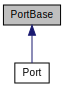
\includegraphics[width=137pt]{class_port_base__inherit__graph}
\end{center}
\end{figure}
\subsection*{Public Member Functions}
\begin{DoxyCompactItemize}
\item 
virtual \hyperlink{class_f_i_f_o}{F\+I\+FO} \& \hyperlink{class_port_base_ad034502b053f3cd7939d651b2d72cd0a}{operator\mbox{[}$\,$\mbox{]}} (const std\+::string \&\&port\+\_\+name)=0
\item 
virtual bool \hyperlink{class_port_base_a29870b5e201f46a806d2269d7f4635dc}{has\+Ports} ()=0
\item 
virtual \hyperlink{class_port_iterator}{Port\+Iterator} \hyperlink{class_port_base_afc54c92e3b9d1967e8a8c7e74d7507d3}{begin} ()=0
\item 
virtual \hyperlink{class_port_iterator}{Port\+Iterator} \hyperlink{class_port_base_a50427e7a1beea0d5111ccc81ee418178}{end} ()=0
\end{DoxyCompactItemize}


\subsection{Detailed Description}
\hyperlink{portbase_8hpp_source}{portbase.\+hpp} -\/ Interface for port types. Ensures that all port sub-\/classes have at least the functions listed below.

\begin{DoxyAuthor}{Author}
\+: Jonathan Beard 
\end{DoxyAuthor}
\begin{DoxyVersion}{Version}
\+: Sun Nov 30 10\+:22\+:46 2014
\end{DoxyVersion}
Copyright 2014 Jonathan Beard

Licensed under the Apache License, Version 2.\+0 (the \char`\"{}\+License\char`\"{}); you may not use this file except in compliance with the License. You may obtain a copy of the License at\+:

\href{http://www.apache.org/licenses/LICENSE-2.0}{\tt http\+://www.\+apache.\+org/licenses/\+L\+I\+C\+E\+N\+S\+E-\/2.\+0}

Unless required by applicable law or agreed to in writing, software distributed under the License is distributed on an \char`\"{}\+A\+S I\+S\char`\"{} B\+A\+S\+IS, W\+I\+T\+H\+O\+UT W\+A\+R\+R\+A\+N\+T\+I\+ES OR C\+O\+N\+D\+I\+T\+I\+O\+NS OF A\+NY K\+I\+ND, either express or implied. See the License for the specific language governing permissions and limitations under the License. 

Definition at line 28 of file portbase.\+hpp.



\subsection{Member Function Documentation}
\hypertarget{class_port_base_afc54c92e3b9d1967e8a8c7e74d7507d3}{}\label{class_port_base_afc54c92e3b9d1967e8a8c7e74d7507d3} 
\index{Port\+Base@{Port\+Base}!begin@{begin}}
\index{begin@{begin}!Port\+Base@{Port\+Base}}
\subsubsection{\texorpdfstring{begin()}{begin()}}
{\footnotesize\ttfamily virtual \hyperlink{class_port_iterator}{Port\+Iterator} Port\+Base\+::begin (\begin{DoxyParamCaption}{ }\end{DoxyParamCaption})\hspace{0.3cm}{\ttfamily [pure virtual]}}

begin -\/ returns a forward iterator to the port list, implementations should be thread safe so that auto-\/ parallelized code can function properly. \begin{DoxyReturn}{Returns}
\hyperlink{class_port_iterator}{Port\+Iterator} -\/ points to first port, not in alphabetical or necessarily any order. 
\end{DoxyReturn}


Implemented in \hyperlink{class_port_abf4d86026b67f6c02db3e3abb0f2e8b4}{Port}.

\hypertarget{class_port_base_a50427e7a1beea0d5111ccc81ee418178}{}\label{class_port_base_a50427e7a1beea0d5111ccc81ee418178} 
\index{Port\+Base@{Port\+Base}!end@{end}}
\index{end@{end}!Port\+Base@{Port\+Base}}
\subsubsection{\texorpdfstring{end()}{end()}}
{\footnotesize\ttfamily virtual \hyperlink{class_port_iterator}{Port\+Iterator} Port\+Base\+::end (\begin{DoxyParamCaption}{ }\end{DoxyParamCaption})\hspace{0.3cm}{\ttfamily [pure virtual]}}

end -\/ returns one past the end of the iterator, should be suitable for usage in a for( xxx \+: xxx ) loop just as in any other meaningful usage of a forward iterator. \begin{DoxyReturn}{Returns}
\hyperlink{class_port_iterator}{Port\+Iterator} -\/ points to one past the last port. 
\end{DoxyReturn}


Implemented in \hyperlink{class_port_aa85be3fb7734863d482bf002e0f0923d}{Port}.

\hypertarget{class_port_base_a29870b5e201f46a806d2269d7f4635dc}{}\label{class_port_base_a29870b5e201f46a806d2269d7f4635dc} 
\index{Port\+Base@{Port\+Base}!has\+Ports@{has\+Ports}}
\index{has\+Ports@{has\+Ports}!Port\+Base@{Port\+Base}}
\subsubsection{\texorpdfstring{has\+Ports()}{hasPorts()}}
{\footnotesize\ttfamily virtual bool Port\+Base\+::has\+Ports (\begin{DoxyParamCaption}{ }\end{DoxyParamCaption})\hspace{0.3cm}{\ttfamily [pure virtual]}}

has\+Ports -\/ should return false if this port object is empty. \begin{DoxyReturn}{Returns}
bool -\/ true if no ports 
\end{DoxyReturn}


Implemented in \hyperlink{class_port_a7042f5b5c2ab14c9591a4984811a6012}{Port}.

\hypertarget{class_port_base_ad034502b053f3cd7939d651b2d72cd0a}{}\label{class_port_base_ad034502b053f3cd7939d651b2d72cd0a} 
\index{Port\+Base@{Port\+Base}!operator\mbox{[}\mbox{]}@{operator[]}}
\index{operator\mbox{[}\mbox{]}@{operator[]}!Port\+Base@{Port\+Base}}
\subsubsection{\texorpdfstring{operator[]()}{operator[]()}}
{\footnotesize\ttfamily virtual \hyperlink{class_f_i_f_o}{F\+I\+FO}\& Port\+Base\+::operator\mbox{[}$\,$\mbox{]} (\begin{DoxyParamCaption}\item[{const std\+::string \&\&}]{port\+\_\+name }\end{DoxyParamCaption})\hspace{0.3cm}{\ttfamily [pure virtual]}}

operator\mbox{[}\mbox{]} -\/ enables lookup of ports by name, which in turn enables the user to name each port something that is telling of the underlying function. 
\begin{DoxyParams}{Parameters}
{\em port\+\_\+name} & -\/ name of the port you wish to get \\
\hline
\end{DoxyParams}
\begin{DoxyReturn}{Returns}
\hyperlink{class_f_i_f_o}{F\+I\+FO}\& 
\end{DoxyReturn}

\begin{DoxyExceptions}{Exceptions}
{\em -\/} & should throw a \hyperlink{class_port_not_found_exception}{Port\+Not\+Found\+Exception} if port\+\_\+name doesn\textquotesingle{}t exist. \\
\hline
\end{DoxyExceptions}


Implemented in \hyperlink{class_port_a08cf165426982d83e5a191ba74cc6e5d}{Port}.



The documentation for this class was generated from the following file\+:\begin{DoxyCompactItemize}
\item 
portbase.\+hpp\end{DoxyCompactItemize}

\hypertarget{class_port_double_initialize_exception}{}\section{Port\+Double\+Initialize\+Exception Class Reference}
\label{class_port_double_initialize_exception}\index{Port\+Double\+Initialize\+Exception@{Port\+Double\+Initialize\+Exception}}
Inheritance diagram for Port\+Double\+Initialize\+Exception\+:\begin{figure}[H]
\begin{center}
\leavevmode
\includegraphics[height=3.000000cm]{class_port_double_initialize_exception}
\end{center}
\end{figure}
\subsection*{Public Member Functions}
\begin{DoxyCompactItemize}
\item 
\hypertarget{class_port_double_initialize_exception_a0c867de39d44cfa990a7b2ec9be0f09f}{}{\bfseries Port\+Double\+Initialize\+Exception} (const std\+::string message)\label{class_port_double_initialize_exception_a0c867de39d44cfa990a7b2ec9be0f09f}

\end{DoxyCompactItemize}


The documentation for this class was generated from the following files\+:\begin{DoxyCompactItemize}
\item 
portexception.\+hpp\item 
portexception.\+cpp\end{DoxyCompactItemize}

\hypertarget{class_port_exception}{}\section{Port\+Exception Class Reference}
\label{class_port_exception}\index{Port\+Exception@{Port\+Exception}}


{\ttfamily \#include $<$portexception.\+hpp$>$}



Inheritance diagram for Port\+Exception\+:
\nopagebreak
\begin{figure}[H]
\begin{center}
\leavevmode
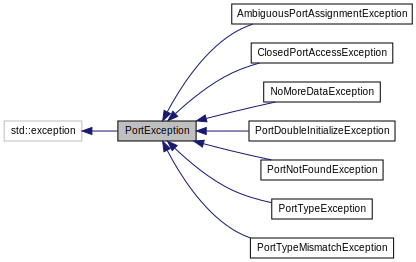
\includegraphics[width=350pt]{class_port_exception__inherit__graph}
\end{center}
\end{figure}


Collaboration diagram for Port\+Exception\+:
\nopagebreak
\begin{figure}[H]
\begin{center}
\leavevmode
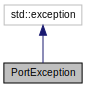
\includegraphics[width=158pt]{class_port_exception__coll__graph}
\end{center}
\end{figure}
\subsection*{Public Member Functions}
\begin{DoxyCompactItemize}
\item 
\hyperlink{class_port_exception_aec6ea14772ec4e06739ca2ae87115cbf}{Port\+Exception} (const std\+::string message)
\item 
\hypertarget{class_port_exception_adbdbaf084975880c9ba5d478c51a6273}{}\label{class_port_exception_adbdbaf084975880c9ba5d478c51a6273} 
virtual const char $\ast$ {\bfseries what} () const noexcept
\end{DoxyCompactItemize}


\subsection{Detailed Description}
\hyperlink{portexception_8hpp_source}{portexception.\+hpp} -\/ \begin{DoxyAuthor}{Author}
\+: Jonathan Beard 
\end{DoxyAuthor}
\begin{DoxyVersion}{Version}
\+: Wed Sep 3 14\+:52\+:27 2014
\end{DoxyVersion}
Copyright 2014 Jonathan Beard

Licensed under the Apache License, Version 2.\+0 (the \char`\"{}\+License\char`\"{}); you may not use this file except in compliance with the License. You may obtain a copy of the License at\+:

\href{http://www.apache.org/licenses/LICENSE-2.0}{\tt http\+://www.\+apache.\+org/licenses/\+L\+I\+C\+E\+N\+S\+E-\/2.\+0}

Unless required by applicable law or agreed to in writing, software distributed under the License is distributed on an \char`\"{}\+A\+S I\+S\char`\"{} B\+A\+S\+IS, W\+I\+T\+H\+O\+UT W\+A\+R\+R\+A\+N\+T\+I\+ES OR C\+O\+N\+D\+I\+T\+I\+O\+NS OF A\+NY K\+I\+ND, either express or implied. See the License for the specific language governing permissions and limitations under the License. 

Definition at line 24 of file portexception.\+hpp.



\subsection{Constructor \& Destructor Documentation}
\hypertarget{class_port_exception_aec6ea14772ec4e06739ca2ae87115cbf}{}\label{class_port_exception_aec6ea14772ec4e06739ca2ae87115cbf} 
\index{Port\+Exception@{Port\+Exception}!Port\+Exception@{Port\+Exception}}
\index{Port\+Exception@{Port\+Exception}!Port\+Exception@{Port\+Exception}}
\subsubsection{\texorpdfstring{Port\+Exception()}{PortException()}}
{\footnotesize\ttfamily Port\+Exception\+::\+Port\+Exception (\begin{DoxyParamCaption}\item[{const std\+::string}]{message }\end{DoxyParamCaption})}

\hyperlink{portexception_8cpp_source}{portexception.\+cpp} -\/ \begin{DoxyAuthor}{Author}
\+: Jonathan Beard 
\end{DoxyAuthor}
\begin{DoxyVersion}{Version}
\+: Wed Sep 3 14\+:52\+:27 2014
\end{DoxyVersion}
Copyright 2014 Jonathan Beard

Licensed under the Apache License, Version 2.\+0 (the \char`\"{}\+License\char`\"{}); you may not use this file except in compliance with the License. You may obtain a copy of the License at\+:

\href{http://www.apache.org/licenses/LICENSE-2.0}{\tt http\+://www.\+apache.\+org/licenses/\+L\+I\+C\+E\+N\+S\+E-\/2.\+0}

Unless required by applicable law or agreed to in writing, software distributed under the License is distributed on an \char`\"{}\+A\+S I\+S\char`\"{} B\+A\+S\+IS, W\+I\+T\+H\+O\+UT W\+A\+R\+R\+A\+N\+T\+I\+ES OR C\+O\+N\+D\+I\+T\+I\+O\+NS OF A\+NY K\+I\+ND, either express or implied. See the License for the specific language governing permissions and limitations under the License. 

Definition at line 22 of file portexception.\+cpp.


\begin{DoxyCode}
23 \{
24    (\textcolor{keyword}{this})->message = message;
25 \}
\end{DoxyCode}


The documentation for this class was generated from the following files\+:\begin{DoxyCompactItemize}
\item 
portexception.\+hpp\item 
portexception.\+cpp\end{DoxyCompactItemize}

\hypertarget{struct_port_info}{}\section{Port\+Info Struct Reference}
\label{struct_port_info}\index{Port\+Info@{Port\+Info}}


Collaboration diagram for Port\+Info\+:
\nopagebreak
\begin{figure}[H]
\begin{center}
\leavevmode
\includegraphics[width=350pt]{struct_port_info__coll__graph}
\end{center}
\end{figure}
\subsection*{Public Member Functions}
\begin{DoxyCompactItemize}
\item 
\hypertarget{struct_port_info_ada6f27ee68c0d489ad5a8ef41a990628}{}\label{struct_port_info_ada6f27ee68c0d489ad5a8ef41a990628} 
{\bfseries Port\+Info} (const std\+::type\+\_\+info \&the\+\_\+type)
\item 
\hypertarget{struct_port_info_a8a74d623dea1deab1d26920ece808dff}{}\label{struct_port_info_a8a74d623dea1deab1d26920ece808dff} 
{\bfseries Port\+Info} (const std\+::type\+\_\+info \&the\+\_\+type, void $\ast$const ptr, const std\+::size\+\_\+t nitems, const std\+::size\+\_\+t start\+\_\+index)
\item 
\hypertarget{struct_port_info_a8756457c158ca06d189b08b4b8fe3a12}{}\label{struct_port_info_a8756457c158ca06d189b08b4b8fe3a12} 
{\bfseries Port\+Info} (const \hyperlink{struct_port_info}{Port\+Info} \&other)
\item 
virtual \hyperlink{struct_port_info_a36e5aca1b7b20aace809490cebbc2d72}{$\sim$\+Port\+Info} ()
\item 
\hyperlink{class_f_i_f_o}{F\+I\+FO} $\ast$ \hyperlink{struct_port_info_a483d162fbe356e07381c6c5cfccb4f48}{get\+F\+I\+FO} ()
\item 
void \hyperlink{struct_port_info_a43a57cd624dcc44ccd9dcaba1d07a000}{set\+F\+I\+FO} (\hyperlink{class_f_i_f_o}{F\+I\+FO} $\ast$const in)
\end{DoxyCompactItemize}
\subsection*{Public Attributes}
\begin{DoxyCompactItemize}
\item 
\hypertarget{struct_port_info_af8148dcb4b8e6d355dbce4de10cc10cd}{}\label{struct_port_info_af8148dcb4b8e6d355dbce4de10cc10cd} 
\hyperlink{class_f_i_f_o}{F\+I\+FO} $\ast$ {\bfseries fifo\+\_\+a} = nullptr
\item 
\hypertarget{struct_port_info_a071d6f3662fd14dc6b3d12913eecd4ad}{}\label{struct_port_info_a071d6f3662fd14dc6b3d12913eecd4ad} 
\hyperlink{class_f_i_f_o}{F\+I\+FO} $\ast$ {\bfseries fifo\+\_\+b} = nullptr
\item 
std\+::type\+\_\+index \hyperlink{struct_port_info_a669818f0fde1da7b4a294c46e08d5980}{type}
\item 
std\+::map$<$ Type\+::\+Ring\+Buffer\+Type, instr\+\_\+map\+\_\+t $\ast$$>$ \hyperlink{struct_port_info_a714592b5ab1fa47b599903639b102a66}{const\+\_\+map}
\item 
split\+\_\+factory\+\_\+t \hyperlink{struct_port_info_a6b7e8758b84288a4378233251252be77}{split\+\_\+func} = nullptr
\item 
\hypertarget{struct_port_info_a79c530d0df178e81f8ced267162463ba}{}\label{struct_port_info_a79c530d0df178e81f8ced267162463ba} 
join\+\_\+factory\+\_\+t {\bfseries join\+\_\+func} = nullptr
\item 
\hypertarget{struct_port_info_a52680ae480484d347333615eb2100633}{}\label{struct_port_info_a52680ae480484d347333615eb2100633} 
\hyperlink{classraft_1_1kernel}{raft\+::kernel} $\ast$ {\bfseries my\+\_\+kernel} = nullptr
\item 
\hypertarget{struct_port_info_a52b0d512d88e2a2ca9efc2e6d3195526}{}\label{struct_port_info_a52b0d512d88e2a2ca9efc2e6d3195526} 
std\+::string {\bfseries my\+\_\+name} = \char`\"{}\char`\"{}
\item 
\hypertarget{struct_port_info_a68948477f69bccb9a273a02eaae782d4}{}\label{struct_port_info_a68948477f69bccb9a273a02eaae782d4} 
\hyperlink{classraft_1_1kernel}{raft\+::kernel} $\ast$ {\bfseries other\+\_\+kernel} = nullptr
\item 
\hypertarget{struct_port_info_a5a51ce33a630378cea7ef141efd41b95}{}\label{struct_port_info_a5a51ce33a630378cea7ef141efd41b95} 
std\+::string {\bfseries other\+\_\+name} = \char`\"{}\char`\"{}
\item 
bool \hyperlink{struct_port_info_a5da81ef07f28858445aa768700948cf2}{use\+\_\+my\+\_\+allocator} = false
\item 
\hypertarget{struct_port_info_ab63be643334befc42faef10a88af0f43}{}\label{struct_port_info_ab63be643334befc42faef10a88af0f43} 
bool {\bfseries out\+\_\+of\+\_\+order} = false
\item 
\hypertarget{struct_port_info_a8efd4554b05236d91b4d2025ce05ffda}{}\label{struct_port_info_a8efd4554b05236d91b4d2025ce05ffda} 
memory\+\_\+type {\bfseries mem} = heap
\item 
\hypertarget{struct_port_info_a18efecff2a108ef02f05e1ba140d8b07}{}\label{struct_port_info_a18efecff2a108ef02f05e1ba140d8b07} 
void $\ast$ {\bfseries existing\+\_\+buffer} = nullptr
\item 
\hypertarget{struct_port_info_a66ca647fbbb03cc60a7058c98407a26b}{}\label{struct_port_info_a66ca647fbbb03cc60a7058c98407a26b} 
std\+::size\+\_\+t {\bfseries nitems} = 0
\item 
\hypertarget{struct_port_info_aa21049cabf3bcc11580f05c247e7e5b0}{}\label{struct_port_info_aa21049cabf3bcc11580f05c247e7e5b0} 
std\+::size\+\_\+t {\bfseries start\+\_\+index} = 0
\item 
\hypertarget{struct_port_info_a3265b4628f68dc00a0c43f6fade694ca}{}\label{struct_port_info_a3265b4628f68dc00a0c43f6fade694ca} 
std\+::size\+\_\+t {\bfseries fixed\+\_\+buffer\+\_\+size} = 0
\end{DoxyCompactItemize}


\subsection{Detailed Description}


Definition at line 40 of file port\+\_\+info.\+hpp.



\subsection{Constructor \& Destructor Documentation}
\hypertarget{struct_port_info_a36e5aca1b7b20aace809490cebbc2d72}{}\label{struct_port_info_a36e5aca1b7b20aace809490cebbc2d72} 
\index{Port\+Info@{Port\+Info}!````~Port\+Info@{$\sim$\+Port\+Info}}
\index{````~Port\+Info@{$\sim$\+Port\+Info}!Port\+Info@{Port\+Info}}
\subsubsection{\texorpdfstring{$\sim$\+Port\+Info()}{~PortInfo()}}
{\footnotesize\ttfamily Port\+Info\+::$\sim$\+Port\+Info (\begin{DoxyParamCaption}{ }\end{DoxyParamCaption})\hspace{0.3cm}{\ttfamily [virtual]}}

alloc delete fifo object 

Definition at line 42 of file port\+\_\+info.\+cpp.


\begin{DoxyCode}
43 \{\textcolor{comment}{}
44 \textcolor{comment}{   /** alloc delete fifo object **/}
45 \}
\end{DoxyCode}


\subsection{Member Function Documentation}
\hypertarget{struct_port_info_a483d162fbe356e07381c6c5cfccb4f48}{}\label{struct_port_info_a483d162fbe356e07381c6c5cfccb4f48} 
\index{Port\+Info@{Port\+Info}!get\+F\+I\+FO@{get\+F\+I\+FO}}
\index{get\+F\+I\+FO@{get\+F\+I\+FO}!Port\+Info@{Port\+Info}}
\subsubsection{\texorpdfstring{get\+F\+I\+F\+O()}{getFIFO()}}
{\footnotesize\ttfamily \hyperlink{class_f_i_f_o}{F\+I\+FO} $\ast$ Port\+Info\+::get\+F\+I\+FO (\begin{DoxyParamCaption}{ }\end{DoxyParamCaption})}

get\+F\+I\+FO -\/ call this function to get a \hyperlink{class_f_i_f_o}{F\+I\+FO}, lock free but checks to make sure an update isn\textquotesingle{}t occuring. The ptr returned will be fine to use even if an update occurs while the ptr is in use since it won\textquotesingle{}t be deleted from the receiving end until the \hyperlink{class_f_i_f_o}{F\+I\+FO} is fully emptied. \begin{DoxyReturn}{Returns}
F\+I\+F\+O$\ast$ 
\end{DoxyReturn}
for most architectures that don\textquotesingle{}t need this, it\textquotesingle{}ll be optimized out after the first iteration 

Definition at line 49 of file port\+\_\+info.\+cpp.



Referenced by Allocate\+::initialize(), and dynalloc\+::run().


\begin{DoxyCode}
50 \{
51    \textcolor{keyword}{struct}\{
52       \hyperlink{class_f_i_f_o}{FIFO} *a;
53       \hyperlink{class_f_i_f_o}{FIFO} *b;
54    \}copy = \{ fifo\_a, fifo\_b \};\textcolor{comment}{}
55 \textcolor{comment}{   /** for most architectures that don't need this, it'll be optimized out after the first iteration **/}
56    \textcolor{keywordflow}{while}( copy.a != copy.b )
57    \{
58       copy.a = fifo\_a;
59       copy.b = fifo\_b;
60    \}
61    \textcolor{keywordflow}{return}( copy.a );
62 \}
\end{DoxyCode}
\hypertarget{struct_port_info_a43a57cd624dcc44ccd9dcaba1d07a000}{}\label{struct_port_info_a43a57cd624dcc44ccd9dcaba1d07a000} 
\index{Port\+Info@{Port\+Info}!set\+F\+I\+FO@{set\+F\+I\+FO}}
\index{set\+F\+I\+FO@{set\+F\+I\+FO}!Port\+Info@{Port\+Info}}
\subsubsection{\texorpdfstring{set\+F\+I\+F\+O()}{setFIFO()}}
{\footnotesize\ttfamily void Port\+Info\+::set\+F\+I\+FO (\begin{DoxyParamCaption}\item[{\hyperlink{class_f_i_f_o}{F\+I\+FO} $\ast$const}]{in }\end{DoxyParamCaption})}

set\+F\+I\+FO -\/ call this funciton to set a \hyperlink{class_f_i_f_o}{F\+I\+FO}, updates both pointers at the same time as opposed to doing it manually 
\begin{DoxyParams}{Parameters}
{\em in} & -\/ valid F\+I\+F\+O$\ast$, must not be nullptr \\
\hline
\end{DoxyParams}


Definition at line 65 of file port\+\_\+info.\+cpp.



Referenced by Allocate\+::initialize().


\begin{DoxyCode}
66 \{
67    assert( in != \textcolor{keyword}{nullptr} );
68    fifo\_a = in;
69    fifo\_b = in;
70 \}
\end{DoxyCode}


\subsection{Member Data Documentation}
\hypertarget{struct_port_info_a714592b5ab1fa47b599903639b102a66}{}\label{struct_port_info_a714592b5ab1fa47b599903639b102a66} 
\index{Port\+Info@{Port\+Info}!const\+\_\+map@{const\+\_\+map}}
\index{const\+\_\+map@{const\+\_\+map}!Port\+Info@{Port\+Info}}
\subsubsection{\texorpdfstring{const\+\_\+map}{const\_map}}
{\footnotesize\ttfamily std\+::map$<$ Type\+::\+Ring\+Buffer\+Type , instr\+\_\+map\+\_\+t$\ast$ $>$ Port\+Info\+::const\+\_\+map}

const\+\_\+map -\/ stores \char`\"{}builder\char`\"{} objects for each of the currenty implemented ring buffer types so that when the mapper is allocating ring buffers it may allocate one with the proper type. The first key is self explanatory for the most part, storing the ring buffer type. The second internal map key is \char`\"{}instrumented\char`\"{} vs. not. 

Definition at line 89 of file port\+\_\+info.\+hpp.



Referenced by Allocate\+::initialize(), Port\+::initialize\+Const\+Map(), and stdalloc\+::run().

\hypertarget{struct_port_info_a6b7e8758b84288a4378233251252be77}{}\label{struct_port_info_a6b7e8758b84288a4378233251252be77} 
\index{Port\+Info@{Port\+Info}!split\+\_\+func@{split\+\_\+func}}
\index{split\+\_\+func@{split\+\_\+func}!Port\+Info@{Port\+Info}}
\subsubsection{\texorpdfstring{split\+\_\+func}{split\_func}}
{\footnotesize\ttfamily split\+\_\+factory\+\_\+t Port\+Info\+::split\+\_\+func = nullptr}

N\+O\+TE\+: These are allocated by the run-\/time but not destroyed unless they\textquotesingle{}re used...they\textquotesingle{}ll of course be destroyed upon program termination. 

Definition at line 97 of file port\+\_\+info.\+hpp.



Referenced by raft\+::map\+::enable\+Duplication(), and Port\+::initialize\+Split().

\hypertarget{struct_port_info_a669818f0fde1da7b4a294c46e08d5980}{}\label{struct_port_info_a669818f0fde1da7b4a294c46e08d5980} 
\index{Port\+Info@{Port\+Info}!type@{type}}
\index{type@{type}!Port\+Info@{Port\+Info}}
\subsubsection{\texorpdfstring{type}{type}}
{\footnotesize\ttfamily std\+::type\+\_\+index Port\+Info\+::type}

the type of the port. regardless of if the buffer itself is impplemented or not. 

Definition at line 79 of file port\+\_\+info.\+hpp.



Referenced by Map\+Base\+::join(), and stdalloc\+::run().

\hypertarget{struct_port_info_a5da81ef07f28858445aa768700948cf2}{}\label{struct_port_info_a5da81ef07f28858445aa768700948cf2} 
\index{Port\+Info@{Port\+Info}!use\+\_\+my\+\_\+allocator@{use\+\_\+my\+\_\+allocator}}
\index{use\+\_\+my\+\_\+allocator@{use\+\_\+my\+\_\+allocator}!Port\+Info@{Port\+Info}}
\subsubsection{\texorpdfstring{use\+\_\+my\+\_\+allocator}{use\_my\_allocator}}
{\footnotesize\ttfamily bool Port\+Info\+::use\+\_\+my\+\_\+allocator = false}

runtime settings 

Definition at line 107 of file port\+\_\+info.\+hpp.



The documentation for this struct was generated from the following files\+:\begin{DoxyCompactItemize}
\item 
port\+\_\+info.\+hpp\item 
port\+\_\+info.\+cpp\end{DoxyCompactItemize}

\hypertarget{class_port_iterator}{}\section{Port\+Iterator Class Reference}
\label{class_port_iterator}\index{Port\+Iterator@{Port\+Iterator}}
Inheritance diagram for Port\+Iterator\+:\begin{figure}[H]
\begin{center}
\leavevmode
\includegraphics[height=2.000000cm]{class_port_iterator}
\end{center}
\end{figure}
\subsection*{Public Member Functions}
\begin{DoxyCompactItemize}
\item 
\hyperlink{class_port_iterator_a3d68fbe1ad98fbb8c7e25a9aecf8b5bf}{Port\+Iterator} (\hyperlink{structportmap__t}{portmap\+\_\+t} $\ast$const port\+\_\+map)
\item 
\hypertarget{class_port_iterator_acbaabd514cbbdcb0bb11e6ba381e9d3e}{}{\bfseries Port\+Iterator} (\hyperlink{structportmap__t}{portmap\+\_\+t} $\ast$const port\+\_\+map, const std\+::size\+\_\+t index)\label{class_port_iterator_acbaabd514cbbdcb0bb11e6ba381e9d3e}

\item 
\hypertarget{class_port_iterator_a68e10983b59c3889b73bff2635f2bb88}{}{\bfseries Port\+Iterator} (const \hyperlink{class_port_iterator}{Port\+Iterator} \&it)\label{class_port_iterator_a68e10983b59c3889b73bff2635f2bb88}

\item 
\hypertarget{class_port_iterator_a4695f037ef33e9ba809199401c9cb10f}{}\hyperlink{class_port_iterator}{Port\+Iterator} \& {\bfseries operator++} ()\label{class_port_iterator_a4695f037ef33e9ba809199401c9cb10f}

\item 
bool \hyperlink{class_port_iterator_ad41e4cf00699a49d6e0a30c8af3e7469}{operator==} (const \hyperlink{class_port_iterator}{Port\+Iterator} \&rhs)
\item 
\hypertarget{class_port_iterator_a4e2b7f7908ab1537205337d8d99a8e70}{}bool {\bfseries operator!=} (const \hyperlink{class_port_iterator}{Port\+Iterator} \&rhs)\label{class_port_iterator_a4e2b7f7908ab1537205337d8d99a8e70}

\item 
\hypertarget{class_port_iterator_a2d045feb7d7679a6968446fd78daed9d}{}F\+I\+F\+O \& {\bfseries operator$\ast$} ()\label{class_port_iterator_a2d045feb7d7679a6968446fd78daed9d}

\end{DoxyCompactItemize}


\subsection{Constructor \& Destructor Documentation}
\hypertarget{class_port_iterator_a3d68fbe1ad98fbb8c7e25a9aecf8b5bf}{}\index{Port\+Iterator@{Port\+Iterator}!Port\+Iterator@{Port\+Iterator}}
\index{Port\+Iterator@{Port\+Iterator}!Port\+Iterator@{Port\+Iterator}}
\subsubsection[{Port\+Iterator(portmap\+\_\+t $\ast$const port\+\_\+map)}]{\setlength{\rightskip}{0pt plus 5cm}Port\+Iterator\+::\+Port\+Iterator (
\begin{DoxyParamCaption}
\item[{{\bf portmap\+\_\+t} $\ast$const}]{port\+\_\+map}
\end{DoxyParamCaption}
)}\label{class_port_iterator_a3d68fbe1ad98fbb8c7e25a9aecf8b5bf}
portiterator.\+cpp -\/ \begin{DoxyAuthor}{Author}
\+: Jonathan Beard 
\end{DoxyAuthor}
\begin{DoxyVersion}{Version}
\+: Sun Oct 5 08\+:49\+:11 2014
\end{DoxyVersion}
Copyright 2014 Jonathan Beard

Licensed under the Apache License, Version 2.\+0 (the \char`\"{}\+License\char`\"{}); you may not use this file except in compliance with the License. You may obtain a copy of the License at\+:

\href{http://www.apache.org/licenses/LICENSE-2.0}{\tt http\+://www.\+apache.\+org/licenses/\+L\+I\+C\+E\+N\+S\+E-\/2.\+0}

Unless required by applicable law or agreed to in writing, software distributed under the License is distributed on an \char`\"{}\+A\+S I\+S\char`\"{} B\+A\+S\+I\+S, W\+I\+T\+H\+O\+U\+T W\+A\+R\+R\+A\+N\+T\+I\+E\+S O\+R C\+O\+N\+D\+I\+T\+I\+O\+N\+S O\+F A\+N\+Y K\+I\+N\+D, either express or implied. See the License for the specific language governing permissions and limitations under the License. 

\subsection{Member Function Documentation}
\hypertarget{class_port_iterator_ad41e4cf00699a49d6e0a30c8af3e7469}{}\index{Port\+Iterator@{Port\+Iterator}!operator==@{operator==}}
\index{operator==@{operator==}!Port\+Iterator@{Port\+Iterator}}
\subsubsection[{operator==(const Port\+Iterator \&rhs)}]{\setlength{\rightskip}{0pt plus 5cm}bool Port\+Iterator\+::operator== (
\begin{DoxyParamCaption}
\item[{const {\bf Port\+Iterator} \&}]{rhs}
\end{DoxyParamCaption}
)}\label{class_port_iterator_ad41e4cf00699a49d6e0a30c8af3e7469}
T\+O\+D\+O, on a more philosophical note, should this be a ptr comparison for the F\+I\+F\+O\textquotesingle{}s but then the end function would be harder to implement

The documentation for this class was generated from the following files\+:\begin{DoxyCompactItemize}
\item 
portiterator.\+hpp\item 
portiterator.\+cpp\end{DoxyCompactItemize}

\hypertarget{structportmap__t}{}\section{portmap\+\_\+t Struct Reference}
\label{structportmap__t}\index{portmap\+\_\+t@{portmap\+\_\+t}}


{\ttfamily \#include $<$portmap\+\_\+t.\+hpp$>$}

\subsection*{Public Attributes}
\begin{DoxyCompactItemize}
\item 
\hypertarget{structportmap__t_a898d883add7b8dc54ceef7e4ef27c94f}{}std\+::map$<$ std\+::string, \hyperlink{struct_port_info}{Port\+Info} $>$ {\bfseries map}\label{structportmap__t_a898d883add7b8dc54ceef7e4ef27c94f}

\item 
\hypertarget{structportmap__t_a4feb2a226aac9cd552668a8d4c8a3a7e}{}pthread\+\_\+mutex\+\_\+t {\bfseries mutex\+\_\+map}\label{structportmap__t_a4feb2a226aac9cd552668a8d4c8a3a7e}

\end{DoxyCompactItemize}


\subsection{Detailed Description}
\hyperlink{portmap__t_8hpp_source}{portmap\+\_\+t.\+hpp} -\/ \begin{DoxyAuthor}{Author}
\+: Jonathan Beard 
\end{DoxyAuthor}
\begin{DoxyVersion}{Version}
\+: Sun Oct 5 09\+:04\+:38 2014
\end{DoxyVersion}
Copyright 2014 Jonathan Beard

Licensed under the Apache License, Version 2.\+0 (the \char`\"{}\+License\char`\"{}); you may not use this file except in compliance with the License. You may obtain a copy of the License at\+:

\href{http://www.apache.org/licenses/LICENSE-2.0}{\tt http\+://www.\+apache.\+org/licenses/\+L\+I\+C\+E\+N\+S\+E-\/2.\+0}

Unless required by applicable law or agreed to in writing, software distributed under the License is distributed on an \char`\"{}\+A\+S I\+S\char`\"{} B\+A\+S\+I\+S, W\+I\+T\+H\+O\+U\+T W\+A\+R\+R\+A\+N\+T\+I\+E\+S O\+R C\+O\+N\+D\+I\+T\+I\+O\+N\+S O\+F A\+N\+Y K\+I\+N\+D, either express or implied. See the License for the specific language governing permissions and limitations under the License. 

The documentation for this struct was generated from the following files\+:\begin{DoxyCompactItemize}
\item 
portmap\+\_\+t.\+hpp\item 
portmap\+\_\+t.\+cpp\end{DoxyCompactItemize}

\hypertarget{class_port_not_found_exception}{}\section{Port\+Not\+Found\+Exception Class Reference}
\label{class_port_not_found_exception}\index{Port\+Not\+Found\+Exception@{Port\+Not\+Found\+Exception}}
Inheritance diagram for Port\+Not\+Found\+Exception\+:\begin{figure}[H]
\begin{center}
\leavevmode
\includegraphics[height=3.000000cm]{class_port_not_found_exception}
\end{center}
\end{figure}
\subsection*{Public Member Functions}
\begin{DoxyCompactItemize}
\item 
\hypertarget{class_port_not_found_exception_a2b233cfee5fc9eb16817e405107f95cd}{}{\bfseries Port\+Not\+Found\+Exception} (const std\+::string message)\label{class_port_not_found_exception_a2b233cfee5fc9eb16817e405107f95cd}

\end{DoxyCompactItemize}


The documentation for this class was generated from the following files\+:\begin{DoxyCompactItemize}
\item 
portexception.\+hpp\item 
portexception.\+cpp\end{DoxyCompactItemize}

\hypertarget{class_port_template}{}\section{Port\+Template Class Reference}
\label{class_port_template}\index{Port\+Template@{Port\+Template}}


{\ttfamily \#include $<$porttemplate.\+hpp$>$}

\subsection*{Protected Attributes}
\begin{DoxyCompactItemize}
\item 
\hypertarget{class_port_template_a1930a44af30c62b60b04e22bf83cbc34}{}std\+::map$<$ std\+::string, \hyperlink{struct_port_info}{Port\+Info} \& $>$ {\bfseries map}\label{class_port_template_a1930a44af30c62b60b04e22bf83cbc34}

\end{DoxyCompactItemize}


\subsection{Detailed Description}
\hyperlink{porttemplate_8hpp_source}{porttemplate.\+hpp} -\/ This object is designed to be used in conjunction with a Sub\+Map object, essentially its just a container to hold reference to the input and output ports to this sub-\/map so that the library doesn\textquotesingle{}t have to search the entire map when the Sub\+Map object is added to the main map.

\begin{DoxyAuthor}{Author}
\+: Jonathan Beard 
\end{DoxyAuthor}
\begin{DoxyVersion}{Version}
\+: Sun Nov 30 10\+:09\+:25 2014
\end{DoxyVersion}
Copyright 2014 Jonathan Beard

Licensed under the Apache License, Version 2.\+0 (the \char`\"{}\+License\char`\"{}); you may not use this file except in compliance with the License. You may obtain a copy of the License at\+:

\href{http://www.apache.org/licenses/LICENSE-2.0}{\tt http\+://www.\+apache.\+org/licenses/\+L\+I\+C\+E\+N\+S\+E-\/2.\+0}

Unless required by applicable law or agreed to in writing, software distributed under the License is distributed on an \char`\"{}\+A\+S I\+S\char`\"{} B\+A\+S\+I\+S, W\+I\+T\+H\+O\+U\+T W\+A\+R\+R\+A\+N\+T\+I\+E\+S O\+R C\+O\+N\+D\+I\+T\+I\+O\+N\+S O\+F A\+N\+Y K\+I\+N\+D, either express or implied. See the License for the specific language governing permissions and limitations under the License. 

The documentation for this class was generated from the following file\+:\begin{DoxyCompactItemize}
\item 
porttemplate.\+hpp\end{DoxyCompactItemize}

\hypertarget{class_port_type_exception}{}\section{Port\+Type\+Exception Class Reference}
\label{class_port_type_exception}\index{Port\+Type\+Exception@{Port\+Type\+Exception}}
Inheritance diagram for Port\+Type\+Exception\+:\begin{figure}[H]
\begin{center}
\leavevmode
\includegraphics[height=3.000000cm]{class_port_type_exception}
\end{center}
\end{figure}
\subsection*{Public Member Functions}
\begin{DoxyCompactItemize}
\item 
\hypertarget{class_port_type_exception_aa3154797084de9cfe74b653bf3e63ee2}{}{\bfseries Port\+Type\+Exception} (const std\+::string message)\label{class_port_type_exception_aa3154797084de9cfe74b653bf3e63ee2}

\end{DoxyCompactItemize}


The documentation for this class was generated from the following files\+:\begin{DoxyCompactItemize}
\item 
portexception.\+hpp\item 
portexception.\+cpp\end{DoxyCompactItemize}

\hypertarget{class_port_type_mismatch_exception}{}\section{Port\+Type\+Mismatch\+Exception Class Reference}
\label{class_port_type_mismatch_exception}\index{Port\+Type\+Mismatch\+Exception@{Port\+Type\+Mismatch\+Exception}}
Inheritance diagram for Port\+Type\+Mismatch\+Exception\+:\begin{figure}[H]
\begin{center}
\leavevmode
\includegraphics[height=3.000000cm]{class_port_type_mismatch_exception}
\end{center}
\end{figure}
\subsection*{Public Member Functions}
\begin{DoxyCompactItemize}
\item 
\hypertarget{class_port_type_mismatch_exception_aa4fa596cc94ecf73220fb1baeba44247}{}{\bfseries Port\+Type\+Mismatch\+Exception} (const std\+::string message)\label{class_port_type_mismatch_exception_aa4fa596cc94ecf73220fb1baeba44247}

\end{DoxyCompactItemize}


The documentation for this class was generated from the following files\+:\begin{DoxyCompactItemize}
\item 
portexception.\+hpp\item 
portexception.\+cpp\end{DoxyCompactItemize}

\hypertarget{classroundrobin}{}\section{roundrobin Class Reference}
\label{classroundrobin}\index{roundrobin@{roundrobin}}


{\ttfamily \#include $<$roundrobin.\+hpp$>$}

Inheritance diagram for roundrobin\+:\begin{figure}[H]
\begin{center}
\leavevmode
\includegraphics[height=2.000000cm]{classroundrobin}
\end{center}
\end{figure}
\subsection*{Protected Member Functions}
\begin{DoxyCompactItemize}
\item 
virtual F\+I\+F\+O $\ast$ \hyperlink{classroundrobin_acd670a96e62905062e50b21c3d5d64c5}{select\+\_\+fifo} (\hyperlink{class_port}{Port} \&port\+\_\+list, const functype type)
\end{DoxyCompactItemize}
\subsection*{Additional Inherited Members}


\subsection{Detailed Description}
\hyperlink{roundrobin_8hpp_source}{roundrobin.\+hpp} -\/ \begin{DoxyAuthor}{Author}
\+: Jonathan Beard 
\end{DoxyAuthor}
\begin{DoxyVersion}{Version}
\+: Tue Oct 28 13\+:05\+:38 2014
\end{DoxyVersion}
Copyright 2014 Jonathan Beard

Licensed under the Apache License, Version 2.\+0 (the \char`\"{}\+License\char`\"{}); you may not use this file except in compliance with the License. You may obtain a copy of the License at\+:

\href{http://www.apache.org/licenses/LICENSE-2.0}{\tt http\+://www.\+apache.\+org/licenses/\+L\+I\+C\+E\+N\+S\+E-\/2.\+0}

Unless required by applicable law or agreed to in writing, software distributed under the License is distributed on an \char`\"{}\+A\+S I\+S\char`\"{} B\+A\+S\+I\+S, W\+I\+T\+H\+O\+U\+T W\+A\+R\+R\+A\+N\+T\+I\+E\+S O\+R C\+O\+N\+D\+I\+T\+I\+O\+N\+S O\+F A\+N\+Y K\+I\+N\+D, either express or implied. See the License for the specific language governing permissions and limitations under the License. 

\subsection{Member Function Documentation}
\hypertarget{classroundrobin_acd670a96e62905062e50b21c3d5d64c5}{}\index{roundrobin@{roundrobin}!select\+\_\+fifo@{select\+\_\+fifo}}
\index{select\+\_\+fifo@{select\+\_\+fifo}!roundrobin@{roundrobin}}
\subsubsection[{select\+\_\+fifo(\+Port \&port\+\_\+list, const functype type)}]{\setlength{\rightskip}{0pt plus 5cm}F\+I\+F\+O $\ast$ roundrobin\+::select\+\_\+fifo (
\begin{DoxyParamCaption}
\item[{{\bf Port} \&}]{port\+\_\+list, }
\item[{const functype}]{type}
\end{DoxyParamCaption}
)\hspace{0.3cm}{\ttfamily [protected]}, {\ttfamily [virtual]}}\label{classroundrobin_acd670a96e62905062e50b21c3d5d64c5}
T\+O\+D\+O, big assumption here is that eventually a port will have space

Implements \hyperlink{classsplitmethod}{splitmethod}.



The documentation for this class was generated from the following files\+:\begin{DoxyCompactItemize}
\item 
roundrobin.\+hpp\item 
roundrobin.\+cpp\end{DoxyCompactItemize}

\hypertarget{structsched__cmd__t}{}\section{sched\+\_\+cmd\+\_\+t Struct Reference}
\label{structsched__cmd__t}\index{sched\+\_\+cmd\+\_\+t@{sched\+\_\+cmd\+\_\+t}}
\subsection*{Public Member Functions}
\begin{DoxyCompactItemize}
\item 
\hypertarget{structsched__cmd__t_a812b771fa21587d7b9888226e9ae0ce3}{}{\bfseries sched\+\_\+cmd\+\_\+t} (const schedule\+::sched\+\_\+cmd \hyperlink{structsched__cmd__t_ab4ecf8a7b468db75074c0ba1493caac7}{cmd}, \hyperlink{classraft_1_1kernel}{raft\+::kernel} $\ast$\hyperlink{structsched__cmd__t_a8f78af789430b7661f52de7365abcdbc}{kernel})\label{structsched__cmd__t_a812b771fa21587d7b9888226e9ae0ce3}

\item 
\hypertarget{structsched__cmd__t_a3a54e714aeba16cfe2faa5f2b082c8b8}{}{\bfseries sched\+\_\+cmd\+\_\+t} (const \hyperlink{structsched__cmd__t}{sched\+\_\+cmd\+\_\+t} \&other)\label{structsched__cmd__t_a3a54e714aeba16cfe2faa5f2b082c8b8}

\end{DoxyCompactItemize}
\subsection*{Public Attributes}
\begin{DoxyCompactItemize}
\item 
schedule\+::sched\+\_\+cmd \hyperlink{structsched__cmd__t_ab4ecf8a7b468db75074c0ba1493caac7}{cmd} = schedule\+::add
\item 
\hyperlink{classraft_1_1kernel}{raft\+::kernel} $\ast$ \hyperlink{structsched__cmd__t_a8f78af789430b7661f52de7365abcdbc}{kernel} = nullptr
\end{DoxyCompactItemize}


\subsection{Member Data Documentation}
\hypertarget{structsched__cmd__t_ab4ecf8a7b468db75074c0ba1493caac7}{}\index{sched\+\_\+cmd\+\_\+t@{sched\+\_\+cmd\+\_\+t}!cmd@{cmd}}
\index{cmd@{cmd}!sched\+\_\+cmd\+\_\+t@{sched\+\_\+cmd\+\_\+t}}
\subsubsection[{cmd}]{\setlength{\rightskip}{0pt plus 5cm}schedule\+::sched\+\_\+cmd sched\+\_\+cmd\+\_\+t\+::cmd = schedule\+::add}\label{structsched__cmd__t_ab4ecf8a7b468db75074c0ba1493caac7}
some reasonable default \hypertarget{structsched__cmd__t_a8f78af789430b7661f52de7365abcdbc}{}\index{sched\+\_\+cmd\+\_\+t@{sched\+\_\+cmd\+\_\+t}!kernel@{kernel}}
\index{kernel@{kernel}!sched\+\_\+cmd\+\_\+t@{sched\+\_\+cmd\+\_\+t}}
\subsubsection[{kernel}]{\setlength{\rightskip}{0pt plus 5cm}{\bf raft\+::kernel}$\ast$ sched\+\_\+cmd\+\_\+t\+::kernel = nullptr}\label{structsched__cmd__t_a8f78af789430b7661f52de7365abcdbc}
default == null 

The documentation for this struct was generated from the following file\+:\begin{DoxyCompactItemize}
\item 
sched\+\_\+cmd\+\_\+t.\+hpp\end{DoxyCompactItemize}

\hypertarget{class_schedule}{}\section{Schedule Class Reference}
\label{class_schedule}\index{Schedule@{Schedule}}
Inheritance diagram for Schedule\+:\begin{figure}[H]
\begin{center}
\leavevmode
\includegraphics[height=2.000000cm]{class_schedule}
\end{center}
\end{figure}
\subsection*{Public Member Functions}
\begin{DoxyCompactItemize}
\item 
\hyperlink{class_schedule_ad88c01f0ebf0c2f3bfa3ca2fe7ca3e8f}{Schedule} (\hyperlink{class_map}{Map} \&map)
\item 
virtual \hyperlink{class_schedule_a4806b985197d35c00b9e707c0ed87998}{$\sim$\+Schedule} ()
\item 
virtual void \hyperlink{class_schedule_ab6ad5540ecdef6b472b4e8242a47c4ee}{start} ()=0
\item 
virtual void \hyperlink{class_schedule_a5180032a0c2135507859ccf2a4eea1ab}{init} ()
\item 
void \hyperlink{class_schedule_a6a722f6e76c8b8dc67874d9974b6d641}{schedule\+Kernel} (\hyperlink{classraft_1_1kernel}{raft\+::kernel} $\ast$const kernel)
\end{DoxyCompactItemize}
\subsection*{Static Public Member Functions}
\begin{DoxyCompactItemize}
\item 
static bool \hyperlink{class_schedule_acf28b4a4231e693585751a035873615c}{kernel\+Run} (\hyperlink{classraft_1_1kernel}{raft\+::kernel} $\ast$const kernel, volatile bool \&finished, jmp\+\_\+buf $\ast$gotostate=nullptr, jmp\+\_\+buf $\ast$kernel\+\_\+state=nullptr)
\end{DoxyCompactItemize}
\subsection*{Protected Member Functions}
\begin{DoxyCompactItemize}
\item 
\hypertarget{class_schedule_addff3f2e72caab274963cc888faa2f6b}{}virtual void {\bfseries handle\+Schedule} (\hyperlink{classraft_1_1kernel}{raft\+::kernel} $\ast$const kernel)=0\label{class_schedule_addff3f2e72caab274963cc888faa2f6b}

\end{DoxyCompactItemize}
\subsection*{Static Protected Member Functions}
\begin{DoxyCompactItemize}
\item 
static raft\+::kstatus \hyperlink{class_schedule_a85de3d48407aa378ccc86a4a4206b32a}{check\+System\+Signal} (\hyperlink{classraft_1_1kernel}{raft\+::kernel} $\ast$const kernel, void $\ast$data, \hyperlink{class_system_signal_handler}{System\+Signal\+Handler} \&\hyperlink{class_schedule_ad248e99611a87776fb411836cd46a603}{handlers})
\item 
static raft\+::kstatus \hyperlink{class_schedule_a5167d622689a34ea5f3a065304295521}{quit\+Handler} (F\+I\+F\+O \&fifo, \hyperlink{classraft_1_1kernel}{raft\+::kernel} $\ast$kernel, const raft\+::signal signal, void $\ast$data)
\item 
\hypertarget{class_schedule_a3bf10fd9419c58849d7be98336dc0aff}{}static void {\bfseries invalidate\+Output\+Ports} (\hyperlink{classraft_1_1kernel}{raft\+::kernel} $\ast$kernel)\label{class_schedule_a3bf10fd9419c58849d7be98336dc0aff}

\item 
static bool \hyperlink{class_schedule_ac23de3dd63554401fd0d8d23b60eecfa}{kernel\+Has\+Input\+Data} (\hyperlink{classraft_1_1kernel}{raft\+::kernel} $\ast$kernel)
\item 
static bool \hyperlink{class_schedule_a2e2035e0c0666054f8401ad2b3792854}{kernel\+Has\+No\+Input\+Ports} (\hyperlink{classraft_1_1kernel}{raft\+::kernel} $\ast$kernel)
\end{DoxyCompactItemize}
\subsection*{Protected Attributes}
\begin{DoxyCompactItemize}
\item 
\hyperlink{class_system_signal_handler}{System\+Signal\+Handler} \hyperlink{class_schedule_ad248e99611a87776fb411836cd46a603}{handlers}
\item 
kernelkeeper \& \hyperlink{class_schedule_a1a448b0d48e656f94db65a70cedd8eed}{kernel\+\_\+set}
\item 
\hypertarget{class_schedule_ad4c895eb77d8287a9a19215cced7af7b}{}kernelkeeper \& {\bfseries source\+\_\+kernels}\label{class_schedule_ad4c895eb77d8287a9a19215cced7af7b}

\item 
\hypertarget{class_schedule_aebf2c26334eae760032d82a016898043}{}kernelkeeper \& {\bfseries dst\+\_\+kernels}\label{class_schedule_aebf2c26334eae760032d82a016898043}

\end{DoxyCompactItemize}


\subsection{Constructor \& Destructor Documentation}
\hypertarget{class_schedule_ad88c01f0ebf0c2f3bfa3ca2fe7ca3e8f}{}\index{Schedule@{Schedule}!Schedule@{Schedule}}
\index{Schedule@{Schedule}!Schedule@{Schedule}}
\subsubsection[{Schedule(\+Map \&map)}]{\setlength{\rightskip}{0pt plus 5cm}Schedule\+::\+Schedule (
\begin{DoxyParamCaption}
\item[{{\bf Map} \&}]{map}
\end{DoxyParamCaption}
)}\label{class_schedule_ad88c01f0ebf0c2f3bfa3ca2fe7ca3e8f}
\hyperlink{class_schedule}{Schedule} -\/ base constructor takes a map object so that all sub-\/classes can access some of the map features through the schedule sub-\/class accessors. 
\begin{DoxyParams}{Parameters}
{\em map} & -\/ \hyperlink{class_map}{Map}\& \\
\hline
\end{DoxyParams}
\hypertarget{class_schedule_a4806b985197d35c00b9e707c0ed87998}{}\index{Schedule@{Schedule}!````~Schedule@{$\sim$\+Schedule}}
\index{````~Schedule@{$\sim$\+Schedule}!Schedule@{Schedule}}
\subsubsection[{$\sim$\+Schedule()}]{\setlength{\rightskip}{0pt plus 5cm}Schedule\+::$\sim$\+Schedule (
\begin{DoxyParamCaption}
{}
\end{DoxyParamCaption}
)\hspace{0.3cm}{\ttfamily [virtual]}}\label{class_schedule_a4806b985197d35c00b9e707c0ed87998}
destructor, takes care of cleanup nothing to do at the moment 

\subsection{Member Function Documentation}
\hypertarget{class_schedule_a85de3d48407aa378ccc86a4a4206b32a}{}\index{Schedule@{Schedule}!check\+System\+Signal@{check\+System\+Signal}}
\index{check\+System\+Signal@{check\+System\+Signal}!Schedule@{Schedule}}
\subsubsection[{check\+System\+Signal(raft\+::kernel $\ast$const kernel, void $\ast$data, System\+Signal\+Handler \&handlers)}]{\setlength{\rightskip}{0pt plus 5cm}raft\+::kstatus Schedule\+::check\+System\+Signal (
\begin{DoxyParamCaption}
\item[{{\bf raft\+::kernel} $\ast$const}]{kernel, }
\item[{void $\ast$}]{data, }
\item[{{\bf System\+Signal\+Handler} \&}]{handlers}
\end{DoxyParamCaption}
)\hspace{0.3cm}{\ttfamily [static]}, {\ttfamily [protected]}}\label{class_schedule_a85de3d48407aa378ccc86a4a4206b32a}
check\+System\+Signal -\/ check the incomming streams for the param kernel for any system signals, if there is one then consume the signal and perform the appropriate action. 
\begin{DoxyParams}{Parameters}
{\em kernel} & -\/ \hyperlink{classraft_1_1kernel}{raft\+::kernel} \\
\hline
{\em data} & -\/ void$\ast$, use this if any further info is needed in future implementations of handlers \\
\hline
\end{DoxyParams}
\begin{DoxyReturn}{Returns}
raft\+::kstatus, proceed unless a stop signal is received 
\end{DoxyReturn}
T\+O\+D\+O, right now there is special behavior for term signal only, what should we do with others? Need to decide that.\hypertarget{class_schedule_a5180032a0c2135507859ccf2a4eea1ab}{}\index{Schedule@{Schedule}!init@{init}}
\index{init@{init}!Schedule@{Schedule}}
\subsubsection[{init()}]{\setlength{\rightskip}{0pt plus 5cm}void Schedule\+::init (
\begin{DoxyParamCaption}
{}
\end{DoxyParamCaption}
)\hspace{0.3cm}{\ttfamily [virtual]}}\label{class_schedule_a5180032a0c2135507859ccf2a4eea1ab}
init -\/ call to pre-\/process all kernels, this function is called by the map object befure calling start. default, do nothing \hypertarget{class_schedule_ac23de3dd63554401fd0d8d23b60eecfa}{}\index{Schedule@{Schedule}!kernel\+Has\+Input\+Data@{kernel\+Has\+Input\+Data}}
\index{kernel\+Has\+Input\+Data@{kernel\+Has\+Input\+Data}!Schedule@{Schedule}}
\subsubsection[{kernel\+Has\+Input\+Data(raft\+::kernel $\ast$kernel)}]{\setlength{\rightskip}{0pt plus 5cm}bool Schedule\+::kernel\+Has\+Input\+Data (
\begin{DoxyParamCaption}
\item[{{\bf raft\+::kernel} $\ast$}]{kernel}
\end{DoxyParamCaption}
)\hspace{0.3cm}{\ttfamily [static]}, {\ttfamily [protected]}}\label{class_schedule_ac23de3dd63554401fd0d8d23b60eecfa}
kernel\+Has\+Input\+Data -\/ check each input port for available data, returns true if any of the input ports has available data. 
\begin{DoxyParams}{Parameters}
{\em kernel} & -\/ \hyperlink{classraft_1_1kernel}{raft\+::kernel} \\
\hline
\end{DoxyParams}
\begin{DoxyReturn}{Returns}
bool -\/ true if input data available. 
\end{DoxyReturn}
only output ports, keep calling till exits \hypertarget{class_schedule_a2e2035e0c0666054f8401ad2b3792854}{}\index{Schedule@{Schedule}!kernel\+Has\+No\+Input\+Ports@{kernel\+Has\+No\+Input\+Ports}}
\index{kernel\+Has\+No\+Input\+Ports@{kernel\+Has\+No\+Input\+Ports}!Schedule@{Schedule}}
\subsubsection[{kernel\+Has\+No\+Input\+Ports(raft\+::kernel $\ast$kernel)}]{\setlength{\rightskip}{0pt plus 5cm}bool Schedule\+::kernel\+Has\+No\+Input\+Ports (
\begin{DoxyParamCaption}
\item[{{\bf raft\+::kernel} $\ast$}]{kernel}
\end{DoxyParamCaption}
)\hspace{0.3cm}{\ttfamily [static]}, {\ttfamily [protected]}}\label{class_schedule_a2e2035e0c0666054f8401ad2b3792854}
kernel\+Has\+No\+Input\+Ports -\/ pretty much exactly like the function name says, if the param kernel has no valid input ports (this function assumes that \hyperlink{class_schedule_ac23de3dd63554401fd0d8d23b60eecfa}{kernel\+Has\+Input\+Data()} has been called and returns false before this function is called) then it returns true.  kernel -\/ \hyperlink{classraft_1_1kernel}{raft\+::kernel}$\ast$ \begin{DoxyReturn}{Returns}
bool -\/ true if no valid input ports avail 
\end{DoxyReturn}
assume data check is already complete \hypertarget{class_schedule_acf28b4a4231e693585751a035873615c}{}\index{Schedule@{Schedule}!kernel\+Run@{kernel\+Run}}
\index{kernel\+Run@{kernel\+Run}!Schedule@{Schedule}}
\subsubsection[{kernel\+Run(raft\+::kernel $\ast$const kernel, volatile bool \&finished, jmp\+\_\+buf $\ast$gotostate=nullptr, jmp\+\_\+buf $\ast$kernel\+\_\+state=nullptr)}]{\setlength{\rightskip}{0pt plus 5cm}bool Schedule\+::kernel\+Run (
\begin{DoxyParamCaption}
\item[{{\bf raft\+::kernel} $\ast$const}]{kernel, }
\item[{volatile bool \&}]{finished, }
\item[{jmp\+\_\+buf $\ast$}]{gotostate = {\ttfamily nullptr}, }
\item[{jmp\+\_\+buf $\ast$}]{kernel\+\_\+state = {\ttfamily nullptr}}
\end{DoxyParamCaption}
)\hspace{0.3cm}{\ttfamily [static]}}\label{class_schedule_acf28b4a4231e693585751a035873615c}
kernel\+Run -\/ all the logic necessary to run a single kernel successfully. Any additional signal handling should be handled by this function as its the only one that will be universally called by the scheduler. 
\begin{DoxyParams}{Parameters}
{\em kernel} & -\/ \hyperlink{classraft_1_1kernel}{raft\+::kernel} $\ast$const object, non-\/null kernel \\
\hline
{\em finished} & -\/ volatile bool -\/ function sets to true when done. \\
\hline
\end{DoxyParams}
\begin{DoxyReturn}{Returns}
true if run with no need for jmp\+\_\+buf, false if the scheduler needs to run again with the kernel\+\_\+state 
\end{DoxyReturn}
must recheck data items again after port valid check, there could have been a push between these two conditional statements.\hypertarget{class_schedule_a5167d622689a34ea5f3a065304295521}{}\index{Schedule@{Schedule}!quit\+Handler@{quit\+Handler}}
\index{quit\+Handler@{quit\+Handler}!Schedule@{Schedule}}
\subsubsection[{quit\+Handler(\+F\+I\+F\+O \&fifo, raft\+::kernel $\ast$kernel, const raft\+::signal signal, void $\ast$data)}]{\setlength{\rightskip}{0pt plus 5cm}raft\+::kstatus Schedule\+::quit\+Handler (
\begin{DoxyParamCaption}
\item[{F\+I\+F\+O \&}]{fifo, }
\item[{{\bf raft\+::kernel} $\ast$}]{kernel, }
\item[{const raft\+::signal}]{signal, }
\item[{void $\ast$}]{data}
\end{DoxyParamCaption}
)\hspace{0.3cm}{\ttfamily [static]}, {\ttfamily [protected]}}\label{class_schedule_a5167d622689a34ea5f3a065304295521}
quite\+Handler -\/ performs the actions needed when a port sends a quite signal (normal termination), this is most likely due to the end of data. 
\begin{DoxyParams}{Parameters}
{\em fifo} & -\/ F\+I\+F\+O\& that sent the signal \\
\hline
{\em kernel} & -\/ \hyperlink{classraft_1_1kernel}{raft\+::kernel}$\ast$ \\
\hline
{\em signal} & -\/ raft\+::signal \\
\hline
{\em data} & -\/ void$\ast$, vain attempt to future proof \\
\hline
\end{DoxyParams}
N\+O\+T\+E\+: This should be the only action needed currently, however that may change in the futre with more features and systems added.\hypertarget{class_schedule_a6a722f6e76c8b8dc67874d9974b6d641}{}\index{Schedule@{Schedule}!schedule\+Kernel@{schedule\+Kernel}}
\index{schedule\+Kernel@{schedule\+Kernel}!Schedule@{Schedule}}
\subsubsection[{schedule\+Kernel(raft\+::kernel $\ast$const kernel)}]{\setlength{\rightskip}{0pt plus 5cm}void Schedule\+::schedule\+Kernel (
\begin{DoxyParamCaption}
\item[{{\bf raft\+::kernel} $\ast$const}]{kernel}
\end{DoxyParamCaption}
)}\label{class_schedule_a6a722f6e76c8b8dc67874d9974b6d641}
schedule\+Kernel -\/ adds the kernel \char`\"{}kernel\char`\"{} to the schedule, ensures that it is run. Other than that there are no guarantees for its execution. It is purely virtual in its implementation. Before you drop in a kernel, it better be ready to go..all allocations should be complete. 
\begin{DoxyParams}{Parameters}
{\em kernel} & -\/ \hyperlink{classraft_1_1kernel}{raft\+::kernel}$\ast$ \\
\hline
\end{DoxyParams}
N\+O\+T\+E\+: The kernel param should be ready to rock, we just need to add it here. The data structures xx\+\_\+kernels all expect a fully ready kernel, well the threads monitoring the system do at least and this is one. What we need to do to kick off the execution is add it to the handle\+Schedule virtual function which is implemented by each scheduler.\hypertarget{class_schedule_ab6ad5540ecdef6b472b4e8242a47c4ee}{}\index{Schedule@{Schedule}!start@{start}}
\index{start@{start}!Schedule@{Schedule}}
\subsubsection[{start()=0}]{\setlength{\rightskip}{0pt plus 5cm}virtual void Schedule\+::start (
\begin{DoxyParamCaption}
{}
\end{DoxyParamCaption}
)\hspace{0.3cm}{\ttfamily [pure virtual]}}\label{class_schedule_ab6ad5540ecdef6b472b4e8242a47c4ee}
start -\/ called to start execution of all kernels. Implementation specific so it is purely virtual. 

Implemented in \hyperlink{classpool__schedule_ab67558a44404e42ba032f799c0f424a7}{pool\+\_\+schedule}, and \hyperlink{classsimple__schedule_ad60a7608111e011d0c04f6ac566cfd8c}{simple\+\_\+schedule}.



\subsection{Member Data Documentation}
\hypertarget{class_schedule_ad248e99611a87776fb411836cd46a603}{}\index{Schedule@{Schedule}!handlers@{handlers}}
\index{handlers@{handlers}!Schedule@{Schedule}}
\subsubsection[{handlers}]{\setlength{\rightskip}{0pt plus 5cm}{\bf System\+Signal\+Handler} Schedule\+::handlers\hspace{0.3cm}{\ttfamily [protected]}}\label{class_schedule_ad248e99611a87776fb411836cd46a603}
signal handlers \hypertarget{class_schedule_a1a448b0d48e656f94db65a70cedd8eed}{}\index{Schedule@{Schedule}!kernel\+\_\+set@{kernel\+\_\+set}}
\index{kernel\+\_\+set@{kernel\+\_\+set}!Schedule@{Schedule}}
\subsubsection[{kernel\+\_\+set}]{\setlength{\rightskip}{0pt plus 5cm}kernelkeeper\& Schedule\+::kernel\+\_\+set\hspace{0.3cm}{\ttfamily [protected]}}\label{class_schedule_a1a448b0d48e656f94db65a70cedd8eed}
kernel set 

The documentation for this class was generated from the following files\+:\begin{DoxyCompactItemize}
\item 
schedule.\+hpp\item 
schedule.\+cpp\end{DoxyCompactItemize}

\hypertarget{classsimple__schedule}{}\section{simple\+\_\+schedule Class Reference}
\label{classsimple__schedule}\index{simple\+\_\+schedule@{simple\+\_\+schedule}}
Inheritance diagram for simple\+\_\+schedule\+:\begin{figure}[H]
\begin{center}
\leavevmode
\includegraphics[height=2.000000cm]{classsimple__schedule}
\end{center}
\end{figure}
\subsection*{Classes}
\begin{DoxyCompactItemize}
\item 
struct \hyperlink{structsimple__schedule_1_1thread__data}{thread\+\_\+data}
\item 
struct \hyperlink{structsimple__schedule_1_1thread__info__t}{thread\+\_\+info\+\_\+t}
\end{DoxyCompactItemize}
\subsection*{Public Member Functions}
\begin{DoxyCompactItemize}
\item 
\hyperlink{classsimple__schedule_a25bafe4199780c7abda6a9df3a599d88}{simple\+\_\+schedule} (\hyperlink{class_map}{Map} \&map)
\item 
virtual void \hyperlink{classsimple__schedule_ad60a7608111e011d0c04f6ac566cfd8c}{start} ()
\end{DoxyCompactItemize}
\subsection*{Protected Member Functions}
\begin{DoxyCompactItemize}
\item 
void \hyperlink{classsimple__schedule_aafebb0cc13b4539387790ff54ea40830}{handle\+Schedule} (\hyperlink{classraft_1_1kernel}{raft\+::kernel} $\ast$const kernel)
\end{DoxyCompactItemize}
\subsection*{Static Protected Member Functions}
\begin{DoxyCompactItemize}
\item 
\hypertarget{classsimple__schedule_a4fac873aedbc372a9a008cf02b30c048}{}static void $\ast$ {\bfseries simple\+\_\+run} (void $\ast$data)\label{classsimple__schedule_a4fac873aedbc372a9a008cf02b30c048}

\end{DoxyCompactItemize}
\subsection*{Protected Attributes}
\begin{DoxyCompactItemize}
\item 
\hypertarget{classsimple__schedule_afb23a2c4ff29959b3f43d5802ac76c79}{}pthread\+\_\+mutex\+\_\+t {\bfseries thread\+\_\+map\+\_\+mutex}\label{classsimple__schedule_afb23a2c4ff29959b3f43d5802ac76c79}

\item 
\hypertarget{classsimple__schedule_a1c6f1b93365dc324a72c467765ffef86}{}std\+::vector$<$ \hyperlink{structsimple__schedule_1_1thread__info__t}{thread\+\_\+info\+\_\+t} $\ast$ $>$ {\bfseries thread\+\_\+map}\label{classsimple__schedule_a1c6f1b93365dc324a72c467765ffef86}

\end{DoxyCompactItemize}
\subsection*{Additional Inherited Members}


\subsection{Constructor \& Destructor Documentation}
\hypertarget{classsimple__schedule_a25bafe4199780c7abda6a9df3a599d88}{}\index{simple\+\_\+schedule@{simple\+\_\+schedule}!simple\+\_\+schedule@{simple\+\_\+schedule}}
\index{simple\+\_\+schedule@{simple\+\_\+schedule}!simple\+\_\+schedule@{simple\+\_\+schedule}}
\subsubsection[{simple\+\_\+schedule(\+Map \&map)}]{\setlength{\rightskip}{0pt plus 5cm}simple\+\_\+schedule\+::simple\+\_\+schedule (
\begin{DoxyParamCaption}
\item[{{\bf Map} \&}]{map}
\end{DoxyParamCaption}
)}\label{classsimple__schedule_a25bafe4199780c7abda6a9df3a599d88}
simpleschedule.\+cpp -\/ \begin{DoxyAuthor}{Author}
\+: Jonathan Beard 
\end{DoxyAuthor}
\begin{DoxyVersion}{Version}
\+: Thu Sep 11 15\+:49\+:57 2014
\end{DoxyVersion}
Copyright 2014 Jonathan Beard

Licensed under the Apache License, Version 2.\+0 (the \char`\"{}\+License\char`\"{}); you may not use this file except in compliance with the License. You may obtain a copy of the License at\+:

\href{http://www.apache.org/licenses/LICENSE-2.0}{\tt http\+://www.\+apache.\+org/licenses/\+L\+I\+C\+E\+N\+S\+E-\/2.\+0}

Unless required by applicable law or agreed to in writing, software distributed under the License is distributed on an \char`\"{}\+A\+S I\+S\char`\"{} B\+A\+S\+I\+S, W\+I\+T\+H\+O\+U\+T W\+A\+R\+R\+A\+N\+T\+I\+E\+S O\+R C\+O\+N\+D\+I\+T\+I\+O\+N\+S O\+F A\+N\+Y K\+I\+N\+D, either express or implied. See the License for the specific language governing permissions and limitations under the License. 

\subsection{Member Function Documentation}
\hypertarget{classsimple__schedule_aafebb0cc13b4539387790ff54ea40830}{}\index{simple\+\_\+schedule@{simple\+\_\+schedule}!handle\+Schedule@{handle\+Schedule}}
\index{handle\+Schedule@{handle\+Schedule}!simple\+\_\+schedule@{simple\+\_\+schedule}}
\subsubsection[{handle\+Schedule(raft\+::kernel $\ast$const kernel)}]{\setlength{\rightskip}{0pt plus 5cm}void simple\+\_\+schedule\+::handle\+Schedule (
\begin{DoxyParamCaption}
\item[{{\bf raft\+::kernel} $\ast$const}]{kernel}
\end{DoxyParamCaption}
)\hspace{0.3cm}{\ttfamily [protected]}, {\ttfamily [virtual]}}\label{classsimple__schedule_aafebb0cc13b4539387790ff54ea40830}
thread function takes a reference back to the scheduler accessible done boolean flag, essentially when the kernel is done, it can be rescheduled...and this handles that.

thread

no attributes

function 

Implements \hyperlink{class_schedule}{Schedule}.

\hypertarget{classsimple__schedule_ad60a7608111e011d0c04f6ac566cfd8c}{}\index{simple\+\_\+schedule@{simple\+\_\+schedule}!start@{start}}
\index{start@{start}!simple\+\_\+schedule@{simple\+\_\+schedule}}
\subsubsection[{start()}]{\setlength{\rightskip}{0pt plus 5cm}void simple\+\_\+schedule\+::start (
\begin{DoxyParamCaption}
{}
\end{DoxyParamCaption}
)\hspace{0.3cm}{\ttfamily [virtual]}}\label{classsimple__schedule_ad60a7608111e011d0c04f6ac566cfd8c}
start -\/ called to start execution of all kernels. Implementation specific so it is purely virtual. set up data struct for threads

thread

no attributes

function

F\+I\+X\+M\+E\+: the list could get huge for long running apps, need to delete these entries...especially since we have a lock on the list now

Implements \hyperlink{class_schedule_ab6ad5540ecdef6b472b4e8242a47c4ee}{Schedule}.



The documentation for this class was generated from the following files\+:\begin{DoxyCompactItemize}
\item 
simpleschedule.\+hpp\item 
simpleschedule.\+cpp\end{DoxyCompactItemize}

\hypertarget{classraft_1_1split}{}\section{raft\+:\+:split$<$ T, method $>$ Class Template Reference}
\label{classraft_1_1split}\index{raft\+::split$<$ T, method $>$@{raft\+::split$<$ T, method $>$}}


\subsection{Detailed Description}
\subsubsection*{template$<$class T, class method$>$\newline
class raft\+::split$<$ T, method $>$}



Definition at line 55 of file port.\+hpp.



The documentation for this class was generated from the following file\+:\begin{DoxyCompactItemize}
\item 
port.\+hpp\end{DoxyCompactItemize}

\hypertarget{classsplitmethod}{}\section{splitmethod Class Reference}
\label{classsplitmethod}\index{splitmethod@{splitmethod}}


{\ttfamily \#include $<$splitmethod.\+hpp$>$}

Inheritance diagram for splitmethod\+:\begin{figure}[H]
\begin{center}
\leavevmode
\includegraphics[height=2.000000cm]{classsplitmethod}
\end{center}
\end{figure}
\subsection*{Public Member Functions}
\begin{DoxyCompactItemize}
\item 
\hypertarget{classsplitmethod_a8ccafddc675963367cbff3939373e7b8}{}{\footnotesize template$<$class T , typename std\+::enable\+\_\+if$<$                                                                                                          std\+::is\+\_\+fundamental$<$ T $>$\+::value $>$\+::type $\ast$  = nullptr$>$ }\\bool {\bfseries send} (T \&item, const raft\+::signal signal, \hyperlink{class_port}{Port} \&outputs)\label{classsplitmethod_a8ccafddc675963367cbff3939373e7b8}

\item 
{\footnotesize template$<$class T , typename std\+::enable\+\_\+if$<$                                                                                                      not std\+::is\+\_\+base\+\_\+of$<$ autoreleasebase,                                                                                                                                                           T $>$\+::value $>$\+::type $\ast$  = nullptr$>$ }\\bool \hyperlink{classsplitmethod_af9067e627d58d344cd1b11bc9d3e92d6}{send} (T \&range, \hyperlink{class_port}{Port} \&outputs)
\item 
\hypertarget{classsplitmethod_a72e3c5295001d5370c19d56b7ed1d07a}{}{\footnotesize template$<$class T $>$ }\\bool {\bfseries get} (T \&item, raft\+::signal \&signal, \hyperlink{class_port}{Port} \&inputs)\label{classsplitmethod_a72e3c5295001d5370c19d56b7ed1d07a}

\end{DoxyCompactItemize}
\subsection*{Protected Types}
\begin{DoxyCompactItemize}
\item 
\hypertarget{classsplitmethod_a55be00e14bebb5a2df32666ca46a1592}{}enum {\bfseries functype} \{ {\bfseries sendtype}, 
{\bfseries gettype}
 \}\label{classsplitmethod_a55be00e14bebb5a2df32666ca46a1592}

\end{DoxyCompactItemize}
\subsection*{Protected Member Functions}
\begin{DoxyCompactItemize}
\item 
\hypertarget{classsplitmethod_af9abd140d6baab12921bbd6bc397b514}{}virtual F\+I\+F\+O $\ast$ {\bfseries select\+\_\+fifo} (\hyperlink{class_port}{Port} \&port\+\_\+list, const functype type)=0\label{classsplitmethod_af9abd140d6baab12921bbd6bc397b514}

\end{DoxyCompactItemize}


\subsection{Detailed Description}
F\+I\+X\+M\+E, it\textquotesingle{}s relativly easy to do zero copy....so implement 

\subsection{Member Function Documentation}
\hypertarget{classsplitmethod_af9067e627d58d344cd1b11bc9d3e92d6}{}\index{splitmethod@{splitmethod}!send@{send}}
\index{send@{send}!splitmethod@{splitmethod}}
\subsubsection[{send(\+T \&range, Port \&outputs)}]{\setlength{\rightskip}{0pt plus 5cm}template$<$class T , typename std\+::enable\+\_\+if$<$                                                                                                      not std\+::is\+\_\+base\+\_\+of$<$ autoreleasebase,                                                                                                                                                           T $>$\+::value $>$\+::type $\ast$  = nullptr$>$ bool splitmethod\+::send (
\begin{DoxyParamCaption}
\item[{T \&}]{range, }
\item[{{\bf Port} \&}]{outputs}
\end{DoxyParamCaption}
)\hspace{0.3cm}{\ttfamily [inline]}}\label{classsplitmethod_af9067e627d58d344cd1b11bc9d3e92d6}
send -\/ this version is intended for the peekrange object from autorelease.\+tcc in the fifo dir. I\textquotesingle{}ll add some code to enable only on the autorelease object shortly, but for now this will get it working. 
\begin{DoxyParams}{Parameters}
{\em range} & -\/ T\&, autorelease object \\
\hline
{\em outputs} & -\/ output port list \\
\hline
\end{DoxyParams}


The documentation for this class was generated from the following file\+:\begin{DoxyCompactItemize}
\item 
splitmethod.\+hpp\end{DoxyCompactItemize}

\hypertarget{structstats}{}\section{stats Struct Reference}
\label{structstats}\index{stats@{stats}}


{\ttfamily \#include $<$basicparallel.\+hpp$>$}

\subsection*{Public Attributes}
\begin{DoxyCompactItemize}
\item 
\hypertarget{structstats_a85ea5e0c637b929216e86a55c1b83264}{}std\+::uint16\+\_\+t {\bfseries occ\+\_\+in} = 0\label{structstats_a85ea5e0c637b929216e86a55c1b83264}

\item 
\hypertarget{structstats_ad223443981e12cb0aefd5b5bfe4a0e20}{}float {\bfseries service\+\_\+rate} = static\+\_\+cast$<$ float $>$( 0 )\label{structstats_ad223443981e12cb0aefd5b5bfe4a0e20}

\end{DoxyCompactItemize}
\subsection*{Friends}
\begin{DoxyCompactItemize}
\item 
\hypertarget{structstats_a964dc7f83480d5396550ec5586f1b72a}{}std\+::ostream \& {\bfseries operator$<$$<$} (std\+::ostream \&stream, \hyperlink{structstats}{stats} \&s)\label{structstats_a964dc7f83480d5396550ec5586f1b72a}

\end{DoxyCompactItemize}


\subsection{Detailed Description}
right now we\textquotesingle{}re only considering single input, single output kernels 

The documentation for this struct was generated from the following file\+:\begin{DoxyCompactItemize}
\item 
basicparallel.\+hpp\end{DoxyCompactItemize}

\hypertarget{classstdalloc}{}\section{stdalloc Class Reference}
\label{classstdalloc}\index{stdalloc@{stdalloc}}
Inheritance diagram for stdalloc\+:\begin{figure}[H]
\begin{center}
\leavevmode
\includegraphics[height=2.000000cm]{classstdalloc}
\end{center}
\end{figure}
\subsection*{Public Member Functions}
\begin{DoxyCompactItemize}
\item 
\hyperlink{classstdalloc_a5dcbbfb5f2d7b04138c5f74e6c561ffa}{stdalloc} (\hyperlink{class_map}{Map} \&map, volatile bool \&\hyperlink{class_allocate_a4d10076b88ab1297c89b8a05e117b510}{exit\+\_\+alloc})
\item 
virtual \hyperlink{classstdalloc_a46d60193ee113f34caf4ddf4385c9f0d}{$\sim$stdalloc} ()
\item 
virtual void \hyperlink{classstdalloc_a60438b15948ce354b52b03ba6d975de0}{run} ()
\end{DoxyCompactItemize}
\subsection*{Additional Inherited Members}


\subsection{Constructor \& Destructor Documentation}
\hypertarget{classstdalloc_a5dcbbfb5f2d7b04138c5f74e6c561ffa}{}\index{stdalloc@{stdalloc}!stdalloc@{stdalloc}}
\index{stdalloc@{stdalloc}!stdalloc@{stdalloc}}
\subsubsection[{stdalloc(\+Map \&map, volatile bool \&exit\+\_\+alloc)}]{\setlength{\rightskip}{0pt plus 5cm}stdalloc\+::stdalloc (
\begin{DoxyParamCaption}
\item[{{\bf Map} \&}]{map, }
\item[{volatile bool \&}]{exit\+\_\+alloc}
\end{DoxyParamCaption}
)}\label{classstdalloc_a5dcbbfb5f2d7b04138c5f74e6c561ffa}
stdalloc -\/ default constructor, calls base allocate constructor of Allcoate which sets the map object. After setting this object loose in a thread, the not\+Ready() function must be called so that the queue sees fully allocated buffers as opposed ot null objects. 
\begin{DoxyParams}{Parameters}
{\em map} & -\/ \hyperlink{class_map}{Map}\&, map with full application \\
\hline
{\em exit\+\_\+alloc} & -\/ bool whose value is set by the map object owning this one. Controls when the loop within the run thread is exited.\\
\hline
\end{DoxyParams}
stdalloc.\+cpp -\/ simple allocation, just initializes the F\+I\+F\+O with a fixed size buffer (512 items) with an alignment of 16-\/bytes. This can easily be changed by changing the constants below.

\begin{DoxyAuthor}{Author}
\+: Jonathan Beard 
\end{DoxyAuthor}
\begin{DoxyVersion}{Version}
\+: Sat Sep 20 19\+:56\+:49 2014
\end{DoxyVersion}
Copyright 2014 Jonathan Beard

Licensed under the Apache License, Version 2.\+0 (the \char`\"{}\+License\char`\"{}); you may not use this file except in compliance with the License. You may obtain a copy of the License at\+:

\href{http://www.apache.org/licenses/LICENSE-2.0}{\tt http\+://www.\+apache.\+org/licenses/\+L\+I\+C\+E\+N\+S\+E-\/2.\+0}

Unless required by applicable law or agreed to in writing, software distributed under the License is distributed on an \char`\"{}\+A\+S I\+S\char`\"{} B\+A\+S\+I\+S, W\+I\+T\+H\+O\+U\+T W\+A\+R\+R\+A\+N\+T\+I\+E\+S O\+R C\+O\+N\+D\+I\+T\+I\+O\+N\+S O\+F A\+N\+Y K\+I\+N\+D, either express or implied. See the License for the specific language governing permissions and limitations under the License. \hypertarget{classstdalloc_a46d60193ee113f34caf4ddf4385c9f0d}{}\index{stdalloc@{stdalloc}!````~stdalloc@{$\sim$stdalloc}}
\index{````~stdalloc@{$\sim$stdalloc}!stdalloc@{stdalloc}}
\subsubsection[{$\sim$stdalloc()}]{\setlength{\rightskip}{0pt plus 5cm}stdalloc\+::$\sim$stdalloc (
\begin{DoxyParamCaption}
{}
\end{DoxyParamCaption}
)\hspace{0.3cm}{\ttfamily [virtual]}}\label{classstdalloc_a46d60193ee113f34caf4ddf4385c9f0d}
destructor, doesn\textquotesingle{}t really do much at he moment. 

\subsection{Member Function Documentation}
\hypertarget{classstdalloc_a60438b15948ce354b52b03ba6d975de0}{}\index{stdalloc@{stdalloc}!run@{run}}
\index{run@{run}!stdalloc@{stdalloc}}
\subsubsection[{run()}]{\setlength{\rightskip}{0pt plus 5cm}void stdalloc\+::run (
\begin{DoxyParamCaption}
{}
\end{DoxyParamCaption}
)\hspace{0.3cm}{\ttfamily [virtual]}}\label{classstdalloc_a60438b15948ce354b52b03ba6d975de0}
run -\/ call within a thread, internally we could have a loop before exiting but this version simply allocates and exits. assume everyone needs a heap for the moment to get working

check and see if a has a defined allocation

check for pre-\/existing alloc size for test purposes

size

align 

Implements \hyperlink{class_allocate_a44f9b51c382fec159233609e21b9d272}{Allocate}.



The documentation for this class was generated from the following files\+:\begin{DoxyCompactItemize}
\item 
stdalloc.\+hpp\item 
stdalloc.\+cpp\end{DoxyCompactItemize}

\hypertarget{classsubmap}{}\section{submap Class Reference}
\label{classsubmap}\index{submap@{submap}}
Inheritance diagram for submap\+:\begin{figure}[H]
\begin{center}
\leavevmode
\includegraphics[height=2.000000cm]{classsubmap}
\end{center}
\end{figure}
\subsection*{Public Member Functions}
\begin{DoxyCompactItemize}
\item 
\hyperlink{classsubmap_aafd8554ab31a0cea63cbffa2f12e7e62}{submap} ()
\item 
virtual \hyperlink{classsubmap_a9a94867e037a16ad8620a23987baa0ef}{$\sim$submap} ()
\end{DoxyCompactItemize}
\subsection*{Protected Attributes}
\begin{DoxyCompactItemize}
\item 
std\+::map$<$ std\+::string, \hyperlink{classraft_1_1kernel}{raft\+::kernel} $\ast$ $>$ \hyperlink{classsubmap_a5623479b44a75778beda5bfc63441edb}{input}
\item 
std\+::map$<$ std\+::string, \hyperlink{classraft_1_1kernel}{raft\+::kernel} $\ast$ $>$ \hyperlink{classsubmap_a668f86fc580ad8d9a6886af0615de96a}{output}
\end{DoxyCompactItemize}
\subsection*{Friends}
\begin{DoxyCompactItemize}
\item 
\hypertarget{classsubmap_ad2f32e921244459f7cc6d50355429cc6}{}class {\bfseries Map}\label{classsubmap_ad2f32e921244459f7cc6d50355429cc6}

\end{DoxyCompactItemize}
\subsection*{Additional Inherited Members}


\subsection{Constructor \& Destructor Documentation}
\hypertarget{classsubmap_aafd8554ab31a0cea63cbffa2f12e7e62}{}\index{submap@{submap}!submap@{submap}}
\index{submap@{submap}!submap@{submap}}
\subsubsection[{submap()}]{\setlength{\rightskip}{0pt plus 5cm}submap\+::submap (
\begin{DoxyParamCaption}
{}
\end{DoxyParamCaption}
)}\label{classsubmap_aafd8554ab31a0cea63cbffa2f12e7e62}
submap.\+cpp -\/ \begin{DoxyAuthor}{Author}
\+: Jonathan Beard 
\end{DoxyAuthor}
\begin{DoxyVersion}{Version}
\+: Sun Nov 30 06\+:12\+:23 2014
\end{DoxyVersion}
Copyright 2014 Jonathan Beard

Licensed under the Apache License, Version 2.\+0 (the \char`\"{}\+License\char`\"{}); you may not use this file except in compliance with the License. You may obtain a copy of the License at\+:

\href{http://www.apache.org/licenses/LICENSE-2.0}{\tt http\+://www.\+apache.\+org/licenses/\+L\+I\+C\+E\+N\+S\+E-\/2.\+0}

Unless required by applicable law or agreed to in writing, software distributed under the License is distributed on an \char`\"{}\+A\+S I\+S\char`\"{} B\+A\+S\+I\+S, W\+I\+T\+H\+O\+U\+T W\+A\+R\+R\+A\+N\+T\+I\+E\+S O\+R C\+O\+N\+D\+I\+T\+I\+O\+N\+S O\+F A\+N\+Y K\+I\+N\+D, either express or implied. See the License for the specific language governing permissions and limitations under the License. nothing really to do \hypertarget{classsubmap_a9a94867e037a16ad8620a23987baa0ef}{}\index{submap@{submap}!````~submap@{$\sim$submap}}
\index{````~submap@{$\sim$submap}!submap@{submap}}
\subsubsection[{$\sim$submap()}]{\setlength{\rightskip}{0pt plus 5cm}submap\+::$\sim$submap (
\begin{DoxyParamCaption}
{}
\end{DoxyParamCaption}
)\hspace{0.3cm}{\ttfamily [virtual]}}\label{classsubmap_a9a94867e037a16ad8620a23987baa0ef}
nothing really to do 

\subsection{Member Data Documentation}
\hypertarget{classsubmap_a5623479b44a75778beda5bfc63441edb}{}\index{submap@{submap}!input@{input}}
\index{input@{input}!submap@{submap}}
\subsubsection[{input}]{\setlength{\rightskip}{0pt plus 5cm}std\+::map$<$ std\+::string, {\bf raft\+::kernel}$\ast$ $>$ submap\+::input\hspace{0.3cm}{\ttfamily [protected]}}\label{classsubmap_a5623479b44a75778beda5bfc63441edb}
essentially source kernels \hypertarget{classsubmap_a668f86fc580ad8d9a6886af0615de96a}{}\index{submap@{submap}!output@{output}}
\index{output@{output}!submap@{submap}}
\subsubsection[{output}]{\setlength{\rightskip}{0pt plus 5cm}std\+::map$<$ std\+::string, {\bf raft\+::kernel}$\ast$ $>$ submap\+::output\hspace{0.3cm}{\ttfamily [protected]}}\label{classsubmap_a668f86fc580ad8d9a6886af0615de96a}
essentially dest kernels 

The documentation for this class was generated from the following files\+:\begin{DoxyCompactItemize}
\item 
submap.\+hpp\item 
submap.\+cpp\end{DoxyCompactItemize}

\hypertarget{class_system_signal_handler}{}\section{System\+Signal\+Handler Class Reference}
\label{class_system_signal_handler}\index{System\+Signal\+Handler@{System\+Signal\+Handler}}
\subsection*{Public Member Functions}
\begin{DoxyCompactItemize}
\item 
void \hyperlink{class_system_signal_handler_a50e022b8b70b7168a20e3ae91c158c70}{add\+Handler} (const raft\+::signal signal, sighandler handler)
\item 
raft\+::kstatus \hyperlink{class_system_signal_handler_ac66db8af116e4f887706e58acb0781bb}{call\+Handler} (const raft\+::signal signal, \hyperlink{class_f_i_f_o}{F\+I\+FO} \&fifo, \hyperlink{classraft_1_1kernel}{raft\+::kernel} $\ast$kernel, void $\ast$data)
\end{DoxyCompactItemize}


\subsection{Detailed Description}


Definition at line 46 of file systemsignalhandler.\+hpp.



\subsection{Member Function Documentation}
\hypertarget{class_system_signal_handler_a50e022b8b70b7168a20e3ae91c158c70}{}\label{class_system_signal_handler_a50e022b8b70b7168a20e3ae91c158c70} 
\index{System\+Signal\+Handler@{System\+Signal\+Handler}!add\+Handler@{add\+Handler}}
\index{add\+Handler@{add\+Handler}!System\+Signal\+Handler@{System\+Signal\+Handler}}
\subsubsection{\texorpdfstring{add\+Handler()}{addHandler()}}
{\footnotesize\ttfamily void System\+Signal\+Handler\+::add\+Handler (\begin{DoxyParamCaption}\item[{const raft\+::signal}]{signal,  }\item[{sighandler}]{handler }\end{DoxyParamCaption})}

add\+Handler -\/ adds the signal handler \textquotesingle{}handler\textquotesingle{} to this container. If the handler already exists for that signal then the last one to get added supercedes it (i.\+e., we\textquotesingle{}re relying on the base class to be called first and derived classes to potentially add newer handlers). 
\begin{DoxyParams}{Parameters}
{\em signal} & -\/ const raft\+::signal \\
\hline
{\em handler} & -\/ sighandler \\
\hline
\end{DoxyParams}


Definition at line 37 of file systemsignalhandler.\+cpp.



Referenced by Schedule\+::\+Schedule().


\begin{DoxyCode}
39 \{
40    handlers[ signal ] = handler;
41 \}
\end{DoxyCode}
\hypertarget{class_system_signal_handler_ac66db8af116e4f887706e58acb0781bb}{}\label{class_system_signal_handler_ac66db8af116e4f887706e58acb0781bb} 
\index{System\+Signal\+Handler@{System\+Signal\+Handler}!call\+Handler@{call\+Handler}}
\index{call\+Handler@{call\+Handler}!System\+Signal\+Handler@{System\+Signal\+Handler}}
\subsubsection{\texorpdfstring{call\+Handler()}{callHandler()}}
{\footnotesize\ttfamily raft\+::kstatus System\+Signal\+Handler\+::call\+Handler (\begin{DoxyParamCaption}\item[{const raft\+::signal}]{signal,  }\item[{\hyperlink{class_f_i_f_o}{F\+I\+FO} \&}]{fifo,  }\item[{\hyperlink{classraft_1_1kernel}{raft\+::kernel} $\ast$}]{kernel,  }\item[{void $\ast$}]{data }\end{DoxyParamCaption})}

call\+Handler -\/ calls the handler for the param signal, an exception is thrown if the signal doesn\textquotesingle{}t have a handler and a sigterm is passed throughout the system. 
\begin{DoxyParams}{Parameters}
{\em signal} & -\/ const raft\+::signal \\
\hline
{\em fifo} & -\/ \hyperlink{class_f_i_f_o}{F\+I\+FO}\& current port that called the signal \\
\hline
{\em kernel} & -\/ \hyperlink{classraft_1_1kernel}{raft\+::kernel}$\ast$, currently called kernel \\
\hline
{\em data} & -\/ void$\ast$ \\
\hline
\end{DoxyParams}
\begin{DoxyReturn}{Returns}
raft\+::kstatus -\/ returns whatever the handler says otherwise proceed 
\end{DoxyReturn}

\begin{DoxyExceptions}{Exceptions}
{\em \hyperlink{class_no_signal_handler_found_exception}{No\+Signal\+Handler\+Found\+Exception}} & \\
\hline
\end{DoxyExceptions}


Definition at line 44 of file systemsignalhandler.\+cpp.



References No\+Signal\+Handler\+Found\+Exception\+::\+No\+Signal\+Handler\+Found\+Exception().



Referenced by Schedule\+::check\+System\+Signal().


\begin{DoxyCode}
48 \{
49    \textcolor{keyword}{auto} ret\_func( handlers.find( signal ) );
50    \textcolor{keywordflow}{if}( ret\_func == handlers.end() )
51    \{
52       \textcolor{keywordflow}{throw} \hyperlink{class_no_signal_handler_found_exception}{NoSignalHandlerFoundException}( \textcolor{stringliteral}{"No handler found for: "} +
53                                              std::to\_string( signal ) );
54    \}
55    \textcolor{keywordflow}{else}
56    \{
57       \textcolor{keywordflow}{return}( 
58       (*ret\_func).second( fifo,
59                           kernel,                         
60                           signal, 
61                           data ) ); 
62    \}
63 \}
\end{DoxyCode}
Here is the call graph for this function\+:
\nopagebreak
\begin{figure}[H]
\begin{center}
\leavevmode
\includegraphics[width=350pt]{class_system_signal_handler_ac66db8af116e4f887706e58acb0781bb_cgraph}
\end{center}
\end{figure}


The documentation for this class was generated from the following files\+:\begin{DoxyCompactItemize}
\item 
systemsignalhandler.\+hpp\item 
systemsignalhandler.\+cpp\end{DoxyCompactItemize}

\hypertarget{structsimple__schedule_1_1thread__data}{}\section{simple\+\_\+schedule\+:\+:thread\+\_\+data Struct Reference}
\label{structsimple__schedule_1_1thread__data}\index{simple\+\_\+schedule\+::thread\+\_\+data@{simple\+\_\+schedule\+::thread\+\_\+data}}
\subsection*{Public Attributes}
\begin{DoxyCompactItemize}
\item 
\hypertarget{structsimple__schedule_1_1thread__data_a305aa7c84f8d5ca9e5be14587aab1d4b}{}\hyperlink{classraft_1_1kernel}{raft\+::kernel} $\ast$ {\bfseries k} = nullptr\label{structsimple__schedule_1_1thread__data_a305aa7c84f8d5ca9e5be14587aab1d4b}

\item 
\hypertarget{structsimple__schedule_1_1thread__data_a709b2a546fdec27844576378018b553e}{}bool $\ast$ {\bfseries finished} = nullptr\label{structsimple__schedule_1_1thread__data_a709b2a546fdec27844576378018b553e}

\item 
\hypertarget{structsimple__schedule_1_1thread__data_a5cb622205eb6d4a4044e79c36e99d1c4}{}int {\bfseries loc} = -\/1\label{structsimple__schedule_1_1thread__data_a5cb622205eb6d4a4044e79c36e99d1c4}

\end{DoxyCompactItemize}


The documentation for this struct was generated from the following file\+:\begin{DoxyCompactItemize}
\item 
simpleschedule.\+hpp\end{DoxyCompactItemize}

\hypertarget{structsimple__schedule_1_1thread__info__t}{}\section{simple\+\_\+schedule\+:\+:thread\+\_\+info\+\_\+t Struct Reference}
\label{structsimple__schedule_1_1thread__info__t}\index{simple\+\_\+schedule\+::thread\+\_\+info\+\_\+t@{simple\+\_\+schedule\+::thread\+\_\+info\+\_\+t}}
\subsection*{Public Attributes}
\begin{DoxyCompactItemize}
\item 
\hypertarget{structsimple__schedule_1_1thread__info__t_a3e735154c8d06ffcf57c9bff7cd57b26}{}pthread\+\_\+t {\bfseries th}\label{structsimple__schedule_1_1thread__info__t_a3e735154c8d06ffcf57c9bff7cd57b26}

\item 
\hypertarget{structsimple__schedule_1_1thread__info__t_a4356505e8a1a9acda6bfa2f90aa9f04f}{}bool {\bfseries finished} = false\label{structsimple__schedule_1_1thread__info__t_a4356505e8a1a9acda6bfa2f90aa9f04f}

\item 
\hypertarget{structsimple__schedule_1_1thread__info__t_afb3e956152bae0b26920ec322af3fa26}{}bool {\bfseries term} = false\label{structsimple__schedule_1_1thread__info__t_afb3e956152bae0b26920ec322af3fa26}

\item 
\hypertarget{structsimple__schedule_1_1thread__info__t_a63e629fbd30e78f987f48c9283863ea0}{}\hyperlink{structsimple__schedule_1_1thread__data}{thread\+\_\+data} {\bfseries data}\label{structsimple__schedule_1_1thread__info__t_a63e629fbd30e78f987f48c9283863ea0}

\end{DoxyCompactItemize}


The documentation for this struct was generated from the following file\+:\begin{DoxyCompactItemize}
\item 
simpleschedule.\+hpp\end{DoxyCompactItemize}

\hypertarget{classtypecheck}{}\section{typecheck Class Reference}
\label{classtypecheck}\index{typecheck@{typecheck}}


{\ttfamily \#include $<$typecheck.\+hpp$>$}

\subsection*{Public Member Functions}
\begin{DoxyCompactItemize}
\item 
\hypertarget{classtypecheck_a4af7e7b2f8a32d67bde069f7299c8e7f}{}virtual bool {\bfseries is\+\_\+compatible} (const \hyperlink{classtypecheck}{typecheck} \&other)=0\label{classtypecheck_a4af7e7b2f8a32d67bde069f7299c8e7f}

\item 
\hypertarget{classtypecheck_ab6e6b23972084805677daa38307df92a}{}virtual std\+::size\+\_\+t {\bfseries type\+\_\+size} ()=0\label{classtypecheck_ab6e6b23972084805677daa38307df92a}

\end{DoxyCompactItemize}


\subsection{Detailed Description}
\hyperlink{typecheck_8hpp_source}{typecheck.\+hpp} -\/ \begin{DoxyAuthor}{Author}
\+: Jonathan Beard 
\end{DoxyAuthor}
\begin{DoxyVersion}{Version}
\+: Mon Nov 24 19\+:44\+:18 2014
\end{DoxyVersion}
Copyright 2014 Jonathan Beard

Licensed under the Apache License, Version 2.\+0 (the \char`\"{}\+License\char`\"{}); you may not use this file except in compliance with the License. You may obtain a copy of the License at\+:

\href{http://www.apache.org/licenses/LICENSE-2.0}{\tt http\+://www.\+apache.\+org/licenses/\+L\+I\+C\+E\+N\+S\+E-\/2.\+0}

Unless required by applicable law or agreed to in writing, software distributed under the License is distributed on an \char`\"{}\+A\+S I\+S\char`\"{} B\+A\+S\+I\+S, W\+I\+T\+H\+O\+U\+T W\+A\+R\+R\+A\+N\+T\+I\+E\+S O\+R C\+O\+N\+D\+I\+T\+I\+O\+N\+S O\+F A\+N\+Y K\+I\+N\+D, either express or implied. See the License for the specific language governing permissions and limitations under the License. 

The documentation for this class was generated from the following file\+:\begin{DoxyCompactItemize}
\item 
typecheck.\+hpp\end{DoxyCompactItemize}

%--- End generated contents ---

% Index
\backmatter
\newpage
\phantomsection
\clearemptydoublepage
\addcontentsline{toc}{chapter}{Index}
\printindex

\end{document}
